\documentclass[twoside]{book}

% Packages required by doxygen
\usepackage{calc}
\usepackage{doxygen}
\usepackage{graphicx}
\usepackage[utf8]{inputenc}
\usepackage{makeidx}
\usepackage{multicol}
\usepackage{multirow}
\usepackage{textcomp}
\usepackage[table]{xcolor}

% Font selection
\usepackage[T1]{fontenc}
\usepackage{mathptmx}
\usepackage[scaled=.90]{helvet}
\usepackage{courier}
\usepackage{amssymb}
\usepackage{sectsty}
\renewcommand{\familydefault}{\sfdefault}
\allsectionsfont{%
  \fontseries{bc}\selectfont%
  \color{darkgray}%
}
\renewcommand{\DoxyLabelFont}{%
  \fontseries{bc}\selectfont%
  \color{darkgray}%
}

% Page & text layout
\usepackage{geometry}
\geometry{%
  a4paper,%
  top=2.5cm,%
  bottom=2.5cm,%
  left=2.5cm,%
  right=2.5cm%
}
\tolerance=750
\hfuzz=15pt
\hbadness=750
\setlength{\emergencystretch}{15pt}
\setlength{\parindent}{0cm}
\setlength{\parskip}{0.2cm}
\makeatletter
\renewcommand{\paragraph}{%
  \@startsection{paragraph}{4}{0ex}{-1.0ex}{1.0ex}{%
    \normalfont\normalsize\bfseries\SS@parafont%
  }%
}
\renewcommand{\subparagraph}{%
  \@startsection{subparagraph}{5}{0ex}{-1.0ex}{1.0ex}{%
    \normalfont\normalsize\bfseries\SS@subparafont%
  }%
}
\makeatother

% Headers & footers
\usepackage{fancyhdr}
\pagestyle{fancyplain}
\fancyhead[LE]{\fancyplain{}{\bfseries\thepage}}
\fancyhead[CE]{\fancyplain{}{}}
\fancyhead[RE]{\fancyplain{}{\bfseries\leftmark}}
\fancyhead[LO]{\fancyplain{}{\bfseries\rightmark}}
\fancyhead[CO]{\fancyplain{}{}}
\fancyhead[RO]{\fancyplain{}{\bfseries\thepage}}
\fancyfoot[LE]{\fancyplain{}{}}
\fancyfoot[CE]{\fancyplain{}{}}
\fancyfoot[RE]{\fancyplain{}{\bfseries\scriptsize Generated on Sun Dec 15 2013 17\-:32\-:58 for Small\-World by Doxygen }}
\fancyfoot[LO]{\fancyplain{}{\bfseries\scriptsize Generated on Sun Dec 15 2013 17\-:32\-:58 for Small\-World by Doxygen }}
\fancyfoot[CO]{\fancyplain{}{}}
\fancyfoot[RO]{\fancyplain{}{}}
\renewcommand{\footrulewidth}{0.4pt}
\renewcommand{\chaptermark}[1]{%
  \markboth{#1}{}%
}
\renewcommand{\sectionmark}[1]{%
  \markright{\thesection\ #1}%
}

% Indices & bibliography
\usepackage{natbib}
\usepackage[titles]{tocloft}
\setcounter{tocdepth}{3}
\setcounter{secnumdepth}{5}
\makeindex

% Hyperlinks (required, but should be loaded last)
\usepackage{ifpdf}
\ifpdf
  \usepackage[pdftex,pagebackref=true]{hyperref}
\else
  \usepackage[ps2pdf,pagebackref=true]{hyperref}
\fi
\hypersetup{%
  colorlinks=true,%
  linkcolor=blue,%
  citecolor=blue,%
  unicode%
}

% Custom commands
\newcommand{\clearemptydoublepage}{%
  \newpage{\pagestyle{empty}\cleardoublepage}%
}


%===== C O N T E N T S =====

\begin{document}

% Titlepage & ToC
\hypersetup{pageanchor=false}
\pagenumbering{roman}
\begin{titlepage}
\vspace*{7cm}
\begin{center}%
{\Large Small\-World }\\
\vspace*{1cm}
{\large Generated by Doxygen 1.8.5}\\
\vspace*{0.5cm}
{\small Sun Dec 15 2013 17:32:58}\\
\end{center}
\end{titlepage}
\clearemptydoublepage
\tableofcontents
\clearemptydoublepage
\pagenumbering{arabic}
\hypersetup{pageanchor=true}

%--- Begin generated contents ---
\chapter{Namespace Index}
\section{Packages}
Here are the packages with brief descriptions (if available)\-:\begin{DoxyCompactList}
\item\contentsline{section}{\hyperlink{namespace_small_world}{Small\-World} }{\pageref{namespace_small_world}}{}
\item\contentsline{section}{\hyperlink{namespace_small_world_1_1_properties}{Small\-World.\-Properties} }{\pageref{namespace_small_world_1_1_properties}}{}
\end{DoxyCompactList}

\chapter{Hierarchical Index}
\section{Class Hierarchy}
This inheritance list is sorted roughly, but not completely, alphabetically\-:\begin{DoxyCompactList}
\item \contentsline{section}{Small\-World.\-Constantes}{\pageref{class_small_world_1_1_constantes}}{}
\item \contentsline{section}{Small\-World.\-Inter\-Carte}{\pageref{interface_small_world_1_1_inter_carte}}{}
\begin{DoxyCompactList}
\item \contentsline{section}{Small\-World.\-Carte}{\pageref{class_small_world_1_1_carte}}{}
\end{DoxyCompactList}
\item \contentsline{section}{Small\-World.\-Inter\-Case}{\pageref{interface_small_world_1_1_inter_case}}{}
\begin{DoxyCompactList}
\item \contentsline{section}{Small\-World.\-Case}{\pageref{class_small_world_1_1_case}}{}
\begin{DoxyCompactList}
\item \contentsline{section}{Small\-World.\-Desert}{\pageref{class_small_world_1_1_desert}}{}
\item \contentsline{section}{Small\-World.\-Eau}{\pageref{class_small_world_1_1_eau}}{}
\item \contentsline{section}{Small\-World.\-Foret}{\pageref{class_small_world_1_1_foret}}{}
\item \contentsline{section}{Small\-World.\-Montagne}{\pageref{class_small_world_1_1_montagne}}{}
\item \contentsline{section}{Small\-World.\-Plaine}{\pageref{class_small_world_1_1_plaine}}{}
\end{DoxyCompactList}
\item \contentsline{section}{Small\-World.\-Inter\-Desert}{\pageref{interface_small_world_1_1_inter_desert}}{}
\begin{DoxyCompactList}
\item \contentsline{section}{Small\-World.\-Desert}{\pageref{class_small_world_1_1_desert}}{}
\end{DoxyCompactList}
\item \contentsline{section}{Small\-World.\-Inter\-Eau}{\pageref{interface_small_world_1_1_inter_eau}}{}
\begin{DoxyCompactList}
\item \contentsline{section}{Small\-World.\-Eau}{\pageref{class_small_world_1_1_eau}}{}
\end{DoxyCompactList}
\item \contentsline{section}{Small\-World.\-Inter\-Foret}{\pageref{interface_small_world_1_1_inter_foret}}{}
\begin{DoxyCompactList}
\item \contentsline{section}{Small\-World.\-Foret}{\pageref{class_small_world_1_1_foret}}{}
\end{DoxyCompactList}
\item \contentsline{section}{Small\-World.\-Inter\-Montagne}{\pageref{interface_small_world_1_1_inter_montagne}}{}
\begin{DoxyCompactList}
\item \contentsline{section}{Small\-World.\-Montagne}{\pageref{class_small_world_1_1_montagne}}{}
\end{DoxyCompactList}
\item \contentsline{section}{Small\-World.\-Inter\-Plaine}{\pageref{interface_small_world_1_1_inter_plaine}}{}
\begin{DoxyCompactList}
\item \contentsline{section}{Small\-World.\-Plaine}{\pageref{class_small_world_1_1_plaine}}{}
\end{DoxyCompactList}
\end{DoxyCompactList}
\item \contentsline{section}{Inter\-Coordonnees}{\pageref{interface_inter_coordonnees}}{}
\item \contentsline{section}{Small\-World.\-Inter\-Cordonnees}{\pageref{interface_small_world_1_1_inter_cordonnees}}{}
\begin{DoxyCompactList}
\item \contentsline{section}{Small\-World.\-Coordonnees}{\pageref{class_small_world_1_1_coordonnees}}{}
\end{DoxyCompactList}
\item \contentsline{section}{Small\-World.\-Inter\-Createur\-Partie}{\pageref{interface_small_world_1_1_inter_createur_partie}}{}
\begin{DoxyCompactList}
\item \contentsline{section}{Small\-World.\-Createur\-Partie}{\pageref{class_small_world_1_1_createur_partie}}{}
\end{DoxyCompactList}
\item \contentsline{section}{Small\-World.\-Inter\-Fabrique\-Case}{\pageref{interface_small_world_1_1_inter_fabrique_case}}{}
\begin{DoxyCompactList}
\item \contentsline{section}{Small\-World.\-Fabrique\-Case}{\pageref{class_small_world_1_1_fabrique_case}}{}
\end{DoxyCompactList}
\item \contentsline{section}{Small\-World.\-Inter\-Fabrique\-Peuple}{\pageref{interface_small_world_1_1_inter_fabrique_peuple}}{}
\begin{DoxyCompactList}
\item \contentsline{section}{Small\-World.\-Fabrique\-Peuple}{\pageref{class_small_world_1_1_fabrique_peuple}}{}
\end{DoxyCompactList}
\item \contentsline{section}{Small\-World.\-Inter\-Joueur}{\pageref{interface_small_world_1_1_inter_joueur}}{}
\begin{DoxyCompactList}
\item \contentsline{section}{Small\-World.\-Joueur}{\pageref{class_small_world_1_1_joueur}}{}
\end{DoxyCompactList}
\item \contentsline{section}{Small\-World.\-Inter\-Monteur\-Partie}{\pageref{interface_small_world_1_1_inter_monteur_partie}}{}
\begin{DoxyCompactList}
\item \contentsline{section}{Small\-World.\-Inter\-Monteur\-Partie\-Demo}{\pageref{interface_small_world_1_1_inter_monteur_partie_demo}}{}
\begin{DoxyCompactList}
\item \contentsline{section}{Small\-World.\-Monteur\-Partie\-Demo}{\pageref{class_small_world_1_1_monteur_partie_demo}}{}
\end{DoxyCompactList}
\item \contentsline{section}{Small\-World.\-Inter\-Monteur\-Partie\-Normale}{\pageref{interface_small_world_1_1_inter_monteur_partie_normale}}{}
\begin{DoxyCompactList}
\item \contentsline{section}{Small\-World.\-Monteur\-Partie\-Normale}{\pageref{class_small_world_1_1_monteur_partie_normale}}{}
\end{DoxyCompactList}
\item \contentsline{section}{Small\-World.\-Inter\-Monteur\-Partie\-Petite}{\pageref{interface_small_world_1_1_inter_monteur_partie_petite}}{}
\begin{DoxyCompactList}
\item \contentsline{section}{Small\-World.\-Monteur\-Partie\-Petite}{\pageref{class_small_world_1_1_monteur_partie_petite}}{}
\end{DoxyCompactList}
\item \contentsline{section}{Small\-World.\-Monteur\-Partie}{\pageref{class_small_world_1_1_monteur_partie}}{}
\begin{DoxyCompactList}
\item \contentsline{section}{Small\-World.\-Monteur\-Partie\-Demo}{\pageref{class_small_world_1_1_monteur_partie_demo}}{}
\item \contentsline{section}{Small\-World.\-Monteur\-Partie\-Normale}{\pageref{class_small_world_1_1_monteur_partie_normale}}{}
\item \contentsline{section}{Small\-World.\-Monteur\-Partie\-Petite}{\pageref{class_small_world_1_1_monteur_partie_petite}}{}
\end{DoxyCompactList}
\end{DoxyCompactList}
\item \contentsline{section}{Small\-World.\-Inter\-Partie}{\pageref{interface_small_world_1_1_inter_partie}}{}
\begin{DoxyCompactList}
\item \contentsline{section}{Small\-World.\-Partie}{\pageref{class_small_world_1_1_partie}}{}
\end{DoxyCompactList}
\item \contentsline{section}{Small\-World.\-Inter\-Peuple}{\pageref{interface_small_world_1_1_inter_peuple}}{}
\begin{DoxyCompactList}
\item \contentsline{section}{Small\-World.\-Inter\-Peuple\-Gaulois}{\pageref{interface_small_world_1_1_inter_peuple_gaulois}}{}
\begin{DoxyCompactList}
\item \contentsline{section}{Small\-World.\-Peuple\-Gaulois}{\pageref{class_small_world_1_1_peuple_gaulois}}{}
\end{DoxyCompactList}
\item \contentsline{section}{Small\-World.\-Inter\-Peuple\-Nain}{\pageref{interface_small_world_1_1_inter_peuple_nain}}{}
\begin{DoxyCompactList}
\item \contentsline{section}{Small\-World.\-Peuple\-Nain}{\pageref{class_small_world_1_1_peuple_nain}}{}
\end{DoxyCompactList}
\item \contentsline{section}{Small\-World.\-Inter\-Peuple\-Viking}{\pageref{interface_small_world_1_1_inter_peuple_viking}}{}
\begin{DoxyCompactList}
\item \contentsline{section}{Small\-World.\-Peuple\-Viking}{\pageref{class_small_world_1_1_peuple_viking}}{}
\end{DoxyCompactList}
\item \contentsline{section}{Small\-World.\-Peuple}{\pageref{class_small_world_1_1_peuple}}{}
\begin{DoxyCompactList}
\item \contentsline{section}{Small\-World.\-Peuple\-Gaulois}{\pageref{class_small_world_1_1_peuple_gaulois}}{}
\item \contentsline{section}{Small\-World.\-Peuple\-Nain}{\pageref{class_small_world_1_1_peuple_nain}}{}
\item \contentsline{section}{Small\-World.\-Peuple\-Viking}{\pageref{class_small_world_1_1_peuple_viking}}{}
\end{DoxyCompactList}
\end{DoxyCompactList}
\item \contentsline{section}{Small\-World.\-Inter\-Strategie\-Carte}{\pageref{interface_small_world_1_1_inter_strategie_carte}}{}
\begin{DoxyCompactList}
\item \contentsline{section}{Small\-World.\-Inter\-Strategie\-Demo}{\pageref{interface_small_world_1_1_inter_strategie_demo}}{}
\begin{DoxyCompactList}
\item \contentsline{section}{Small\-World.\-Strategie\-Demo}{\pageref{class_small_world_1_1_strategie_demo}}{}
\end{DoxyCompactList}
\item \contentsline{section}{Small\-World.\-Inter\-Strategie\-Normale}{\pageref{interface_small_world_1_1_inter_strategie_normale}}{}
\begin{DoxyCompactList}
\item \contentsline{section}{Small\-World.\-Strategie\-Normale}{\pageref{class_small_world_1_1_strategie_normale}}{}
\end{DoxyCompactList}
\item \contentsline{section}{Small\-World.\-Inter\-Strategie\-Petite}{\pageref{interface_small_world_1_1_inter_strategie_petite}}{}
\begin{DoxyCompactList}
\item \contentsline{section}{Small\-World.\-Strategie\-Petite}{\pageref{class_small_world_1_1_strategie_petite}}{}
\end{DoxyCompactList}
\item \contentsline{section}{Small\-World.\-Strategie\-Carte}{\pageref{class_small_world_1_1_strategie_carte}}{}
\begin{DoxyCompactList}
\item \contentsline{section}{Small\-World.\-Strategie\-Demo}{\pageref{class_small_world_1_1_strategie_demo}}{}
\item \contentsline{section}{Small\-World.\-Strategie\-Normale}{\pageref{class_small_world_1_1_strategie_normale}}{}
\item \contentsline{section}{Small\-World.\-Strategie\-Petite}{\pageref{class_small_world_1_1_strategie_petite}}{}
\end{DoxyCompactList}
\end{DoxyCompactList}
\item \contentsline{section}{Small\-World.\-Inter\-Unite}{\pageref{interface_small_world_1_1_inter_unite}}{}
\begin{DoxyCompactList}
\item \contentsline{section}{Small\-World.\-Inter\-Unite\-Gauloise}{\pageref{interface_small_world_1_1_inter_unite_gauloise}}{}
\begin{DoxyCompactList}
\item \contentsline{section}{Small\-World.\-Unite\-Gauloise}{\pageref{class_small_world_1_1_unite_gauloise}}{}
\end{DoxyCompactList}
\item \contentsline{section}{Small\-World.\-Inter\-Unite\-Naine}{\pageref{interface_small_world_1_1_inter_unite_naine}}{}
\begin{DoxyCompactList}
\item \contentsline{section}{Small\-World.\-Unite\-Naine}{\pageref{class_small_world_1_1_unite_naine}}{}
\end{DoxyCompactList}
\item \contentsline{section}{Small\-World.\-Inter\-Unite\-Viking}{\pageref{interface_small_world_1_1_inter_unite_viking}}{}
\begin{DoxyCompactList}
\item \contentsline{section}{Small\-World.\-Unite\-Viking}{\pageref{class_small_world_1_1_unite_viking}}{}
\end{DoxyCompactList}
\item \contentsline{section}{Small\-World.\-Unite}{\pageref{class_small_world_1_1_unite}}{}
\begin{DoxyCompactList}
\item \contentsline{section}{Small\-World.\-Unite\-Gauloise}{\pageref{class_small_world_1_1_unite_gauloise}}{}
\item \contentsline{section}{Small\-World.\-Unite\-Naine}{\pageref{class_small_world_1_1_unite_naine}}{}
\item \contentsline{section}{Small\-World.\-Unite\-Viking}{\pageref{class_small_world_1_1_unite_viking}}{}
\end{DoxyCompactList}
\end{DoxyCompactList}
\end{DoxyCompactList}

\chapter{Class Index}
\section{Class List}
Here are the classes, structs, unions and interfaces with brief descriptions\-:\begin{DoxyCompactList}
\item\contentsline{section}{\hyperlink{interface_code___small_world_1_1_carte}{Code\-\_\-\-Small\-World.\-Carte} }{\pageref{interface_code___small_world_1_1_carte}}{}
\item\contentsline{section}{\hyperlink{interface_code___small_world_1_1_case}{Code\-\_\-\-Small\-World.\-Case} }{\pageref{interface_code___small_world_1_1_case}}{}
\item\contentsline{section}{\hyperlink{class_code___small_world_1_1_class1}{Code\-\_\-\-Small\-World.\-Class1} }{\pageref{class_code___small_world_1_1_class1}}{}
\item\contentsline{section}{\hyperlink{class_code___small_world_1_1_createur_partie}{Code\-\_\-\-Small\-World.\-Createur\-Partie} }{\pageref{class_code___small_world_1_1_createur_partie}}{}
\item\contentsline{section}{\hyperlink{interface_code___small_world_1_1_desert}{Code\-\_\-\-Small\-World.\-Desert} }{\pageref{interface_code___small_world_1_1_desert}}{}
\item\contentsline{section}{\hyperlink{interface_code___small_world_1_1_eau}{Code\-\_\-\-Small\-World.\-Eau} }{\pageref{interface_code___small_world_1_1_eau}}{}
\item\contentsline{section}{\hyperlink{interface_code___small_world_1_1_fabrique___unite___gaulois}{Code\-\_\-\-Small\-World.\-Fabrique\-\_\-\-Unite\-\_\-\-Gaulois} }{\pageref{interface_code___small_world_1_1_fabrique___unite___gaulois}}{}
\item\contentsline{section}{\hyperlink{interface_code___small_world_1_1_fabrique___unite___nain}{Code\-\_\-\-Small\-World.\-Fabrique\-\_\-\-Unite\-\_\-\-Nain} }{\pageref{interface_code___small_world_1_1_fabrique___unite___nain}}{}
\item\contentsline{section}{\hyperlink{interface_code___small_world_1_1_fabrique___unite___viking}{Code\-\_\-\-Small\-World.\-Fabrique\-\_\-\-Unite\-\_\-\-Viking} }{\pageref{interface_code___small_world_1_1_fabrique___unite___viking}}{}
\item\contentsline{section}{\hyperlink{interface_code___small_world_1_1_fabrique_case}{Code\-\_\-\-Small\-World.\-Fabrique\-Case} }{\pageref{interface_code___small_world_1_1_fabrique_case}}{}
\item\contentsline{section}{\hyperlink{interface_code___small_world_1_1_fabrique_jeu}{Code\-\_\-\-Small\-World.\-Fabrique\-Jeu} }{\pageref{interface_code___small_world_1_1_fabrique_jeu}}{}
\item\contentsline{section}{\hyperlink{interface_code___small_world_1_1_fabrique_peuple}{Code\-\_\-\-Small\-World.\-Fabrique\-Peuple} }{\pageref{interface_code___small_world_1_1_fabrique_peuple}}{}
\item\contentsline{section}{\hyperlink{interface_code___small_world_1_1_foret}{Code\-\_\-\-Small\-World.\-Foret} }{\pageref{interface_code___small_world_1_1_foret}}{}
\item\contentsline{section}{\hyperlink{interface_code___small_world_1_1_inter_createur_partie}{Code\-\_\-\-Small\-World.\-Inter\-Createur\-Partie} }{\pageref{interface_code___small_world_1_1_inter_createur_partie}}{}
\item\contentsline{section}{\hyperlink{interface_code___small_world_1_1_inter_monteur_partie}{Code\-\_\-\-Small\-World.\-Inter\-Monteur\-Partie} }{\pageref{interface_code___small_world_1_1_inter_monteur_partie}}{}
\item\contentsline{section}{\hyperlink{interface_code___small_world_1_1_inter_monteur_partie_demo}{Code\-\_\-\-Small\-World.\-Inter\-Monteur\-Partie\-Demo} }{\pageref{interface_code___small_world_1_1_inter_monteur_partie_demo}}{}
\item\contentsline{section}{\hyperlink{interface_code___small_world_1_1_inter_monteur_partie_normale}{Code\-\_\-\-Small\-World.\-Inter\-Monteur\-Partie\-Normale} }{\pageref{interface_code___small_world_1_1_inter_monteur_partie_normale}}{}
\item\contentsline{section}{\hyperlink{interface_code___small_world_1_1_inter_monteur_partie_petite}{Code\-\_\-\-Small\-World.\-Inter\-Monteur\-Partie\-Petite} }{\pageref{interface_code___small_world_1_1_inter_monteur_partie_petite}}{}
\item\contentsline{section}{\hyperlink{interface_code___small_world_1_1_joueur}{Code\-\_\-\-Small\-World.\-Joueur} }{\pageref{interface_code___small_world_1_1_joueur}}{}
\item\contentsline{section}{\hyperlink{interface_code___small_world_1_1_montagne}{Code\-\_\-\-Small\-World.\-Montagne} }{\pageref{interface_code___small_world_1_1_montagne}}{}
\item\contentsline{section}{\hyperlink{interface_code___small_world_1_1_monteur_demo}{Code\-\_\-\-Small\-World.\-Monteur\-Demo} }{\pageref{interface_code___small_world_1_1_monteur_demo}}{}
\item\contentsline{section}{\hyperlink{interface_code___small_world_1_1_monteur_normal}{Code\-\_\-\-Small\-World.\-Monteur\-Normal} }{\pageref{interface_code___small_world_1_1_monteur_normal}}{}
\item\contentsline{section}{\hyperlink{class_code___small_world_1_1_monteur_partie}{Code\-\_\-\-Small\-World.\-Monteur\-Partie} }{\pageref{class_code___small_world_1_1_monteur_partie}}{}
\item\contentsline{section}{\hyperlink{class_code___small_world_1_1_monteur_partie_demo}{Code\-\_\-\-Small\-World.\-Monteur\-Partie\-Demo} }{\pageref{class_code___small_world_1_1_monteur_partie_demo}}{}
\item\contentsline{section}{\hyperlink{class_code___small_world_1_1_monteur_partie_normale}{Code\-\_\-\-Small\-World.\-Monteur\-Partie\-Normale} }{\pageref{class_code___small_world_1_1_monteur_partie_normale}}{}
\item\contentsline{section}{\hyperlink{class_code___small_world_1_1_monteur_partie_petite}{Code\-\_\-\-Small\-World.\-Monteur\-Partie\-Petite} }{\pageref{class_code___small_world_1_1_monteur_partie_petite}}{}
\item\contentsline{section}{\hyperlink{interface_code___small_world_1_1_monteur_petit}{Code\-\_\-\-Small\-World.\-Monteur\-Petit} }{\pageref{interface_code___small_world_1_1_monteur_petit}}{}
\item\contentsline{section}{\hyperlink{interface_code___small_world_1_1_nain}{Code\-\_\-\-Small\-World.\-Nain} }{\pageref{interface_code___small_world_1_1_nain}}{}
\item\contentsline{section}{\hyperlink{interface_code___small_world_1_1_partie}{Code\-\_\-\-Small\-World.\-Partie} }{\pageref{interface_code___small_world_1_1_partie}}{}
\item\contentsline{section}{\hyperlink{interface_code___small_world_1_1_peuple}{Code\-\_\-\-Small\-World.\-Peuple} }{\pageref{interface_code___small_world_1_1_peuple}}{}
\item\contentsline{section}{\hyperlink{interface_code___small_world_1_1_peuple_g}{Code\-\_\-\-Small\-World.\-Peuple\-G} }{\pageref{interface_code___small_world_1_1_peuple_g}}{}
\item\contentsline{section}{\hyperlink{interface_code___small_world_1_1_peuple_gaulois}{Code\-\_\-\-Small\-World.\-Peuple\-Gaulois} }{\pageref{interface_code___small_world_1_1_peuple_gaulois}}{}
\item\contentsline{section}{\hyperlink{interface_code___small_world_1_1_peuple_nain}{Code\-\_\-\-Small\-World.\-Peuple\-Nain} }{\pageref{interface_code___small_world_1_1_peuple_nain}}{}
\item\contentsline{section}{\hyperlink{interface_code___small_world_1_1_peuple_viking}{Code\-\_\-\-Small\-World.\-Peuple\-Viking} }{\pageref{interface_code___small_world_1_1_peuple_viking}}{}
\item\contentsline{section}{\hyperlink{interface_code___small_world_1_1_plaine}{Code\-\_\-\-Small\-World.\-Plaine} }{\pageref{interface_code___small_world_1_1_plaine}}{}
\item\contentsline{section}{\hyperlink{interface_code___small_world_1_1_sauvegarde}{Code\-\_\-\-Small\-World.\-Sauvegarde} }{\pageref{interface_code___small_world_1_1_sauvegarde}}{}
\item\contentsline{section}{\hyperlink{interface_code___small_world_1_1_strategie_carte}{Code\-\_\-\-Small\-World.\-Strategie\-Carte} }{\pageref{interface_code___small_world_1_1_strategie_carte}}{}
\item\contentsline{section}{\hyperlink{interface_code___small_world_1_1_strategie_demo}{Code\-\_\-\-Small\-World.\-Strategie\-Demo} }{\pageref{interface_code___small_world_1_1_strategie_demo}}{}
\item\contentsline{section}{\hyperlink{interface_code___small_world_1_1_strategie_normale}{Code\-\_\-\-Small\-World.\-Strategie\-Normale} }{\pageref{interface_code___small_world_1_1_strategie_normale}}{}
\item\contentsline{section}{\hyperlink{interface_code___small_world_1_1_strategie_petite}{Code\-\_\-\-Small\-World.\-Strategie\-Petite} }{\pageref{interface_code___small_world_1_1_strategie_petite}}{}
\item\contentsline{section}{\hyperlink{interface_code___small_world_1_1_unite}{Code\-\_\-\-Small\-World.\-Unite} }{\pageref{interface_code___small_world_1_1_unite}}{}
\item\contentsline{section}{\hyperlink{interface_code___small_world_1_1_unite_gauloise}{Code\-\_\-\-Small\-World.\-Unite\-Gauloise} }{\pageref{interface_code___small_world_1_1_unite_gauloise}}{}
\item\contentsline{section}{\hyperlink{interface_code___small_world_1_1_unite_naine}{Code\-\_\-\-Small\-World.\-Unite\-Naine} }{\pageref{interface_code___small_world_1_1_unite_naine}}{}
\item\contentsline{section}{\hyperlink{interface_code___small_world_1_1_unite_viking}{Code\-\_\-\-Small\-World.\-Unite\-Viking} }{\pageref{interface_code___small_world_1_1_unite_viking}}{}
\item\contentsline{section}{\hyperlink{interface_code___small_world_1_1_viking}{Code\-\_\-\-Small\-World.\-Viking} }{\pageref{interface_code___small_world_1_1_viking}}{}
\end{DoxyCompactList}

\chapter{File Index}
\section{File List}
Here is a list of all documented files with brief descriptions\-:\begin{DoxyCompactList}
\item\contentsline{section}{C\-:/\-Users/damienc/\-Documents/\-Git\-Hub/\-Small\-World/\-Visual\-Studio/\-Projet\-P\-O\-O/\hyperlink{_createur_partie_8cs}{Createur\-Partie.\-cs} \\*Interface et classe du créateur de partie }{\pageref{_createur_partie_8cs}}{}
\item\contentsline{section}{C\-:/\-Users/damienc/\-Documents/\-Git\-Hub/\-Small\-World/\-Visual\-Studio/\-Projet\-P\-O\-O/\hyperlink{_monteur_partie_8cs}{Monteur\-Partie.\-cs} \\*Interfaces et classes du monteur de partie }{\pageref{_monteur_partie_8cs}}{}
\end{DoxyCompactList}

\chapter{Namespace Documentation}
\hypertarget{namespace_small_world}{\section{Package Small\-World}
\label{namespace_small_world}\index{Small\-World@{Small\-World}}
}
\subsection*{Namespaces}
\begin{DoxyCompactItemize}
\item 
package \hyperlink{namespace_small_world_1_1_properties}{Properties}
\end{DoxyCompactItemize}
\subsection*{Classes}
\begin{DoxyCompactItemize}
\item 
interface \hyperlink{interface_small_world_1_1_inter_strategie_carte}{Inter\-Strategie\-Carte}
\item 
interface \hyperlink{interface_small_world_1_1_inter_carte}{Inter\-Carte}
\item 
class \hyperlink{class_small_world_1_1_carte}{Carte}
\item 
interface \hyperlink{interface_small_world_1_1_inter_case}{Inter\-Case}
\item 
class \hyperlink{class_small_world_1_1_case}{Case}
\item 
interface \hyperlink{interface_small_world_1_1_inter_createur_partie}{Inter\-Createur\-Partie}
\begin{DoxyCompactList}\small\item\em Interface du créateur de partie. \end{DoxyCompactList}\item 
class \hyperlink{class_small_world_1_1_createur_partie}{Createur\-Partie}
\begin{DoxyCompactList}\small\item\em Class du créateur de partie. \end{DoxyCompactList}\item 
interface \hyperlink{interface_small_world_1_1_inter_strategie_demo}{Inter\-Strategie\-Demo}
\item 
interface \hyperlink{interface_small_world_1_1_inter_desert}{Inter\-Desert}
\item 
class \hyperlink{class_small_world_1_1_desert}{Desert}
\item 
interface \hyperlink{interface_small_world_1_1_inter_eau}{Inter\-Eau}
\item 
class \hyperlink{class_small_world_1_1_eau}{Eau}
\item 
interface \hyperlink{interface_small_world_1_1_inter_fabrique_peuple}{Inter\-Fabrique\-Peuple}
\item 
interface \hyperlink{interface_small_world_1_1_inter_fabrique_case}{Inter\-Fabrique\-Case}
\item 
class \hyperlink{class_small_world_1_1_fabrique_case}{Fabrique\-Case}
\item 
interface \hyperlink{interface_small_world_1_1_fabrique_jeu}{Fabrique\-Jeu}
\item 
interface \hyperlink{interface_small_world_1_1_fabrique___unite___nain}{Fabrique\-\_\-\-Unite\-\_\-\-Nain}
\item 
interface \hyperlink{interface_small_world_1_1_fabrique___unite___gaulois}{Fabrique\-\_\-\-Unite\-\_\-\-Gaulois}
\item 
class \hyperlink{class_small_world_1_1_fabrique_peuple}{Fabrique\-Peuple}
\item 
interface \hyperlink{interface_small_world_1_1_fabrique___unite___viking}{Fabrique\-\_\-\-Unite\-\_\-\-Viking}
\item 
interface \hyperlink{interface_small_world_1_1_inter_foret}{Inter\-Foret}
\item 
class \hyperlink{class_small_world_1_1_foret}{Foret}
\item 
interface \hyperlink{interface_small_world_1_1_joueur}{Joueur}
\item 
interface \hyperlink{interface_small_world_1_1_inter_montagne}{Inter\-Montagne}
\item 
class \hyperlink{class_small_world_1_1_montagne}{Montagne}
\item 
interface \hyperlink{interface_small_world_1_1_inter_monteur_partie}{Inter\-Monteur\-Partie}
\begin{DoxyCompactList}\small\item\em Interface globale du monteur. \end{DoxyCompactList}\item 
interface \hyperlink{interface_small_world_1_1_inter_monteur_partie_demo}{Inter\-Monteur\-Partie\-Demo}
\item 
interface \hyperlink{interface_small_world_1_1_inter_monteur_partie_normale}{Inter\-Monteur\-Partie\-Normale}
\item 
interface \hyperlink{interface_small_world_1_1_inter_monteur_partie_petite}{Inter\-Monteur\-Partie\-Petite}
\item 
class \hyperlink{class_small_world_1_1_monteur_partie}{Monteur\-Partie}
\item 
class \hyperlink{class_small_world_1_1_monteur_partie_demo}{Monteur\-Partie\-Demo}
\item 
class \hyperlink{class_small_world_1_1_monteur_partie_normale}{Monteur\-Partie\-Normale}
\item 
class \hyperlink{class_small_world_1_1_monteur_partie_petite}{Monteur\-Partie\-Petite}
\item 
interface \hyperlink{interface_small_world_1_1_nain}{Nain}
\item 
interface \hyperlink{interface_small_world_1_1_inter_strategie_normale}{Inter\-Strategie\-Normale}
\item 
interface \hyperlink{interface_small_world_1_1_partie}{Partie}
\item 
interface \hyperlink{interface_small_world_1_1_inter_strategie_petite}{Inter\-Strategie\-Petite}
\item 
interface \hyperlink{interface_small_world_1_1_inter_peuple}{Inter\-Peuple}
\item 
class \hyperlink{class_small_world_1_1_peuple}{Peuple}
\item 
interface \hyperlink{interface_small_world_1_1_peuple_g}{Peuple\-G}
\item 
interface \hyperlink{interface_small_world_1_1_inter_peuple_gaulois}{Inter\-Peuple\-Gaulois}
\item 
class \hyperlink{class_small_world_1_1_peuple_gaulois}{Peuple\-Gaulois}
\item 
interface \hyperlink{interface_small_world_1_1_inter_peuple_nain}{Inter\-Peuple\-Nain}
\item 
class \hyperlink{class_small_world_1_1_peuple_nain}{Peuple\-Nain}
\item 
interface \hyperlink{interface_small_world_1_1_inter_peuple_viking}{Inter\-Peuple\-Viking}
\item 
class \hyperlink{class_small_world_1_1_peuple_viking}{Peuple\-Viking}
\item 
interface \hyperlink{interface_small_world_1_1_inter_plaine}{Inter\-Plaine}
\item 
class \hyperlink{class_small_world_1_1_plaine}{Plaine}
\item 
interface \hyperlink{interface_small_world_1_1_sauvegarde}{Sauvegarde}
\item 
class \hyperlink{class_small_world_1_1_strategie_carte}{Strategie\-Carte}
\item 
class \hyperlink{class_small_world_1_1_strategie_demo}{Strategie\-Demo}
\item 
class \hyperlink{class_small_world_1_1_strategie_normale}{Strategie\-Normale}
\item 
class \hyperlink{class_small_world_1_1_strategie_petite}{Strategie\-Petite}
\item 
interface \hyperlink{interface_small_world_1_1_inter_unite}{Inter\-Unite}
\item 
class \hyperlink{class_small_world_1_1_unite}{Unite}
\item 
interface \hyperlink{interface_small_world_1_1_inter_unite_gauloise}{Inter\-Unite\-Gauloise}
\item 
class \hyperlink{class_small_world_1_1_unite_gauloise}{Unite\-Gauloise}
\item 
interface \hyperlink{interface_small_world_1_1_inter_unite_naine}{Inter\-Unite\-Naine}
\item 
class \hyperlink{class_small_world_1_1_unite_naine}{Unite\-Naine}
\item 
interface \hyperlink{interface_small_world_1_1_inter_unite_viking}{Inter\-Unite\-Viking}
\item 
class \hyperlink{class_small_world_1_1_unite_viking}{Unite\-Viking}
\item 
interface \hyperlink{interface_small_world_1_1_viking}{Viking}
\end{DoxyCompactItemize}

\hypertarget{namespace_small_world_1_1_properties}{\section{Package Small\-World.\-Properties}
\label{namespace_small_world_1_1_properties}\index{Small\-World.\-Properties@{Small\-World.\-Properties}}
}
\subsection*{Classes}
\begin{DoxyCompactItemize}
\item 
class {\bfseries Settings}
\end{DoxyCompactItemize}

\chapter{Class Documentation}
\hypertarget{class_small_world_1_1_carte}{\section{Small\-World.\-Carte Class Reference}
\label{class_small_world_1_1_carte}\index{Small\-World.\-Carte@{Small\-World.\-Carte}}
}


Classe \hyperlink{class_small_world_1_1_carte}{Carte} Représente la carte du monde.  


Inheritance diagram for Small\-World.\-Carte\-:\begin{figure}[H]
\begin{center}
\leavevmode
\includegraphics[height=2.000000cm]{class_small_world_1_1_carte}
\end{center}
\end{figure}
\subsection*{Public Member Functions}
\begin{DoxyCompactItemize}
\item 
\hyperlink{class_small_world_1_1_carte_add6995dddd2c8d509abf7a7cb8c4448d}{Carte} ()
\begin{DoxyCompactList}\small\item\em Constructeur d'une nouvelle \hyperlink{class_small_world_1_1_carte}{Carte} vide. \end{DoxyCompactList}\item 
\hyperlink{class_small_world_1_1_carte_a3795b7cf629c8e9151bbb2410bc39eb3}{Carte} (List$<$ List$<$ \hyperlink{class_small_world_1_1_case}{Case} $>$$>$ liste\-C)
\begin{DoxyCompactList}\small\item\em Constructeur d'une nouvelle \hyperlink{class_small_world_1_1_carte}{Carte}. \end{DoxyCompactList}\item 
void \hyperlink{class_small_world_1_1_carte_a412690bcb32264b5282913660c5e38f8}{creer\-Carte} ()
\begin{DoxyCompactList}\small\item\em Génération d'une nouvelle \hyperlink{class_small_world_1_1_carte}{Carte}. \end{DoxyCompactList}\item 
void \hyperlink{class_small_world_1_1_carte_aad692a68904925a11d5307181ca83c5f}{definir\-Strategie} (\hyperlink{class_small_world_1_1_strategie_carte}{Strategie\-Carte} strat)
\begin{DoxyCompactList}\small\item\em Définit la stratégie à adopter pour la génération d'une nouvelle carte. \end{DoxyCompactList}\end{DoxyCompactItemize}
\subsection*{Properties}
\begin{DoxyCompactItemize}
\item 
\hypertarget{class_small_world_1_1_carte_a8bb9a9efb0ee54e366886080b52db368}{int \hyperlink{class_small_world_1_1_carte_a8bb9a9efb0ee54e366886080b52db368}{Taille\-Carte}\hspace{0.3cm}{\ttfamily  \mbox{[}get, set\mbox{]}}}\label{class_small_world_1_1_carte_a8bb9a9efb0ee54e366886080b52db368}

\begin{DoxyCompactList}\small\item\em \hyperlink{namespace_small_world_1_1_properties}{Properties} pour l'attribut Taille\-Carte. \end{DoxyCompactList}\item 
\hypertarget{class_small_world_1_1_carte_a82f9d8a898502d6086db543456d01416}{\hyperlink{class_small_world_1_1_strategie_carte}{Strategie\-Carte} \hyperlink{class_small_world_1_1_carte_a82f9d8a898502d6086db543456d01416}{Strategie\-Carte}\hspace{0.3cm}{\ttfamily  \mbox{[}get, set\mbox{]}}}\label{class_small_world_1_1_carte_a82f9d8a898502d6086db543456d01416}

\begin{DoxyCompactList}\small\item\em \hyperlink{namespace_small_world_1_1_properties}{Properties} pour l'attribut strategie\-Carte. \end{DoxyCompactList}\item 
\hypertarget{class_small_world_1_1_carte_a829c1b8f4b2b6dbdb4c24b696ec7915e}{List$<$ List$<$ \hyperlink{class_small_world_1_1_case}{Case} $>$ $>$ \hyperlink{class_small_world_1_1_carte_a829c1b8f4b2b6dbdb4c24b696ec7915e}{Liste\-Cases}\hspace{0.3cm}{\ttfamily  \mbox{[}get, set\mbox{]}}}\label{class_small_world_1_1_carte_a829c1b8f4b2b6dbdb4c24b696ec7915e}

\begin{DoxyCompactList}\small\item\em \hyperlink{namespace_small_world_1_1_properties}{Properties} pour l'attribut liste\-Cases. \end{DoxyCompactList}\item 
\hypertarget{class_small_world_1_1_carte_aff7fdff10186056c40ef44c6472039f1}{\hyperlink{class_small_world_1_1_fabrique_case}{Fabrique\-Case} \hyperlink{class_small_world_1_1_carte_aff7fdff10186056c40ef44c6472039f1}{Fabrique\-Case}\hspace{0.3cm}{\ttfamily  \mbox{[}get, set\mbox{]}}}\label{class_small_world_1_1_carte_aff7fdff10186056c40ef44c6472039f1}

\begin{DoxyCompactList}\small\item\em \hyperlink{namespace_small_world_1_1_properties}{Properties} pour l'attribut fabrique\-Case. \end{DoxyCompactList}\end{DoxyCompactItemize}


\subsection{Detailed Description}
Classe \hyperlink{class_small_world_1_1_carte}{Carte} Représente la carte du monde. 

\subsection{Constructor \& Destructor Documentation}
\hypertarget{class_small_world_1_1_carte_add6995dddd2c8d509abf7a7cb8c4448d}{\index{Small\-World\-::\-Carte@{Small\-World\-::\-Carte}!Carte@{Carte}}
\index{Carte@{Carte}!SmallWorld::Carte@{Small\-World\-::\-Carte}}
\subsubsection[{Carte}]{\setlength{\rightskip}{0pt plus 5cm}Small\-World.\-Carte.\-Carte (
\begin{DoxyParamCaption}
{}
\end{DoxyParamCaption}
)}}\label{class_small_world_1_1_carte_add6995dddd2c8d509abf7a7cb8c4448d}


Constructeur d'une nouvelle \hyperlink{class_small_world_1_1_carte}{Carte} vide. 

\begin{DoxyReturn}{Returns}
La nouvelle \hyperlink{class_small_world_1_1_carte}{Carte} 
\end{DoxyReturn}
\hypertarget{class_small_world_1_1_carte_a3795b7cf629c8e9151bbb2410bc39eb3}{\index{Small\-World\-::\-Carte@{Small\-World\-::\-Carte}!Carte@{Carte}}
\index{Carte@{Carte}!SmallWorld::Carte@{Small\-World\-::\-Carte}}
\subsubsection[{Carte}]{\setlength{\rightskip}{0pt plus 5cm}Small\-World.\-Carte.\-Carte (
\begin{DoxyParamCaption}
\item[{List$<$ List$<$ {\bf Case} $>$$>$}]{liste\-C}
\end{DoxyParamCaption}
)}}\label{class_small_world_1_1_carte_a3795b7cf629c8e9151bbb2410bc39eb3}


Constructeur d'une nouvelle \hyperlink{class_small_world_1_1_carte}{Carte}. 

Construit une nouvelle \hyperlink{class_small_world_1_1_carte}{Carte} à l'aide d'une liste de Cases


\begin{DoxyParams}{Parameters}
{\em List$<$\-List$<$\-Case$>$$>$} & {\bfseries liste\-C} La liste des cases formant la carte \\
\hline
\end{DoxyParams}
\begin{DoxyReturn}{Returns}
La nouvelle \hyperlink{class_small_world_1_1_carte}{Carte} 
\end{DoxyReturn}


\subsection{Member Function Documentation}
\hypertarget{class_small_world_1_1_carte_a412690bcb32264b5282913660c5e38f8}{\index{Small\-World\-::\-Carte@{Small\-World\-::\-Carte}!creer\-Carte@{creer\-Carte}}
\index{creer\-Carte@{creer\-Carte}!SmallWorld::Carte@{Small\-World\-::\-Carte}}
\subsubsection[{creer\-Carte}]{\setlength{\rightskip}{0pt plus 5cm}Small\-World.\-Carte.\-creer\-Carte (
\begin{DoxyParamCaption}
{}
\end{DoxyParamCaption}
)}}\label{class_small_world_1_1_carte_a412690bcb32264b5282913660c5e38f8}


Génération d'une nouvelle \hyperlink{class_small_world_1_1_carte}{Carte}. 

Génère une nouvelle \hyperlink{class_small_world_1_1_carte}{Carte}, suivant la stratégie demandée

\begin{DoxyReturn}{Returns}
void 
\end{DoxyReturn}


Implements \hyperlink{interface_small_world_1_1_inter_carte_a825e1748eb1a8f93dfe8aecdfc661064}{Small\-World.\-Inter\-Carte}.

\hypertarget{class_small_world_1_1_carte_aad692a68904925a11d5307181ca83c5f}{\index{Small\-World\-::\-Carte@{Small\-World\-::\-Carte}!definir\-Strategie@{definir\-Strategie}}
\index{definir\-Strategie@{definir\-Strategie}!SmallWorld::Carte@{Small\-World\-::\-Carte}}
\subsubsection[{definir\-Strategie}]{\setlength{\rightskip}{0pt plus 5cm}Small\-World.\-Carte.\-definir\-Strategie (
\begin{DoxyParamCaption}
\item[{{\bf Strategie\-Carte}}]{strat}
\end{DoxyParamCaption}
)}}\label{class_small_world_1_1_carte_aad692a68904925a11d5307181ca83c5f}


Définit la stratégie à adopter pour la génération d'une nouvelle carte. 


\begin{DoxyParams}{Parameters}
{\em \hyperlink{class_small_world_1_1_strategie_carte}{Strategie\-Carte}} & {\bfseries strat} La nouvelle stratégie à adopter \\
\hline
\end{DoxyParams}
\begin{DoxyReturn}{Returns}
void 
\end{DoxyReturn}


Implements \hyperlink{interface_small_world_1_1_inter_carte_a23c669cb523f222f53e8ab91a8944472}{Small\-World.\-Inter\-Carte}.



The documentation for this class was generated from the following file\-:\begin{DoxyCompactItemize}
\item 
C\-:/\-Users/damienc/\-Documents/\-Git\-Hub/\-Small\-World/\-Visual\-Studio/\-Projet\-P\-O\-O/\hyperlink{_carte_8cs}{Carte.\-cs}\end{DoxyCompactItemize}

\hypertarget{class_small_world_1_1_case}{\section{Small\-World.\-Case Class Reference}
\label{class_small_world_1_1_case}\index{Small\-World.\-Case@{Small\-World.\-Case}}
}
Inheritance diagram for Small\-World.\-Case\-:\begin{figure}[H]
\begin{center}
\leavevmode
\includegraphics[height=2.349650cm]{class_small_world_1_1_case}
\end{center}
\end{figure}
\subsection*{Static Public Member Functions}
\begin{DoxyCompactItemize}
\item 
\hypertarget{class_small_world_1_1_case_a66da4f3fcc3e0c9d7fb64347564e1664}{static int {\bfseries obtenir\-Int} ()}\label{class_small_world_1_1_case_a66da4f3fcc3e0c9d7fb64347564e1664}

\end{DoxyCompactItemize}


The documentation for this class was generated from the following file\-:\begin{DoxyCompactItemize}
\item 
C\-:/\-Users/damienc/\-Documents/\-Git\-Hub/\-Small\-World/\-Visual\-Studio/\-Projet\-P\-O\-O/Case.\-cs\end{DoxyCompactItemize}

\hypertarget{class_small_world_1_1_coordonnees}{\section{Small\-World.\-Coordonnees Class Reference}
\label{class_small_world_1_1_coordonnees}\index{Small\-World.\-Coordonnees@{Small\-World.\-Coordonnees}}
}


Rprésentation des coordonnées.  


Inheritance diagram for Small\-World.\-Coordonnees\-:\begin{figure}[H]
\begin{center}
\leavevmode
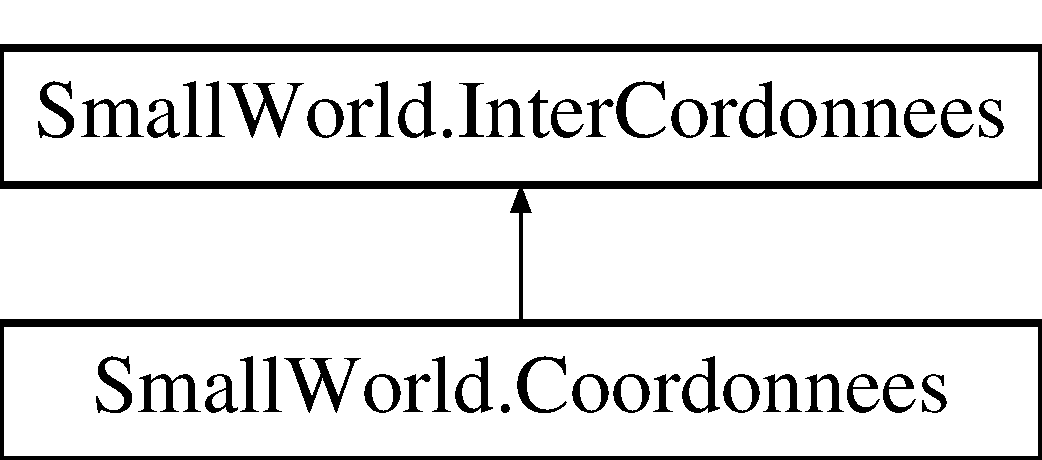
\includegraphics[height=2.000000cm]{class_small_world_1_1_coordonnees}
\end{center}
\end{figure}
\subsection*{Public Member Functions}
\begin{DoxyCompactItemize}
\item 
\hyperlink{class_small_world_1_1_coordonnees_aec13aa49810f6cb62c6b73c04fa9ebbe}{Coordonnees} (int abs, int ord)
\begin{DoxyCompactList}\small\item\em Constructeur de coordonnees. \end{DoxyCompactList}\item 
\hyperlink{class_small_world_1_1_coordonnees_a3e91ea13cf001b39eb63ca45345fd058}{Coordonnees} ()
\begin{DoxyCompactList}\small\item\em Constructeur de coordonnees. \end{DoxyCompactList}\item 
override bool \hyperlink{class_small_world_1_1_coordonnees_aa5bcb46ee14473b4a7c62442f7290ce1}{Equals} (Object obj)
\begin{DoxyCompactList}\small\item\em Test d'égalité pour deux coordonnées. \end{DoxyCompactList}\item 
override int \hyperlink{class_small_world_1_1_coordonnees_a8e05913286d547f5261480d8f03c5453}{Get\-Hash\-Code} ()
\begin{DoxyCompactList}\small\item\em return la clef de hash de l'objet \end{DoxyCompactList}\end{DoxyCompactItemize}
\subsection*{Properties}
\begin{DoxyCompactItemize}
\item 
\hypertarget{class_small_world_1_1_coordonnees_a08f32128a4ff9c97430d4ae8075c444a}{int \hyperlink{class_small_world_1_1_coordonnees_a08f32128a4ff9c97430d4ae8075c444a}{Abscisse}\hspace{0.3cm}{\ttfamily  \mbox{[}get, set\mbox{]}}}\label{class_small_world_1_1_coordonnees_a08f32128a4ff9c97430d4ae8075c444a}

\begin{DoxyCompactList}\small\item\em \hyperlink{namespace_small_world_1_1_properties}{Properties} pour l'attribut abscisse. \end{DoxyCompactList}\item 
\hypertarget{class_small_world_1_1_coordonnees_aac7114725ff9eaa08f7cc8588a13ed49}{int \hyperlink{class_small_world_1_1_coordonnees_aac7114725ff9eaa08f7cc8588a13ed49}{Ordonnee}\hspace{0.3cm}{\ttfamily  \mbox{[}get, set\mbox{]}}}\label{class_small_world_1_1_coordonnees_aac7114725ff9eaa08f7cc8588a13ed49}

\begin{DoxyCompactList}\small\item\em \hyperlink{namespace_small_world_1_1_properties}{Properties} pour l'attribut ordonnee. \end{DoxyCompactList}\end{DoxyCompactItemize}


\subsection{Detailed Description}
Rprésentation des coordonnées. 

\subsection{Constructor \& Destructor Documentation}
\hypertarget{class_small_world_1_1_coordonnees_aec13aa49810f6cb62c6b73c04fa9ebbe}{\index{Small\-World\-::\-Coordonnees@{Small\-World\-::\-Coordonnees}!Coordonnees@{Coordonnees}}
\index{Coordonnees@{Coordonnees}!SmallWorld::Coordonnees@{Small\-World\-::\-Coordonnees}}
\subsubsection[{Coordonnees}]{\setlength{\rightskip}{0pt plus 5cm}Small\-World.\-Coordonnees.\-Coordonnees (
\begin{DoxyParamCaption}
\item[{int}]{abs, }
\item[{int}]{ord}
\end{DoxyParamCaption}
)}}\label{class_small_world_1_1_coordonnees_aec13aa49810f6cb62c6b73c04fa9ebbe}


Constructeur de coordonnees. 


\begin{DoxyParams}{Parameters}
{\em int} & {\bfseries abs} L'abscisse \\
\hline
{\em int} & {\bfseries ord} L'ordonnée \\
\hline
\end{DoxyParams}
\begin{DoxyReturn}{Returns}
les nouvelles coordonnées 
\end{DoxyReturn}
\hypertarget{class_small_world_1_1_coordonnees_a3e91ea13cf001b39eb63ca45345fd058}{\index{Small\-World\-::\-Coordonnees@{Small\-World\-::\-Coordonnees}!Coordonnees@{Coordonnees}}
\index{Coordonnees@{Coordonnees}!SmallWorld::Coordonnees@{Small\-World\-::\-Coordonnees}}
\subsubsection[{Coordonnees}]{\setlength{\rightskip}{0pt plus 5cm}Small\-World.\-Coordonnees.\-Coordonnees (
\begin{DoxyParamCaption}
{}
\end{DoxyParamCaption}
)}}\label{class_small_world_1_1_coordonnees_a3e91ea13cf001b39eb63ca45345fd058}


Constructeur de coordonnees. 

\begin{DoxyReturn}{Returns}
les nouvelles coordonnées 
\end{DoxyReturn}


\subsection{Member Function Documentation}
\hypertarget{class_small_world_1_1_coordonnees_aa5bcb46ee14473b4a7c62442f7290ce1}{\index{Small\-World\-::\-Coordonnees@{Small\-World\-::\-Coordonnees}!Equals@{Equals}}
\index{Equals@{Equals}!SmallWorld::Coordonnees@{Small\-World\-::\-Coordonnees}}
\subsubsection[{Equals}]{\setlength{\rightskip}{0pt plus 5cm}Small\-World.\-Coordonnees.\-Equals (
\begin{DoxyParamCaption}
\item[{Object}]{obj}
\end{DoxyParamCaption}
)}}\label{class_small_world_1_1_coordonnees_aa5bcb46ee14473b4a7c62442f7290ce1}


Test d'égalité pour deux coordonnées. 


\begin{DoxyParams}{Parameters}
{\em Object} & {\bfseries obj} la coordonnée à comparer \\
\hline
\end{DoxyParams}
\begin{DoxyReturn}{Returns}
bool vrai si les deux coordonnées sont égales, faux sinon 
\end{DoxyReturn}
\hypertarget{class_small_world_1_1_coordonnees_a8e05913286d547f5261480d8f03c5453}{\index{Small\-World\-::\-Coordonnees@{Small\-World\-::\-Coordonnees}!Get\-Hash\-Code@{Get\-Hash\-Code}}
\index{Get\-Hash\-Code@{Get\-Hash\-Code}!SmallWorld::Coordonnees@{Small\-World\-::\-Coordonnees}}
\subsubsection[{Get\-Hash\-Code}]{\setlength{\rightskip}{0pt plus 5cm}Small\-World.\-Coordonnees.\-Get\-Hash\-Code (
\begin{DoxyParamCaption}
{}
\end{DoxyParamCaption}
)}}\label{class_small_world_1_1_coordonnees_a8e05913286d547f5261480d8f03c5453}


return la clef de hash de l'objet 

\begin{DoxyReturn}{Returns}
int la clef de hash 
\end{DoxyReturn}


The documentation for this class was generated from the following file\-:\begin{DoxyCompactItemize}
\item 
C\-:/\-Users/damienc/\-Documents/\-Git\-Hub/\-Small\-World/\-Visual\-Studio/\-Projet\-P\-O\-O/\hyperlink{_coordonnees_8cs}{Coordonnees.\-cs}\end{DoxyCompactItemize}

\hypertarget{class_small_world_1_1_createur_partie}{\section{Small\-World.\-Createur\-Partie Class Reference}
\label{class_small_world_1_1_createur_partie}\index{Small\-World.\-Createur\-Partie@{Small\-World.\-Createur\-Partie}}
}


Class du créateur de partie.  


Inheritance diagram for Small\-World.\-Createur\-Partie\-:\begin{figure}[H]
\begin{center}
\leavevmode
\includegraphics[height=2.000000cm]{class_small_world_1_1_createur_partie}
\end{center}
\end{figure}
\subsection*{Public Member Functions}
\begin{DoxyCompactItemize}
\item 
\hypertarget{class_small_world_1_1_createur_partie_a6c808936d929f91fa222ec40dde0105a}{void \hyperlink{class_small_world_1_1_createur_partie_a6c808936d929f91fa222ec40dde0105a}{construire} ()}\label{class_small_world_1_1_createur_partie_a6c808936d929f91fa222ec40dde0105a}

\begin{DoxyCompactList}\small\item\em Construction d'une nouvelle partie. \end{DoxyCompactList}\item 
\hypertarget{class_small_world_1_1_createur_partie_a9e8071dc3842e4389624728e84907008}{void {\bfseries ajouter\-Joueur} (string nom, string peuple)}\label{class_small_world_1_1_createur_partie_a9e8071dc3842e4389624728e84907008}

\item 
\hypertarget{class_small_world_1_1_createur_partie_ab8bc779d1ffd06f5715e43876e68aabf}{void {\bfseries ajouter\-Carte} ()}\label{class_small_world_1_1_createur_partie_ab8bc779d1ffd06f5715e43876e68aabf}

\end{DoxyCompactItemize}
\subsection*{Properties}
\begin{DoxyCompactItemize}
\item 
\hypertarget{class_small_world_1_1_createur_partie_a9e93618a0b35e91b328df64ba8816164}{\hyperlink{class_small_world_1_1_monteur_partie}{Monteur\-Partie} \hyperlink{class_small_world_1_1_createur_partie_a9e93618a0b35e91b328df64ba8816164}{Monteur\-Partie}\hspace{0.3cm}{\ttfamily  \mbox{[}get, set\mbox{]}}}\label{class_small_world_1_1_createur_partie_a9e93618a0b35e91b328df64ba8816164}

\begin{DoxyCompactList}\small\item\em Attribut permettant de monter une partie. \end{DoxyCompactList}\end{DoxyCompactItemize}


\subsection{Detailed Description}
Class du créateur de partie. 

The documentation for this class was generated from the following file\-:\begin{DoxyCompactItemize}
\item 
C\-:/\-Users/damienc/\-Documents/\-Git\-Hub/\-Small\-World/\-Visual\-Studio/\-Projet\-P\-O\-O/\hyperlink{_createur_partie_8cs}{Createur\-Partie.\-cs}\end{DoxyCompactItemize}

\hypertarget{class_small_world_1_1_desert}{\section{Small\-World.\-Desert Class Reference}
\label{class_small_world_1_1_desert}\index{Small\-World.\-Desert@{Small\-World.\-Desert}}
}
Inheritance diagram for Small\-World.\-Desert\-:\begin{figure}[H]
\begin{center}
\leavevmode
\includegraphics[height=3.000000cm]{class_small_world_1_1_desert}
\end{center}
\end{figure}
\subsection*{Additional Inherited Members}


The documentation for this class was generated from the following file\-:\begin{DoxyCompactItemize}
\item 
C\-:/\-Users/damienc/\-Documents/\-Git\-Hub/\-Small\-World/\-Visual\-Studio/\-Projet\-P\-O\-O/Case.\-cs\end{DoxyCompactItemize}

\hypertarget{class_small_world_1_1_eau}{\section{Small\-World.\-Eau Class Reference}
\label{class_small_world_1_1_eau}\index{Small\-World.\-Eau@{Small\-World.\-Eau}}
}
Inheritance diagram for Small\-World.\-Eau\-:\begin{figure}[H]
\begin{center}
\leavevmode
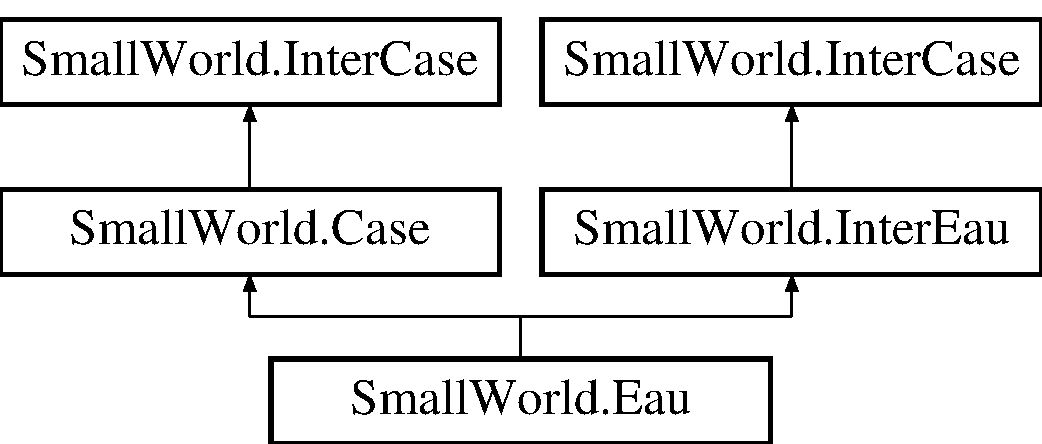
\includegraphics[height=3.000000cm]{class_small_world_1_1_eau}
\end{center}
\end{figure}
\subsection*{Additional Inherited Members}


The documentation for this class was generated from the following file\-:\begin{DoxyCompactItemize}
\item 
C\-:/\-Users/damienc/\-Documents/\-Git\-Hub/\-Small\-World/\-Visual\-Studio/\-Projet\-P\-O\-O/Case.\-cs\end{DoxyCompactItemize}

\hypertarget{interface_small_world_1_1_fabrique___unite___gaulois}{\section{Small\-World.\-Fabrique\-\_\-\-Unite\-\_\-\-Gaulois Interface Reference}
\label{interface_small_world_1_1_fabrique___unite___gaulois}\index{Small\-World.\-Fabrique\-\_\-\-Unite\-\_\-\-Gaulois@{Small\-World.\-Fabrique\-\_\-\-Unite\-\_\-\-Gaulois}}
}
Inheritance diagram for Small\-World.\-Fabrique\-\_\-\-Unite\-\_\-\-Gaulois\-:\begin{figure}[H]
\begin{center}
\leavevmode
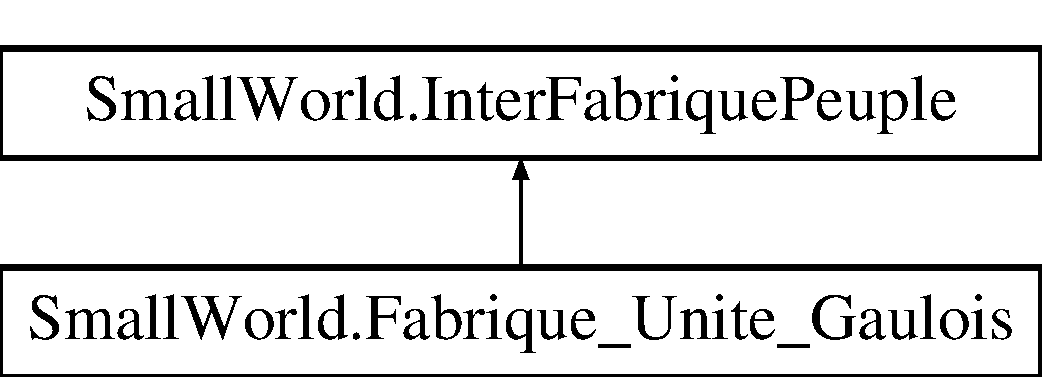
\includegraphics[height=2.000000cm]{interface_small_world_1_1_fabrique___unite___gaulois}
\end{center}
\end{figure}
\subsection*{Additional Inherited Members}


The documentation for this interface was generated from the following file\-:\begin{DoxyCompactItemize}
\item 
C\-:/\-Users/damienc/\-Documents/\-Git\-Hub/\-Small\-World/\-Visual\-Studio/\-Projet\-P\-O\-O/Fabrique\-Peuple.\-cs\end{DoxyCompactItemize}

\hypertarget{interface_small_world_1_1_fabrique___unite___nain}{\section{Small\-World.\-Fabrique\-\_\-\-Unite\-\_\-\-Nain Interface Reference}
\label{interface_small_world_1_1_fabrique___unite___nain}\index{Small\-World.\-Fabrique\-\_\-\-Unite\-\_\-\-Nain@{Small\-World.\-Fabrique\-\_\-\-Unite\-\_\-\-Nain}}
}
Inheritance diagram for Small\-World.\-Fabrique\-\_\-\-Unite\-\_\-\-Nain\-:\begin{figure}[H]
\begin{center}
\leavevmode
\includegraphics[height=2.000000cm]{interface_small_world_1_1_fabrique___unite___nain}
\end{center}
\end{figure}
\subsection*{Additional Inherited Members}


The documentation for this interface was generated from the following file\-:\begin{DoxyCompactItemize}
\item 
C\-:/\-Users/damienc/\-Documents/\-Git\-Hub/\-Small\-World/\-Visual\-Studio/\-Projet\-P\-O\-O/Fabrique\-Nain.\-cs\end{DoxyCompactItemize}

\hypertarget{interface_small_world_1_1_fabrique___unite___viking}{\section{Small\-World.\-Fabrique\-\_\-\-Unite\-\_\-\-Viking Interface Reference}
\label{interface_small_world_1_1_fabrique___unite___viking}\index{Small\-World.\-Fabrique\-\_\-\-Unite\-\_\-\-Viking@{Small\-World.\-Fabrique\-\_\-\-Unite\-\_\-\-Viking}}
}
Inheritance diagram for Small\-World.\-Fabrique\-\_\-\-Unite\-\_\-\-Viking\-:\begin{figure}[H]
\begin{center}
\leavevmode
\includegraphics[height=2.000000cm]{interface_small_world_1_1_fabrique___unite___viking}
\end{center}
\end{figure}
\subsection*{Additional Inherited Members}


The documentation for this interface was generated from the following file\-:\begin{DoxyCompactItemize}
\item 
C\-:/\-Users/damienc/\-Documents/\-Git\-Hub/\-Small\-World/\-Visual\-Studio/\-Projet\-P\-O\-O/Fabrique\-Viking.\-cs\end{DoxyCompactItemize}

\hypertarget{class_small_world_1_1_fabrique_case}{\section{Small\-World.\-Fabrique\-Case Class Reference}
\label{class_small_world_1_1_fabrique_case}\index{Small\-World.\-Fabrique\-Case@{Small\-World.\-Fabrique\-Case}}
}
Inheritance diagram for Small\-World.\-Fabrique\-Case\-:\begin{figure}[H]
\begin{center}
\leavevmode
\includegraphics[height=2.000000cm]{class_small_world_1_1_fabrique_case}
\end{center}
\end{figure}
\subsection*{Public Member Functions}
\begin{DoxyCompactItemize}
\item 
\hypertarget{class_small_world_1_1_fabrique_case_aa79573e726becd0bca9e014646c4f78b}{void {\bfseries obtenir\-Eau} ()}\label{class_small_world_1_1_fabrique_case_aa79573e726becd0bca9e014646c4f78b}

\item 
\hypertarget{class_small_world_1_1_fabrique_case_acc6cf14d1993e782a1ed89a7e1a27ea5}{void {\bfseries obtenir\-Montagne} ()}\label{class_small_world_1_1_fabrique_case_acc6cf14d1993e782a1ed89a7e1a27ea5}

\item 
\hypertarget{class_small_world_1_1_fabrique_case_a4f9585f6b5f56bdbed9ea60822456975}{void {\bfseries obtenir\-Desert} ()}\label{class_small_world_1_1_fabrique_case_a4f9585f6b5f56bdbed9ea60822456975}

\item 
\hypertarget{class_small_world_1_1_fabrique_case_a45ddb3587cb1eea8cedab4c7b6eb0c36}{void {\bfseries obtenir\-Plaine} ()}\label{class_small_world_1_1_fabrique_case_a45ddb3587cb1eea8cedab4c7b6eb0c36}

\item 
\hypertarget{class_small_world_1_1_fabrique_case_a8ab32b492139c98b86c4d9cd011cc70a}{void {\bfseries obtenir\-Foret} ()}\label{class_small_world_1_1_fabrique_case_a8ab32b492139c98b86c4d9cd011cc70a}

\item 
\hypertarget{class_small_world_1_1_fabrique_case_a4e8866effdb5680f02dc43b49e599d0c}{void {\bfseries obtenir\-Case} ()}\label{class_small_world_1_1_fabrique_case_a4e8866effdb5680f02dc43b49e599d0c}

\end{DoxyCompactItemize}
\subsection*{Properties}
\begin{DoxyCompactItemize}
\item 
\hypertarget{class_small_world_1_1_fabrique_case_a800e3f658e67dcd6ab269386ed08dc2f}{\hyperlink{class_small_world_1_1_foret}{Foret} {\bfseries Foret}\hspace{0.3cm}{\ttfamily  \mbox{[}get, set\mbox{]}}}\label{class_small_world_1_1_fabrique_case_a800e3f658e67dcd6ab269386ed08dc2f}

\item 
\hypertarget{class_small_world_1_1_fabrique_case_a97131f6c0a1bc3ceeedf98059fbba0c1}{\hyperlink{class_small_world_1_1_plaine}{Plaine} {\bfseries Plaine}\hspace{0.3cm}{\ttfamily  \mbox{[}get, set\mbox{]}}}\label{class_small_world_1_1_fabrique_case_a97131f6c0a1bc3ceeedf98059fbba0c1}

\item 
\hypertarget{class_small_world_1_1_fabrique_case_a960d80498fb7512f1bc57e30b900b958}{\hyperlink{class_small_world_1_1_desert}{Desert} {\bfseries Desert}\hspace{0.3cm}{\ttfamily  \mbox{[}get, set\mbox{]}}}\label{class_small_world_1_1_fabrique_case_a960d80498fb7512f1bc57e30b900b958}

\item 
\hypertarget{class_small_world_1_1_fabrique_case_a6b633850fecde0d1a9a42b65eb73b248}{\hyperlink{class_small_world_1_1_montagne}{Montagne} {\bfseries Montagne}\hspace{0.3cm}{\ttfamily  \mbox{[}get, set\mbox{]}}}\label{class_small_world_1_1_fabrique_case_a6b633850fecde0d1a9a42b65eb73b248}

\item 
\hypertarget{class_small_world_1_1_fabrique_case_aa247bfdc40a15c5738d48d55e56ad169}{\hyperlink{class_small_world_1_1_eau}{Eau} {\bfseries Eau}\hspace{0.3cm}{\ttfamily  \mbox{[}get, set\mbox{]}}}\label{class_small_world_1_1_fabrique_case_aa247bfdc40a15c5738d48d55e56ad169}

\end{DoxyCompactItemize}


The documentation for this class was generated from the following file\-:\begin{DoxyCompactItemize}
\item 
C\-:/\-Users/damienc/\-Documents/\-Git\-Hub/\-Small\-World/\-Visual\-Studio/\-Projet\-P\-O\-O/Fabrique\-Case.\-cs\end{DoxyCompactItemize}

\hypertarget{interface_small_world_1_1_fabrique_jeu}{\section{Small\-World.\-Fabrique\-Jeu Interface Reference}
\label{interface_small_world_1_1_fabrique_jeu}\index{Small\-World.\-Fabrique\-Jeu@{Small\-World.\-Fabrique\-Jeu}}
}
\subsection*{Public Member Functions}
\begin{DoxyCompactItemize}
\item 
\hypertarget{interface_small_world_1_1_fabrique_jeu_a47c9d5ecca334a92c89a2e6ec8d862af}{void {\bfseries creer\-Partie} ()}\label{interface_small_world_1_1_fabrique_jeu_a47c9d5ecca334a92c89a2e6ec8d862af}

\item 
\hypertarget{interface_small_world_1_1_fabrique_jeu_a5fbfc360cc9d656f23725c33f6b0d383}{void {\bfseries creer\-Joueur} (string nom\-Joueur, string \hyperlink{class_small_world_1_1_peuple}{Peuple})}\label{interface_small_world_1_1_fabrique_jeu_a5fbfc360cc9d656f23725c33f6b0d383}

\item 
\hypertarget{interface_small_world_1_1_fabrique_jeu_a4d323908250275fa5b62eed7cad3f4ab}{void {\bfseries charger\-Partie} ()}\label{interface_small_world_1_1_fabrique_jeu_a4d323908250275fa5b62eed7cad3f4ab}

\end{DoxyCompactItemize}


The documentation for this interface was generated from the following file\-:\begin{DoxyCompactItemize}
\item 
C\-:/\-Users/damienc/\-Documents/\-Git\-Hub/\-Small\-World/\-Visual\-Studio/\-Projet\-P\-O\-O/Fabrique\-Jeu.\-cs\end{DoxyCompactItemize}

\hypertarget{class_small_world_1_1_fabrique_peuple}{\section{Small\-World.\-Fabrique\-Peuple Class Reference}
\label{class_small_world_1_1_fabrique_peuple}\index{Small\-World.\-Fabrique\-Peuple@{Small\-World.\-Fabrique\-Peuple}}
}


classe pour la fabrique d'un peuple  


Inheritance diagram for Small\-World.\-Fabrique\-Peuple\-:\begin{figure}[H]
\begin{center}
\leavevmode
\includegraphics[height=2.000000cm]{class_small_world_1_1_fabrique_peuple}
\end{center}
\end{figure}
\subsection*{Public Member Functions}
\begin{DoxyCompactItemize}
\item 
\hypertarget{class_small_world_1_1_fabrique_peuple_a5fe5672eb02c7fb6f0aedccfe490b3b9}{\hyperlink{class_small_world_1_1_fabrique_peuple_a5fe5672eb02c7fb6f0aedccfe490b3b9}{Fabrique\-Peuple} ()}\label{class_small_world_1_1_fabrique_peuple_a5fe5672eb02c7fb6f0aedccfe490b3b9}

\begin{DoxyCompactList}\small\item\em Constructeur d'une fabrique de peuple. \end{DoxyCompactList}\item 
\hyperlink{class_small_world_1_1_peuple}{Peuple} \hyperlink{class_small_world_1_1_fabrique_peuple_ad3c21feceaebffdbfc0bdcb66edc4bdb}{fabriquer\-Peuple} (string peuple)
\begin{DoxyCompactList}\small\item\em Récupération d'un peuple. \end{DoxyCompactList}\end{DoxyCompactItemize}
\subsection*{Properties}
\begin{DoxyCompactItemize}
\item 
\hypertarget{class_small_world_1_1_fabrique_peuple_a2d46d0022cccca8e6fa8a44c097aea6a}{static \hyperlink{class_small_world_1_1_fabrique_peuple}{Fabrique\-Peuple} \hyperlink{class_small_world_1_1_fabrique_peuple_a2d46d0022cccca8e6fa8a44c097aea6a}{Instance\-\_\-\-Fab\-Peuple}\hspace{0.3cm}{\ttfamily  \mbox{[}get\mbox{]}}}\label{class_small_world_1_1_fabrique_peuple_a2d46d0022cccca8e6fa8a44c097aea6a}

\begin{DoxyCompactList}\small\item\em \hyperlink{namespace_small_world_1_1_properties}{Properties} pour l'attribut instance\-\_\-\-Fab\-Peuple. \end{DoxyCompactList}\end{DoxyCompactItemize}


\subsection{Detailed Description}
classe pour la fabrique d'un peuple 

\hyperlink{class_small_world_1_1_fabrique_peuple}{Fabrique\-Peuple} est un singleton 

\subsection{Member Function Documentation}
\hypertarget{class_small_world_1_1_fabrique_peuple_ad3c21feceaebffdbfc0bdcb66edc4bdb}{\index{Small\-World\-::\-Fabrique\-Peuple@{Small\-World\-::\-Fabrique\-Peuple}!fabriquer\-Peuple@{fabriquer\-Peuple}}
\index{fabriquer\-Peuple@{fabriquer\-Peuple}!SmallWorld::FabriquePeuple@{Small\-World\-::\-Fabrique\-Peuple}}
\subsubsection[{fabriquer\-Peuple}]{\setlength{\rightskip}{0pt plus 5cm}Small\-World.\-Fabrique\-Peuple.\-fabriquer\-Peuple (
\begin{DoxyParamCaption}
\item[{string}]{peuple}
\end{DoxyParamCaption}
)}}\label{class_small_world_1_1_fabrique_peuple_ad3c21feceaebffdbfc0bdcb66edc4bdb}


Récupération d'un peuple. 


\begin{DoxyParams}{Parameters}
{\em string} & {\bfseries peuple} le peuple demandé \\
\hline
\end{DoxyParams}
\begin{DoxyReturn}{Returns}
\hyperlink{class_small_world_1_1_peuple}{Peuple} Le peuple 
\end{DoxyReturn}


Implements \hyperlink{interface_small_world_1_1_inter_fabrique_peuple_a5f4c738231b141ffc6afd295d259a80a}{Small\-World.\-Inter\-Fabrique\-Peuple}.



The documentation for this class was generated from the following file\-:\begin{DoxyCompactItemize}
\item 
C\-:/\-Users/damienc/\-Documents/\-Git\-Hub/\-Small\-World/\-Visual\-Studio/\-Projet\-P\-O\-O/\hyperlink{_fabrique_peuple_8cs}{Fabrique\-Peuple.\-cs}\end{DoxyCompactItemize}

\hypertarget{class_small_world_1_1_foret}{\section{Small\-World.\-Foret Class Reference}
\label{class_small_world_1_1_foret}\index{Small\-World.\-Foret@{Small\-World.\-Foret}}
}
Inheritance diagram for Small\-World.\-Foret\-:\begin{figure}[H]
\begin{center}
\leavevmode
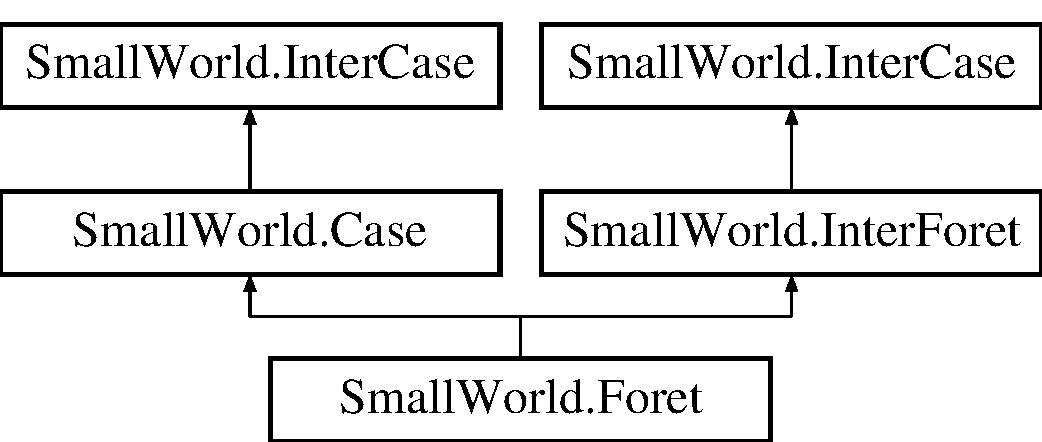
\includegraphics[height=3.000000cm]{class_small_world_1_1_foret}
\end{center}
\end{figure}
\subsection*{Additional Inherited Members}


The documentation for this class was generated from the following file\-:\begin{DoxyCompactItemize}
\item 
C\-:/\-Users/damienc/\-Documents/\-Git\-Hub/\-Small\-World/\-Visual\-Studio/\-Projet\-P\-O\-O/Case.\-cs\end{DoxyCompactItemize}

\hypertarget{interface_small_world_1_1_inter_carte}{\section{Small\-World.\-Inter\-Carte Interface Reference}
\label{interface_small_world_1_1_inter_carte}\index{Small\-World.\-Inter\-Carte@{Small\-World.\-Inter\-Carte}}
}


Interface pour \hyperlink{class_small_world_1_1_carte}{Carte}.  


Inheritance diagram for Small\-World.\-Inter\-Carte\-:\begin{figure}[H]
\begin{center}
\leavevmode
\includegraphics[height=2.000000cm]{interface_small_world_1_1_inter_carte}
\end{center}
\end{figure}
\subsection*{Public Member Functions}
\begin{DoxyCompactItemize}
\item 
void \hyperlink{interface_small_world_1_1_inter_carte_a825e1748eb1a8f93dfe8aecdfc661064}{creer\-Carte} ()
\begin{DoxyCompactList}\small\item\em Génération d'une nouvelle \hyperlink{class_small_world_1_1_carte}{Carte}. \end{DoxyCompactList}\item 
void \hyperlink{interface_small_world_1_1_inter_carte_a23c669cb523f222f53e8ab91a8944472}{definir\-Strategie} (\hyperlink{class_small_world_1_1_strategie_carte}{Strategie\-Carte} strat)
\begin{DoxyCompactList}\small\item\em Définit la stratégie à adopter pour la génération d'une nouvelle carte. \end{DoxyCompactList}\end{DoxyCompactItemize}


\subsection{Detailed Description}
Interface pour \hyperlink{class_small_world_1_1_carte}{Carte}. 

\subsection{Member Function Documentation}
\hypertarget{interface_small_world_1_1_inter_carte_a825e1748eb1a8f93dfe8aecdfc661064}{\index{Small\-World\-::\-Inter\-Carte@{Small\-World\-::\-Inter\-Carte}!creer\-Carte@{creer\-Carte}}
\index{creer\-Carte@{creer\-Carte}!SmallWorld::InterCarte@{Small\-World\-::\-Inter\-Carte}}
\subsubsection[{creer\-Carte}]{\setlength{\rightskip}{0pt plus 5cm}Small\-World.\-Inter\-Carte.\-creer\-Carte (
\begin{DoxyParamCaption}
{}
\end{DoxyParamCaption}
)}}\label{interface_small_world_1_1_inter_carte_a825e1748eb1a8f93dfe8aecdfc661064}


Génération d'une nouvelle \hyperlink{class_small_world_1_1_carte}{Carte}. 

Génère une nouvelle \hyperlink{class_small_world_1_1_carte}{Carte}, suivant la stratégie demandée

\begin{DoxyReturn}{Returns}
void 
\end{DoxyReturn}


Implemented in \hyperlink{class_small_world_1_1_carte_a412690bcb32264b5282913660c5e38f8}{Small\-World.\-Carte}.

\hypertarget{interface_small_world_1_1_inter_carte_a23c669cb523f222f53e8ab91a8944472}{\index{Small\-World\-::\-Inter\-Carte@{Small\-World\-::\-Inter\-Carte}!definir\-Strategie@{definir\-Strategie}}
\index{definir\-Strategie@{definir\-Strategie}!SmallWorld::InterCarte@{Small\-World\-::\-Inter\-Carte}}
\subsubsection[{definir\-Strategie}]{\setlength{\rightskip}{0pt plus 5cm}Small\-World.\-Inter\-Carte.\-definir\-Strategie (
\begin{DoxyParamCaption}
\item[{{\bf Strategie\-Carte}}]{strat}
\end{DoxyParamCaption}
)}}\label{interface_small_world_1_1_inter_carte_a23c669cb523f222f53e8ab91a8944472}


Définit la stratégie à adopter pour la génération d'une nouvelle carte. 


\begin{DoxyParams}{Parameters}
{\em \hyperlink{class_small_world_1_1_strategie_carte}{Strategie\-Carte}} & {\bfseries strat} La nouvelle stratégie à adopter \\
\hline
\end{DoxyParams}
\begin{DoxyReturn}{Returns}
void 
\end{DoxyReturn}


Implemented in \hyperlink{class_small_world_1_1_carte_aad692a68904925a11d5307181ca83c5f}{Small\-World.\-Carte}.



The documentation for this interface was generated from the following file\-:\begin{DoxyCompactItemize}
\item 
C\-:/\-Users/damienc/\-Documents/\-Git\-Hub/\-Small\-World/\-Visual\-Studio/\-Projet\-P\-O\-O/\hyperlink{_carte_8cs}{Carte.\-cs}\end{DoxyCompactItemize}

\hypertarget{interface_small_world_1_1_inter_case}{\section{Small\-World.\-Inter\-Case Interface Reference}
\label{interface_small_world_1_1_inter_case}\index{Small\-World.\-Inter\-Case@{Small\-World.\-Inter\-Case}}
}
Inheritance diagram for Small\-World.\-Inter\-Case\-:\begin{figure}[H]
\begin{center}
\leavevmode
\includegraphics[height=3.333333cm]{interface_small_world_1_1_inter_case}
\end{center}
\end{figure}


The documentation for this interface was generated from the following file\-:\begin{DoxyCompactItemize}
\item 
C\-:/\-Users/damienc/\-Documents/\-Git\-Hub/\-Small\-World/\-Visual\-Studio/\-Projet\-P\-O\-O/Case.\-cs\end{DoxyCompactItemize}

\hypertarget{interface_small_world_1_1_inter_createur_partie}{\section{Small\-World.\-Inter\-Createur\-Partie Interface Reference}
\label{interface_small_world_1_1_inter_createur_partie}\index{Small\-World.\-Inter\-Createur\-Partie@{Small\-World.\-Inter\-Createur\-Partie}}
}


Interface du créateur de partie.  


Inheritance diagram for Small\-World.\-Inter\-Createur\-Partie\-:\begin{figure}[H]
\begin{center}
\leavevmode
\includegraphics[height=2.000000cm]{interface_small_world_1_1_inter_createur_partie}
\end{center}
\end{figure}
\subsection*{Public Member Functions}
\begin{DoxyCompactItemize}
\item 
\hypertarget{interface_small_world_1_1_inter_createur_partie_a84bc048d2a71699fef54ef531477c917}{\hyperlink{class_small_world_1_1_partie}{Partie} \hyperlink{interface_small_world_1_1_inter_createur_partie_a84bc048d2a71699fef54ef531477c917}{construire} ()}\label{interface_small_world_1_1_inter_createur_partie_a84bc048d2a71699fef54ef531477c917}

\begin{DoxyCompactList}\small\item\em Construire la partie. \end{DoxyCompactList}\item 
void \hyperlink{interface_small_world_1_1_inter_createur_partie_af3fa5aaff01c6709b99eff93b6252da5}{ajout\-Joueur} (string nom, string peuple)
\begin{DoxyCompactList}\small\item\em Ajouter un joueur à la partie. \end{DoxyCompactList}\end{DoxyCompactItemize}


\subsection{Detailed Description}
Interface du créateur de partie. 

\subsection{Member Function Documentation}
\hypertarget{interface_small_world_1_1_inter_createur_partie_af3fa5aaff01c6709b99eff93b6252da5}{\index{Small\-World\-::\-Inter\-Createur\-Partie@{Small\-World\-::\-Inter\-Createur\-Partie}!ajout\-Joueur@{ajout\-Joueur}}
\index{ajout\-Joueur@{ajout\-Joueur}!SmallWorld::InterCreateurPartie@{Small\-World\-::\-Inter\-Createur\-Partie}}
\subsubsection[{ajout\-Joueur}]{\setlength{\rightskip}{0pt plus 5cm}Small\-World.\-Inter\-Createur\-Partie.\-ajout\-Joueur (
\begin{DoxyParamCaption}
\item[{string}]{nom, }
\item[{string}]{peuple}
\end{DoxyParamCaption}
)}}\label{interface_small_world_1_1_inter_createur_partie_af3fa5aaff01c6709b99eff93b6252da5}


Ajouter un joueur à la partie. 


\begin{DoxyParams}{Parameters}
{\em string} & {\bfseries nom} le nom du joueur \\
\hline
{\em string} & {\bfseries peuple} le type de peuple \\
\hline
\end{DoxyParams}
\begin{DoxyReturn}{Returns}
void 
\end{DoxyReturn}


Implemented in \hyperlink{class_small_world_1_1_createur_partie_a1388144440304d2d82879a15e0e58e1f}{Small\-World.\-Createur\-Partie}.



The documentation for this interface was generated from the following file\-:\begin{DoxyCompactItemize}
\item 
C\-:/\-Users/damienc/\-Documents/\-Git\-Hub/\-Small\-World/\-Visual\-Studio/\-Projet\-P\-O\-O/\hyperlink{_createur_partie_8cs}{Createur\-Partie.\-cs}\end{DoxyCompactItemize}

\hypertarget{interface_small_world_1_1_inter_desert}{\section{Small\-World.\-Inter\-Desert Interface Reference}
\label{interface_small_world_1_1_inter_desert}\index{Small\-World.\-Inter\-Desert@{Small\-World.\-Inter\-Desert}}
}
Inheritance diagram for Small\-World.\-Inter\-Desert\-:\begin{figure}[H]
\begin{center}
\leavevmode
\includegraphics[height=3.000000cm]{interface_small_world_1_1_inter_desert}
\end{center}
\end{figure}


The documentation for this interface was generated from the following file\-:\begin{DoxyCompactItemize}
\item 
C\-:/\-Users/damienc/\-Documents/\-Git\-Hub/\-Small\-World/\-Visual\-Studio/\-Projet\-P\-O\-O/Case.\-cs\end{DoxyCompactItemize}

\hypertarget{interface_small_world_1_1_inter_eau}{\section{Small\-World.\-Inter\-Eau Interface Reference}
\label{interface_small_world_1_1_inter_eau}\index{Small\-World.\-Inter\-Eau@{Small\-World.\-Inter\-Eau}}
}
Inheritance diagram for Small\-World.\-Inter\-Eau\-:\begin{figure}[H]
\begin{center}
\leavevmode
\includegraphics[height=3.000000cm]{interface_small_world_1_1_inter_eau}
\end{center}
\end{figure}


The documentation for this interface was generated from the following file\-:\begin{DoxyCompactItemize}
\item 
C\-:/\-Users/damienc/\-Documents/\-Git\-Hub/\-Small\-World/\-Visual\-Studio/\-Projet\-P\-O\-O/Case.\-cs\end{DoxyCompactItemize}

\hypertarget{interface_small_world_1_1_inter_fabrique_case}{\section{Small\-World.\-Inter\-Fabrique\-Case Interface Reference}
\label{interface_small_world_1_1_inter_fabrique_case}\index{Small\-World.\-Inter\-Fabrique\-Case@{Small\-World.\-Inter\-Fabrique\-Case}}
}
Inheritance diagram for Small\-World.\-Inter\-Fabrique\-Case\-:\begin{figure}[H]
\begin{center}
\leavevmode
\includegraphics[height=2.000000cm]{interface_small_world_1_1_inter_fabrique_case}
\end{center}
\end{figure}
\subsection*{Public Member Functions}
\begin{DoxyCompactItemize}
\item 
\hypertarget{interface_small_world_1_1_inter_fabrique_case_a1434bcec9bf29cfd87d80bb0b71c709c}{\hyperlink{class_small_world_1_1_case}{Case} {\bfseries obtenir\-Eau} ()}\label{interface_small_world_1_1_inter_fabrique_case_a1434bcec9bf29cfd87d80bb0b71c709c}

\item 
\hypertarget{interface_small_world_1_1_inter_fabrique_case_af726293fdccaa7f5af1729551a6dd1ed}{\hyperlink{class_small_world_1_1_case}{Case} {\bfseries obtenir\-Montagne} ()}\label{interface_small_world_1_1_inter_fabrique_case_af726293fdccaa7f5af1729551a6dd1ed}

\item 
\hypertarget{interface_small_world_1_1_inter_fabrique_case_a9ffa841ddec5636b3241db2e4cf51b49}{\hyperlink{class_small_world_1_1_case}{Case} {\bfseries obtenir\-Desert} ()}\label{interface_small_world_1_1_inter_fabrique_case_a9ffa841ddec5636b3241db2e4cf51b49}

\item 
\hypertarget{interface_small_world_1_1_inter_fabrique_case_a8f35df965c3546307d905b2909dca774}{\hyperlink{class_small_world_1_1_case}{Case} {\bfseries obtenir\-Plaine} ()}\label{interface_small_world_1_1_inter_fabrique_case_a8f35df965c3546307d905b2909dca774}

\item 
\hypertarget{interface_small_world_1_1_inter_fabrique_case_aaf69be0da8fc845f9e8418e028cf41fc}{\hyperlink{class_small_world_1_1_case}{Case} {\bfseries obtenir\-Foret} ()}\label{interface_small_world_1_1_inter_fabrique_case_aaf69be0da8fc845f9e8418e028cf41fc}

\item 
\hypertarget{interface_small_world_1_1_inter_fabrique_case_a67a341c2ee1caef98513b5fe701e953b}{\hyperlink{class_small_world_1_1_case}{Case} {\bfseries obtenir\-Case} (int type\-Case)}\label{interface_small_world_1_1_inter_fabrique_case_a67a341c2ee1caef98513b5fe701e953b}

\end{DoxyCompactItemize}


The documentation for this interface was generated from the following file\-:\begin{DoxyCompactItemize}
\item 
C\-:/\-Users/damienc/\-Documents/\-Git\-Hub/\-Small\-World/\-Visual\-Studio/\-Projet\-P\-O\-O/Fabrique\-Case.\-cs\end{DoxyCompactItemize}

\hypertarget{interface_small_world_1_1_inter_fabrique_peuple}{\section{Small\-World.\-Inter\-Fabrique\-Peuple Interface Reference}
\label{interface_small_world_1_1_inter_fabrique_peuple}\index{Small\-World.\-Inter\-Fabrique\-Peuple@{Small\-World.\-Inter\-Fabrique\-Peuple}}
}
Inheritance diagram for Small\-World.\-Inter\-Fabrique\-Peuple\-:\begin{figure}[H]
\begin{center}
\leavevmode
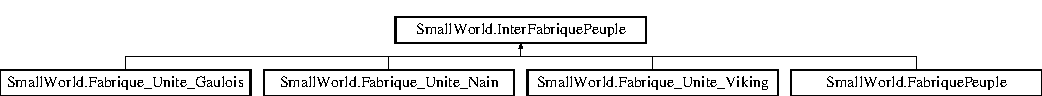
\includegraphics[height=1.266968cm]{interface_small_world_1_1_inter_fabrique_peuple}
\end{center}
\end{figure}
\subsection*{Public Member Functions}
\begin{DoxyCompactItemize}
\item 
\hypertarget{interface_small_world_1_1_inter_fabrique_peuple_a43c849b7b035e7ebf2e96128c75cd0ee}{void {\bfseries fabriquer\-Peuple} ()}\label{interface_small_world_1_1_inter_fabrique_peuple_a43c849b7b035e7ebf2e96128c75cd0ee}

\end{DoxyCompactItemize}


The documentation for this interface was generated from the following file\-:\begin{DoxyCompactItemize}
\item 
C\-:/\-Users/damienc/\-Documents/\-Git\-Hub/\-Small\-World/\-Visual\-Studio/\-Projet\-P\-O\-O/Fabrique.\-cs\end{DoxyCompactItemize}

\hypertarget{interface_small_world_1_1_inter_foret}{\section{Small\-World.\-Inter\-Foret Interface Reference}
\label{interface_small_world_1_1_inter_foret}\index{Small\-World.\-Inter\-Foret@{Small\-World.\-Inter\-Foret}}
}
Inheritance diagram for Small\-World.\-Inter\-Foret\-:\begin{figure}[H]
\begin{center}
\leavevmode
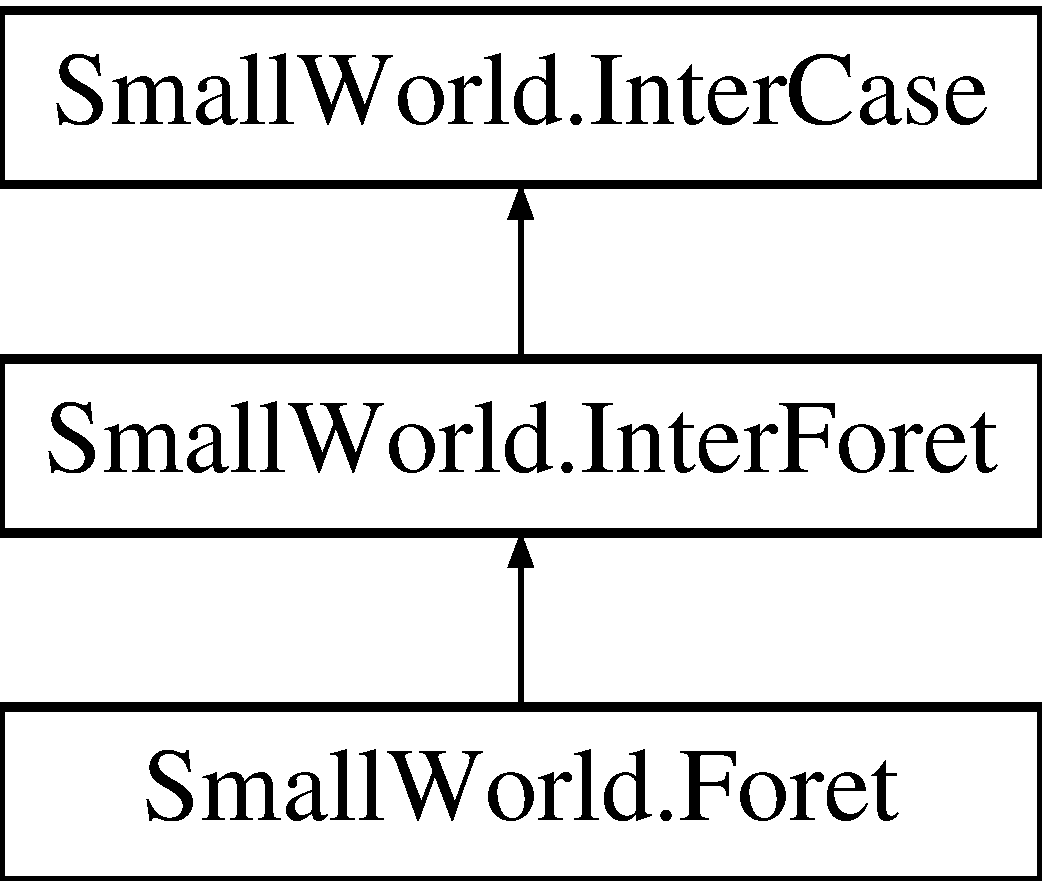
\includegraphics[height=3.000000cm]{interface_small_world_1_1_inter_foret}
\end{center}
\end{figure}


The documentation for this interface was generated from the following file\-:\begin{DoxyCompactItemize}
\item 
C\-:/\-Users/damienc/\-Documents/\-Git\-Hub/\-Small\-World/\-Visual\-Studio/\-Projet\-P\-O\-O/foret.\-cs\end{DoxyCompactItemize}

\hypertarget{interface_small_world_1_1_inter_joueur}{\section{Small\-World.\-Inter\-Joueur Interface Reference}
\label{interface_small_world_1_1_inter_joueur}\index{Small\-World.\-Inter\-Joueur@{Small\-World.\-Inter\-Joueur}}
}
Inheritance diagram for Small\-World.\-Inter\-Joueur\-:\begin{figure}[H]
\begin{center}
\leavevmode
\includegraphics[height=2.000000cm]{interface_small_world_1_1_inter_joueur}
\end{center}
\end{figure}


The documentation for this interface was generated from the following file\-:\begin{DoxyCompactItemize}
\item 
C\-:/\-Users/damienc/\-Documents/\-Git\-Hub/\-Small\-World/\-Visual\-Studio/\-Projet\-P\-O\-O/Joueur.\-cs\end{DoxyCompactItemize}

\hypertarget{interface_small_world_1_1_inter_montagne}{\section{Small\-World.\-Inter\-Montagne Interface Reference}
\label{interface_small_world_1_1_inter_montagne}\index{Small\-World.\-Inter\-Montagne@{Small\-World.\-Inter\-Montagne}}
}
Inheritance diagram for Small\-World.\-Inter\-Montagne\-:\begin{figure}[H]
\begin{center}
\leavevmode
\includegraphics[height=3.000000cm]{interface_small_world_1_1_inter_montagne}
\end{center}
\end{figure}


The documentation for this interface was generated from the following file\-:\begin{DoxyCompactItemize}
\item 
C\-:/\-Users/damienc/\-Documents/\-Git\-Hub/\-Small\-World/\-Visual\-Studio/\-Projet\-P\-O\-O/montagne.\-cs\end{DoxyCompactItemize}

\hypertarget{interface_small_world_1_1_inter_monteur_partie}{\section{Small\-World.\-Inter\-Monteur\-Partie Interface Reference}
\label{interface_small_world_1_1_inter_monteur_partie}\index{Small\-World.\-Inter\-Monteur\-Partie@{Small\-World.\-Inter\-Monteur\-Partie}}
}


Interface globale du monteur.  


Inheritance diagram for Small\-World.\-Inter\-Monteur\-Partie\-:\begin{figure}[H]
\begin{center}
\leavevmode
\includegraphics[height=1.171548cm]{interface_small_world_1_1_inter_monteur_partie}
\end{center}
\end{figure}
\subsection*{Public Member Functions}
\begin{DoxyCompactItemize}
\item 
void \hyperlink{interface_small_world_1_1_inter_monteur_partie_a473c91ad26ee485f07261df1fcae0e8b}{ajouter\-Carte} ()
\begin{DoxyCompactList}\small\item\em Ajout de la carte pour la construction d'une partie. \end{DoxyCompactList}\item 
void \hyperlink{interface_small_world_1_1_inter_monteur_partie_ae52498262dd36230b0c0d090cb59ff07}{ajouter\-Joueur} (string nom\-Joueur, string peuple)
\begin{DoxyCompactList}\small\item\em Ajout d'un joueur à la partie. \end{DoxyCompactList}\item 
\hyperlink{class_small_world_1_1_partie}{Partie} \hyperlink{interface_small_world_1_1_inter_monteur_partie_ad471ab6610aaa1664fb3d0bd93f00be3}{creer\-Partie} (string nom\-Joueur\-A, string peuple\-A, string nom\-Joueur\-B, string peuple\-B)
\begin{DoxyCompactList}\small\item\em Création de la partie. \end{DoxyCompactList}\item 
void \hyperlink{interface_small_world_1_1_inter_monteur_partie_a4ea7442b592d23a0f31e0d0020f124de}{placer\-Unites} ()
\begin{DoxyCompactList}\small\item\em Placement des unités avant le début de la partie. \end{DoxyCompactList}\item 
void \hyperlink{interface_small_world_1_1_inter_monteur_partie_afa1b718338a15b4dd0deb5d817f3484c}{initialiser\-Nombre\-Tour} ()
\begin{DoxyCompactList}\small\item\em initialise le nombre de tour d'un partie \end{DoxyCompactList}\end{DoxyCompactItemize}


\subsection{Detailed Description}
Interface globale du monteur. 

\subsection{Member Function Documentation}
\hypertarget{interface_small_world_1_1_inter_monteur_partie_a473c91ad26ee485f07261df1fcae0e8b}{\index{Small\-World\-::\-Inter\-Monteur\-Partie@{Small\-World\-::\-Inter\-Monteur\-Partie}!ajouter\-Carte@{ajouter\-Carte}}
\index{ajouter\-Carte@{ajouter\-Carte}!SmallWorld::InterMonteurPartie@{Small\-World\-::\-Inter\-Monteur\-Partie}}
\subsubsection[{ajouter\-Carte}]{\setlength{\rightskip}{0pt plus 5cm}Small\-World.\-Inter\-Monteur\-Partie.\-ajouter\-Carte (
\begin{DoxyParamCaption}
{}
\end{DoxyParamCaption}
)}}\label{interface_small_world_1_1_inter_monteur_partie_a473c91ad26ee485f07261df1fcae0e8b}


Ajout de la carte pour la construction d'une partie. 

\begin{DoxyReturn}{Returns}
void 
\end{DoxyReturn}


Implemented in \hyperlink{class_small_world_1_1_monteur_partie_ad8cedb326193c0f0ff5f2d6705867156}{Small\-World.\-Monteur\-Partie}.

\hypertarget{interface_small_world_1_1_inter_monteur_partie_ae52498262dd36230b0c0d090cb59ff07}{\index{Small\-World\-::\-Inter\-Monteur\-Partie@{Small\-World\-::\-Inter\-Monteur\-Partie}!ajouter\-Joueur@{ajouter\-Joueur}}
\index{ajouter\-Joueur@{ajouter\-Joueur}!SmallWorld::InterMonteurPartie@{Small\-World\-::\-Inter\-Monteur\-Partie}}
\subsubsection[{ajouter\-Joueur}]{\setlength{\rightskip}{0pt plus 5cm}Small\-World.\-Inter\-Monteur\-Partie.\-ajouter\-Joueur (
\begin{DoxyParamCaption}
\item[{string}]{nom\-Joueur, }
\item[{string}]{peuple}
\end{DoxyParamCaption}
)}}\label{interface_small_world_1_1_inter_monteur_partie_ae52498262dd36230b0c0d090cb59ff07}


Ajout d'un joueur à la partie. 


\begin{DoxyParams}{Parameters}
{\em string} & {\bfseries nom\-Joueur} Le nom du joueur à ajouter. \\
\hline
{\em string} & {\bfseries peuple} Le peuple joué par le joueur. \\
\hline
\end{DoxyParams}
\begin{DoxyReturn}{Returns}
void 
\end{DoxyReturn}


Implemented in \hyperlink{class_small_world_1_1_monteur_partie_ac1e20f04d1ca796c1aa0ab504ecb1d2a}{Small\-World.\-Monteur\-Partie}.

\hypertarget{interface_small_world_1_1_inter_monteur_partie_ad471ab6610aaa1664fb3d0bd93f00be3}{\index{Small\-World\-::\-Inter\-Monteur\-Partie@{Small\-World\-::\-Inter\-Monteur\-Partie}!creer\-Partie@{creer\-Partie}}
\index{creer\-Partie@{creer\-Partie}!SmallWorld::InterMonteurPartie@{Small\-World\-::\-Inter\-Monteur\-Partie}}
\subsubsection[{creer\-Partie}]{\setlength{\rightskip}{0pt plus 5cm}Small\-World.\-Inter\-Monteur\-Partie.\-creer\-Partie (
\begin{DoxyParamCaption}
\item[{string}]{nom\-Joueur\-A, }
\item[{string}]{peuple\-A, }
\item[{string}]{nom\-Joueur\-B, }
\item[{string}]{peuple\-B}
\end{DoxyParamCaption}
)}}\label{interface_small_world_1_1_inter_monteur_partie_ad471ab6610aaa1664fb3d0bd93f00be3}


Création de la partie. 


\begin{DoxyParams}{Parameters}
{\em string} & {\bfseries nom\-Joueur\-A} le nom du premier joueur \\
\hline
{\em string} & {\bfseries peuple\-A} le peuple du premier joueur \\
\hline
{\em string} & {\bfseries nom\-Joueur\-B} le nom du deuxième joueur \\
\hline
{\em string} & {\bfseries peuple\-B} le peuple du deuxième joueur \\
\hline
\end{DoxyParams}
\begin{DoxyReturn}{Returns}
\hyperlink{class_small_world_1_1_partie}{Partie} la nouvelle partie 
\end{DoxyReturn}


Implemented in \hyperlink{class_small_world_1_1_monteur_partie_a76b953c2a45b0c3355d764355d85e225}{Small\-World.\-Monteur\-Partie}.

\hypertarget{interface_small_world_1_1_inter_monteur_partie_afa1b718338a15b4dd0deb5d817f3484c}{\index{Small\-World\-::\-Inter\-Monteur\-Partie@{Small\-World\-::\-Inter\-Monteur\-Partie}!initialiser\-Nombre\-Tour@{initialiser\-Nombre\-Tour}}
\index{initialiser\-Nombre\-Tour@{initialiser\-Nombre\-Tour}!SmallWorld::InterMonteurPartie@{Small\-World\-::\-Inter\-Monteur\-Partie}}
\subsubsection[{initialiser\-Nombre\-Tour}]{\setlength{\rightskip}{0pt plus 5cm}Small\-World.\-Inter\-Monteur\-Partie.\-initialiser\-Nombre\-Tour (
\begin{DoxyParamCaption}
{}
\end{DoxyParamCaption}
)}}\label{interface_small_world_1_1_inter_monteur_partie_afa1b718338a15b4dd0deb5d817f3484c}


initialise le nombre de tour d'un partie 

\begin{DoxyReturn}{Returns}
void 
\end{DoxyReturn}


Implemented in \hyperlink{class_small_world_1_1_monteur_partie_a8bfe459f9efcb0561a7612e720e0a373}{Small\-World.\-Monteur\-Partie}.

\hypertarget{interface_small_world_1_1_inter_monteur_partie_a4ea7442b592d23a0f31e0d0020f124de}{\index{Small\-World\-::\-Inter\-Monteur\-Partie@{Small\-World\-::\-Inter\-Monteur\-Partie}!placer\-Unites@{placer\-Unites}}
\index{placer\-Unites@{placer\-Unites}!SmallWorld::InterMonteurPartie@{Small\-World\-::\-Inter\-Monteur\-Partie}}
\subsubsection[{placer\-Unites}]{\setlength{\rightskip}{0pt plus 5cm}Small\-World.\-Inter\-Monteur\-Partie.\-placer\-Unites (
\begin{DoxyParamCaption}
{}
\end{DoxyParamCaption}
)}}\label{interface_small_world_1_1_inter_monteur_partie_a4ea7442b592d23a0f31e0d0020f124de}


Placement des unités avant le début de la partie. 

\begin{DoxyReturn}{Returns}
void 
\end{DoxyReturn}


Implemented in \hyperlink{class_small_world_1_1_monteur_partie_a5cba1ab3dd04f490331bf22e540cc80e}{Small\-World.\-Monteur\-Partie}.



The documentation for this interface was generated from the following file\-:\begin{DoxyCompactItemize}
\item 
C\-:/\-Users/damienc/\-Documents/\-Git\-Hub/\-Small\-World/\-Visual\-Studio/\-Projet\-P\-O\-O/\hyperlink{_monteur_partie_8cs}{Monteur\-Partie.\-cs}\end{DoxyCompactItemize}

\hypertarget{interface_small_world_1_1_inter_monteur_partie_demo}{\section{Small\-World.\-Inter\-Monteur\-Partie\-Demo Interface Reference}
\label{interface_small_world_1_1_inter_monteur_partie_demo}\index{Small\-World.\-Inter\-Monteur\-Partie\-Demo@{Small\-World.\-Inter\-Monteur\-Partie\-Demo}}
}
Inheritance diagram for Small\-World.\-Inter\-Monteur\-Partie\-Demo\-:\begin{figure}[H]
\begin{center}
\leavevmode
\includegraphics[height=3.000000cm]{interface_small_world_1_1_inter_monteur_partie_demo}
\end{center}
\end{figure}
\subsection*{Public Member Functions}
\begin{DoxyCompactItemize}
\item 
\hypertarget{interface_small_world_1_1_inter_monteur_partie_demo_ae2910d45cecf5c55958360cd5ffb1fee}{void {\bfseries ajouter\-Peuple} ()}\label{interface_small_world_1_1_inter_monteur_partie_demo_ae2910d45cecf5c55958360cd5ffb1fee}

\end{DoxyCompactItemize}


The documentation for this interface was generated from the following file\-:\begin{DoxyCompactItemize}
\item 
C\-:/\-Users/damienc/\-Documents/\-Git\-Hub/\-Small\-World/\-Visual\-Studio/\-Projet\-P\-O\-O/\hyperlink{_monteur_partie_8cs}{Monteur\-Partie.\-cs}\end{DoxyCompactItemize}

\hypertarget{interface_small_world_1_1_inter_monteur_partie_normale}{\section{Small\-World.\-Inter\-Monteur\-Partie\-Normale Interface Reference}
\label{interface_small_world_1_1_inter_monteur_partie_normale}\index{Small\-World.\-Inter\-Monteur\-Partie\-Normale@{Small\-World.\-Inter\-Monteur\-Partie\-Normale}}
}


Interface du monteur de partie normale.  


Inheritance diagram for Small\-World.\-Inter\-Monteur\-Partie\-Normale\-:\begin{figure}[H]
\begin{center}
\leavevmode
\includegraphics[height=3.000000cm]{interface_small_world_1_1_inter_monteur_partie_normale}
\end{center}
\end{figure}
\subsection*{Additional Inherited Members}


\subsection{Detailed Description}
Interface du monteur de partie normale. 

The documentation for this interface was generated from the following file\-:\begin{DoxyCompactItemize}
\item 
C\-:/\-Users/damienc/\-Documents/\-Git\-Hub/\-Small\-World/\-Visual\-Studio/\-Projet\-P\-O\-O/\hyperlink{_monteur_partie_8cs}{Monteur\-Partie.\-cs}\end{DoxyCompactItemize}

\hypertarget{interface_small_world_1_1_inter_monteur_partie_petite}{\section{Small\-World.\-Inter\-Monteur\-Partie\-Petite Interface Reference}
\label{interface_small_world_1_1_inter_monteur_partie_petite}\index{Small\-World.\-Inter\-Monteur\-Partie\-Petite@{Small\-World.\-Inter\-Monteur\-Partie\-Petite}}
}


Interface du monteur de partie petite.  


Inheritance diagram for Small\-World.\-Inter\-Monteur\-Partie\-Petite\-:\begin{figure}[H]
\begin{center}
\leavevmode
\includegraphics[height=3.000000cm]{interface_small_world_1_1_inter_monteur_partie_petite}
\end{center}
\end{figure}
\subsection*{Additional Inherited Members}


\subsection{Detailed Description}
Interface du monteur de partie petite. 

The documentation for this interface was generated from the following file\-:\begin{DoxyCompactItemize}
\item 
C\-:/\-Users/damienc/\-Documents/\-Git\-Hub/\-Small\-World/\-Visual\-Studio/\-Projet\-P\-O\-O/\hyperlink{_monteur_partie_8cs}{Monteur\-Partie.\-cs}\end{DoxyCompactItemize}

\hypertarget{interface_small_world_1_1_inter_partie}{\section{Small\-World.\-Inter\-Partie Interface Reference}
\label{interface_small_world_1_1_inter_partie}\index{Small\-World.\-Inter\-Partie@{Small\-World.\-Inter\-Partie}}
}
Inheritance diagram for Small\-World.\-Inter\-Partie\-:\begin{figure}[H]
\begin{center}
\leavevmode
\includegraphics[height=2.000000cm]{interface_small_world_1_1_inter_partie}
\end{center}
\end{figure}


The documentation for this interface was generated from the following file\-:\begin{DoxyCompactItemize}
\item 
C\-:/\-Users/damienc/\-Documents/\-Git\-Hub/\-Small\-World/\-Visual\-Studio/\-Projet\-P\-O\-O/Partie.\-cs\end{DoxyCompactItemize}

\hypertarget{interface_small_world_1_1_inter_peuple}{\section{Small\-World.\-Inter\-Peuple Interface Reference}
\label{interface_small_world_1_1_inter_peuple}\index{Small\-World.\-Inter\-Peuple@{Small\-World.\-Inter\-Peuple}}
}
Inheritance diagram for Small\-World.\-Inter\-Peuple\-:\begin{figure}[H]
\begin{center}
\leavevmode
\includegraphics[height=1.450777cm]{interface_small_world_1_1_inter_peuple}
\end{center}
\end{figure}
\subsection*{Public Member Functions}
\begin{DoxyCompactItemize}
\item 
\hypertarget{interface_small_world_1_1_inter_peuple_a7d0a3a0b572df062740509b9d20499e7}{\hyperlink{interface_small_world_1_1_inter_unite}{Inter\-Unite} {\bfseries creer\-Unite} ()}\label{interface_small_world_1_1_inter_peuple_a7d0a3a0b572df062740509b9d20499e7}

\end{DoxyCompactItemize}


The documentation for this interface was generated from the following file\-:\begin{DoxyCompactItemize}
\item 
C\-:/\-Users/damienc/\-Documents/\-Git\-Hub/\-Small\-World/\-Visual\-Studio/\-Projet\-P\-O\-O/Peuple.\-cs\end{DoxyCompactItemize}

\hypertarget{interface_small_world_1_1_inter_peuple_gaulois}{\section{Small\-World.\-Inter\-Peuple\-Gaulois Interface Reference}
\label{interface_small_world_1_1_inter_peuple_gaulois}\index{Small\-World.\-Inter\-Peuple\-Gaulois@{Small\-World.\-Inter\-Peuple\-Gaulois}}
}
Inheritance diagram for Small\-World.\-Inter\-Peuple\-Gaulois\-:\begin{figure}[H]
\begin{center}
\leavevmode
\includegraphics[height=3.000000cm]{interface_small_world_1_1_inter_peuple_gaulois}
\end{center}
\end{figure}
\subsection*{Additional Inherited Members}


The documentation for this interface was generated from the following file\-:\begin{DoxyCompactItemize}
\item 
C\-:/\-Users/damienc/\-Documents/\-Git\-Hub/\-Small\-World/\-Visual\-Studio/\-Projet\-P\-O\-O/Peuple\-Gaulois.\-cs\end{DoxyCompactItemize}

\hypertarget{interface_small_world_1_1_inter_peuple_nain}{\section{Small\-World.\-Inter\-Peuple\-Nain Interface Reference}
\label{interface_small_world_1_1_inter_peuple_nain}\index{Small\-World.\-Inter\-Peuple\-Nain@{Small\-World.\-Inter\-Peuple\-Nain}}
}
Inheritance diagram for Small\-World.\-Inter\-Peuple\-Nain\-:\begin{figure}[H]
\begin{center}
\leavevmode
\includegraphics[height=3.000000cm]{interface_small_world_1_1_inter_peuple_nain}
\end{center}
\end{figure}
\subsection*{Additional Inherited Members}


The documentation for this interface was generated from the following file\-:\begin{DoxyCompactItemize}
\item 
C\-:/\-Users/damienc/\-Documents/\-Git\-Hub/\-Small\-World/\-Visual\-Studio/\-Projet\-P\-O\-O/Peuple\-Nain.\-cs\end{DoxyCompactItemize}

\hypertarget{interface_small_world_1_1_inter_peuple_viking}{\section{Small\-World.\-Inter\-Peuple\-Viking Interface Reference}
\label{interface_small_world_1_1_inter_peuple_viking}\index{Small\-World.\-Inter\-Peuple\-Viking@{Small\-World.\-Inter\-Peuple\-Viking}}
}
Inheritance diagram for Small\-World.\-Inter\-Peuple\-Viking\-:\begin{figure}[H]
\begin{center}
\leavevmode
\includegraphics[height=3.000000cm]{interface_small_world_1_1_inter_peuple_viking}
\end{center}
\end{figure}
\subsection*{Additional Inherited Members}


The documentation for this interface was generated from the following file\-:\begin{DoxyCompactItemize}
\item 
C\-:/\-Users/damienc/\-Documents/\-Git\-Hub/\-Small\-World/\-Visual\-Studio/\-Projet\-P\-O\-O/Peuple\-Viking.\-cs\end{DoxyCompactItemize}

\hypertarget{interface_small_world_1_1_inter_plaine}{\section{Small\-World.\-Inter\-Plaine Interface Reference}
\label{interface_small_world_1_1_inter_plaine}\index{Small\-World.\-Inter\-Plaine@{Small\-World.\-Inter\-Plaine}}
}


Interface pour \hyperlink{class_small_world_1_1_case}{Case} de type plaine.  


Inheritance diagram for Small\-World.\-Inter\-Plaine\-:\begin{figure}[H]
\begin{center}
\leavevmode
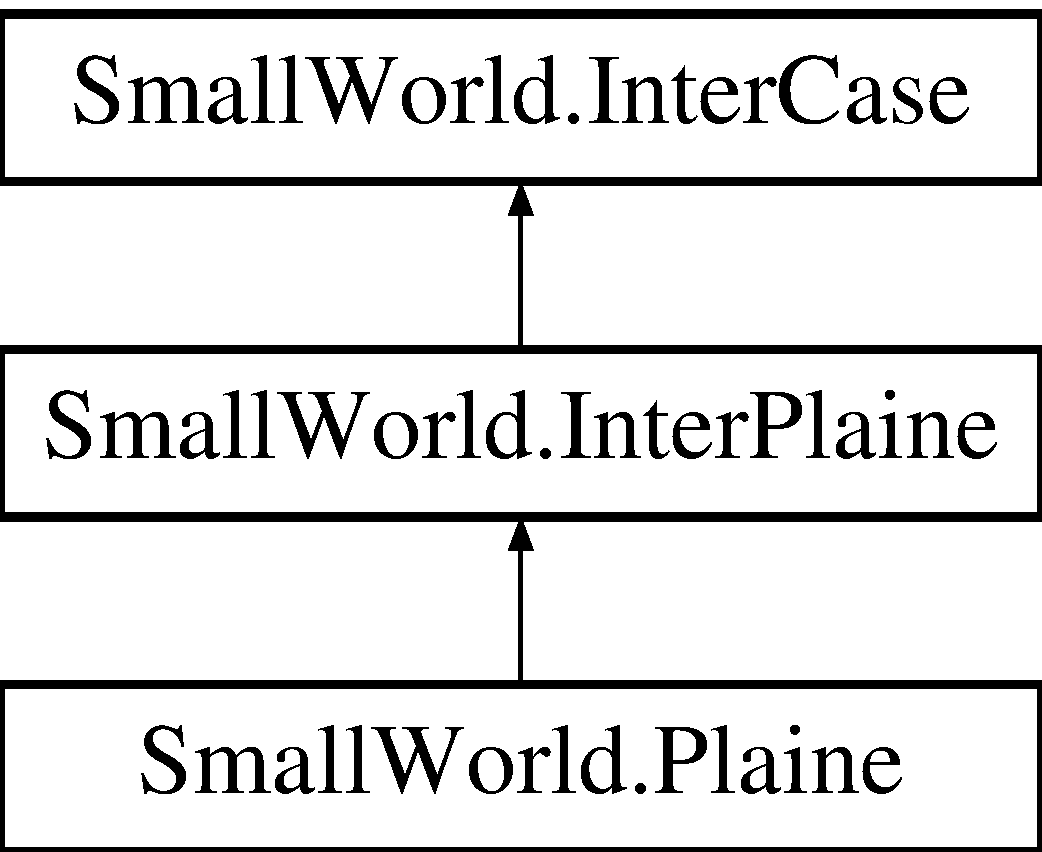
\includegraphics[height=3.000000cm]{interface_small_world_1_1_inter_plaine}
\end{center}
\end{figure}


\subsection{Detailed Description}
Interface pour \hyperlink{class_small_world_1_1_case}{Case} de type plaine. 

The documentation for this interface was generated from the following file\-:\begin{DoxyCompactItemize}
\item 
C\-:/\-Users/damienc/\-Documents/\-Git\-Hub/\-Small\-World/\-Visual\-Studio/\-Projet\-P\-O\-O/\hyperlink{_case_8cs}{Case.\-cs}\end{DoxyCompactItemize}

\hypertarget{interface_small_world_1_1_inter_strategie_carte}{\section{Small\-World.\-Inter\-Strategie\-Carte Interface Reference}
\label{interface_small_world_1_1_inter_strategie_carte}\index{Small\-World.\-Inter\-Strategie\-Carte@{Small\-World.\-Inter\-Strategie\-Carte}}
}
Inheritance diagram for Small\-World.\-Inter\-Strategie\-Carte\-:\begin{figure}[H]
\begin{center}
\leavevmode
\includegraphics[height=1.339713cm]{interface_small_world_1_1_inter_strategie_carte}
\end{center}
\end{figure}
\subsection*{Public Member Functions}
\begin{DoxyCompactItemize}
\item 
void \hyperlink{interface_small_world_1_1_inter_strategie_carte_aa3f0d1267ad71756dc3b134d13733085}{construire} ()
\end{DoxyCompactItemize}


\subsection{Member Function Documentation}
\hypertarget{interface_small_world_1_1_inter_strategie_carte_aa3f0d1267ad71756dc3b134d13733085}{\index{Small\-World\-::\-Inter\-Strategie\-Carte@{Small\-World\-::\-Inter\-Strategie\-Carte}!construire@{construire}}
\index{construire@{construire}!SmallWorld::InterStrategieCarte@{Small\-World\-::\-Inter\-Strategie\-Carte}}
\subsubsection[{construire}]{\setlength{\rightskip}{0pt plus 5cm}void Small\-World.\-Inter\-Strategie\-Carte.\-construire (
\begin{DoxyParamCaption}
{}
\end{DoxyParamCaption}
)}}\label{interface_small_world_1_1_inter_strategie_carte_aa3f0d1267ad71756dc3b134d13733085}


Implemented in \hyperlink{interface_small_world_1_1_inter_strategie_demo_a58c028866f521ee3e50ea0d7e94268e7}{Small\-World.\-Inter\-Strategie\-Demo}, \hyperlink{interface_small_world_1_1_inter_strategie_normale_a6488d973a40d587a3357b6e690104258}{Small\-World.\-Inter\-Strategie\-Normale}, \hyperlink{interface_small_world_1_1_inter_strategie_petite_a41c2fe281215427dbdf531fae8dae05f}{Small\-World.\-Inter\-Strategie\-Petite}, \hyperlink{class_small_world_1_1_strategie_carte_a451fff74bf423f6e225fd4816a7d1868}{Small\-World.\-Strategie\-Carte}, \hyperlink{class_small_world_1_1_strategie_demo_a6a9bbb801d3f894d735dc21d9029c2ee}{Small\-World.\-Strategie\-Demo}, \hyperlink{class_small_world_1_1_strategie_normale_a7f3732b81d0b4b1e11dae277d6db219c}{Small\-World.\-Strategie\-Normale}, and \hyperlink{class_small_world_1_1_strategie_petite_a9ecc5edc2c1d26f7ff8839bea646c698}{Small\-World.\-Strategie\-Petite}.



The documentation for this interface was generated from the following file\-:\begin{DoxyCompactItemize}
\item 
C\-:/\-Users/damienc/\-Documents/\-Git\-Hub/\-Small\-World/\-Visual\-Studio/\-Projet\-P\-O\-O/Carte.\-cs\end{DoxyCompactItemize}

\hypertarget{interface_small_world_1_1_inter_strategie_demo}{\section{Small\-World.\-Inter\-Strategie\-Demo Interface Reference}
\label{interface_small_world_1_1_inter_strategie_demo}\index{Small\-World.\-Inter\-Strategie\-Demo@{Small\-World.\-Inter\-Strategie\-Demo}}
}
Inheritance diagram for Small\-World.\-Inter\-Strategie\-Demo\-:\begin{figure}[H]
\begin{center}
\leavevmode
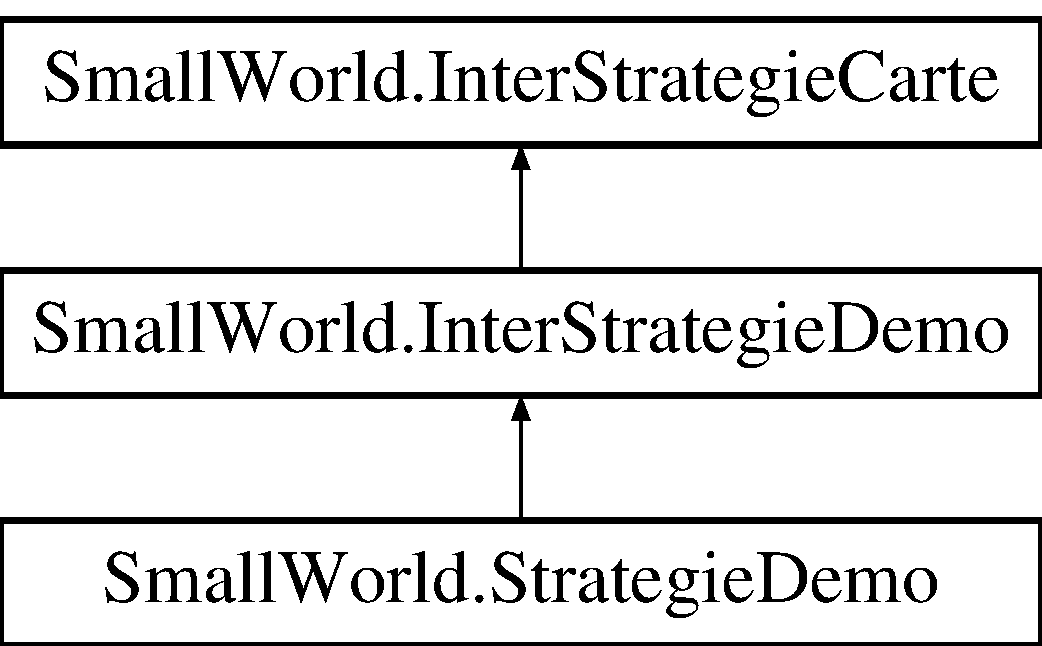
\includegraphics[height=3.000000cm]{interface_small_world_1_1_inter_strategie_demo}
\end{center}
\end{figure}
\subsection*{Public Member Functions}
\begin{DoxyCompactItemize}
\item 
void \hyperlink{interface_small_world_1_1_inter_strategie_demo_a58c028866f521ee3e50ea0d7e94268e7}{construire} ()
\end{DoxyCompactItemize}


\subsection{Member Function Documentation}
\hypertarget{interface_small_world_1_1_inter_strategie_demo_a58c028866f521ee3e50ea0d7e94268e7}{\index{Small\-World\-::\-Inter\-Strategie\-Demo@{Small\-World\-::\-Inter\-Strategie\-Demo}!construire@{construire}}
\index{construire@{construire}!SmallWorld::InterStrategieDemo@{Small\-World\-::\-Inter\-Strategie\-Demo}}
\subsubsection[{construire}]{\setlength{\rightskip}{0pt plus 5cm}void Small\-World.\-Inter\-Strategie\-Demo.\-construire (
\begin{DoxyParamCaption}
{}
\end{DoxyParamCaption}
)}}\label{interface_small_world_1_1_inter_strategie_demo_a58c028866f521ee3e50ea0d7e94268e7}


Implements \hyperlink{interface_small_world_1_1_inter_strategie_carte_aa3f0d1267ad71756dc3b134d13733085}{Small\-World.\-Inter\-Strategie\-Carte}.



Implemented in \hyperlink{class_small_world_1_1_strategie_demo_a6a9bbb801d3f894d735dc21d9029c2ee}{Small\-World.\-Strategie\-Demo}.



The documentation for this interface was generated from the following file\-:\begin{DoxyCompactItemize}
\item 
C\-:/\-Users/damienc/\-Documents/\-Git\-Hub/\-Small\-World/\-Visual\-Studio/\-Projet\-P\-O\-O/Demo.\-cs\end{DoxyCompactItemize}

\hypertarget{interface_small_world_1_1_inter_strategie_normale}{\section{Small\-World.\-Inter\-Strategie\-Normale Interface Reference}
\label{interface_small_world_1_1_inter_strategie_normale}\index{Small\-World.\-Inter\-Strategie\-Normale@{Small\-World.\-Inter\-Strategie\-Normale}}
}


interface pour une stratégie normale  


Inheritance diagram for Small\-World.\-Inter\-Strategie\-Normale\-:\begin{figure}[H]
\begin{center}
\leavevmode
\includegraphics[height=3.000000cm]{interface_small_world_1_1_inter_strategie_normale}
\end{center}
\end{figure}
\subsection*{Public Member Functions}
\begin{DoxyCompactItemize}
\item 
new List$<$ List$<$ \hyperlink{class_small_world_1_1_case}{Case} $>$ $>$ \hyperlink{interface_small_world_1_1_inter_strategie_normale_a98ef2eb599e496422b6ce0e2c1dabad9}{construire} ()
\begin{DoxyCompactList}\small\item\em contruit une carte de taille normale \end{DoxyCompactList}\end{DoxyCompactItemize}


\subsection{Detailed Description}
interface pour une stratégie normale 

\subsection{Member Function Documentation}
\hypertarget{interface_small_world_1_1_inter_strategie_normale_a98ef2eb599e496422b6ce0e2c1dabad9}{\index{Small\-World\-::\-Inter\-Strategie\-Normale@{Small\-World\-::\-Inter\-Strategie\-Normale}!construire@{construire}}
\index{construire@{construire}!SmallWorld::InterStrategieNormale@{Small\-World\-::\-Inter\-Strategie\-Normale}}
\subsubsection[{construire}]{\setlength{\rightskip}{0pt plus 5cm}Small\-World.\-Inter\-Strategie\-Normale.\-construire (
\begin{DoxyParamCaption}
{}
\end{DoxyParamCaption}
)}}\label{interface_small_world_1_1_inter_strategie_normale_a98ef2eb599e496422b6ce0e2c1dabad9}


contruit une carte de taille normale 

\begin{DoxyReturn}{Returns}
la carte demandée 
\end{DoxyReturn}


Implements \hyperlink{interface_small_world_1_1_inter_strategie_carte_aef481b6ecc1f7976bd197147709998b0}{Small\-World.\-Inter\-Strategie\-Carte}.



The documentation for this interface was generated from the following file\-:\begin{DoxyCompactItemize}
\item 
C\-:/\-Users/damienc/\-Documents/\-Git\-Hub/\-Small\-World/\-Visual\-Studio/\-Projet\-P\-O\-O/\hyperlink{_strategie_8cs}{Strategie.\-cs}\end{DoxyCompactItemize}

\hypertarget{interface_small_world_1_1_inter_strategie_petite}{\section{Small\-World.\-Inter\-Strategie\-Petite Interface Reference}
\label{interface_small_world_1_1_inter_strategie_petite}\index{Small\-World.\-Inter\-Strategie\-Petite@{Small\-World.\-Inter\-Strategie\-Petite}}
}
Inheritance diagram for Small\-World.\-Inter\-Strategie\-Petite\-:\begin{figure}[H]
\begin{center}
\leavevmode
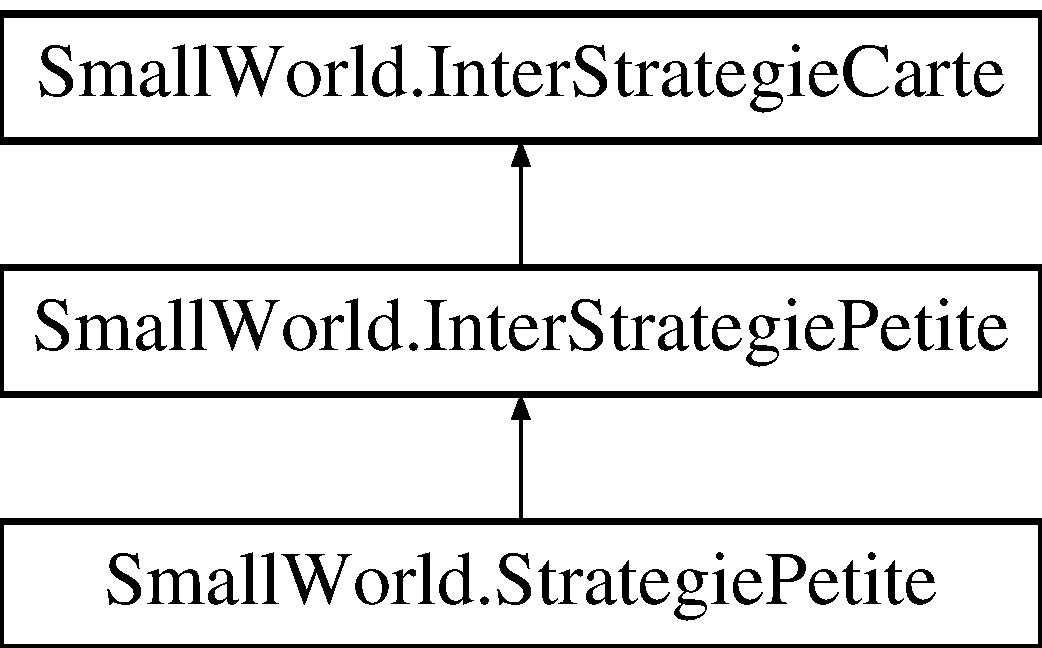
\includegraphics[height=3.000000cm]{interface_small_world_1_1_inter_strategie_petite}
\end{center}
\end{figure}
\subsection*{Public Member Functions}
\begin{DoxyCompactItemize}
\item 
void \hyperlink{interface_small_world_1_1_inter_strategie_petite_a41c2fe281215427dbdf531fae8dae05f}{construire} ()
\end{DoxyCompactItemize}


\subsection{Member Function Documentation}
\hypertarget{interface_small_world_1_1_inter_strategie_petite_a41c2fe281215427dbdf531fae8dae05f}{\index{Small\-World\-::\-Inter\-Strategie\-Petite@{Small\-World\-::\-Inter\-Strategie\-Petite}!construire@{construire}}
\index{construire@{construire}!SmallWorld::InterStrategiePetite@{Small\-World\-::\-Inter\-Strategie\-Petite}}
\subsubsection[{construire}]{\setlength{\rightskip}{0pt plus 5cm}void Small\-World.\-Inter\-Strategie\-Petite.\-construire (
\begin{DoxyParamCaption}
{}
\end{DoxyParamCaption}
)}}\label{interface_small_world_1_1_inter_strategie_petite_a41c2fe281215427dbdf531fae8dae05f}


Implements \hyperlink{interface_small_world_1_1_inter_strategie_carte_aa3f0d1267ad71756dc3b134d13733085}{Small\-World.\-Inter\-Strategie\-Carte}.



Implemented in \hyperlink{class_small_world_1_1_strategie_petite_a9ecc5edc2c1d26f7ff8839bea646c698}{Small\-World.\-Strategie\-Petite}.



The documentation for this interface was generated from the following file\-:\begin{DoxyCompactItemize}
\item 
C\-:/\-Users/damienc/\-Documents/\-Git\-Hub/\-Small\-World/\-Visual\-Studio/\-Projet\-P\-O\-O/Petite.\-cs\end{DoxyCompactItemize}

\hypertarget{interface_small_world_1_1_inter_unite}{\section{Small\-World.\-Inter\-Unite Interface Reference}
\label{interface_small_world_1_1_inter_unite}\index{Small\-World.\-Inter\-Unite@{Small\-World.\-Inter\-Unite}}
}
Inheritance diagram for Small\-World.\-Inter\-Unite\-:\begin{figure}[H]
\begin{center}
\leavevmode
\includegraphics[height=1.481482cm]{interface_small_world_1_1_inter_unite}
\end{center}
\end{figure}
\subsection*{Public Member Functions}
\begin{DoxyCompactItemize}
\item 
\hypertarget{interface_small_world_1_1_inter_unite_a1a5d372f4b0e3df0729649ea0ffef763}{void {\bfseries attaquer} ()}\label{interface_small_world_1_1_inter_unite_a1a5d372f4b0e3df0729649ea0ffef763}

\item 
\hypertarget{interface_small_world_1_1_inter_unite_a56e9c8df0434d82d009cba43ebfebed5}{void {\bfseries deplacer} ()}\label{interface_small_world_1_1_inter_unite_a56e9c8df0434d82d009cba43ebfebed5}

\end{DoxyCompactItemize}


The documentation for this interface was generated from the following file\-:\begin{DoxyCompactItemize}
\item 
C\-:/\-Users/damienc/\-Documents/\-Git\-Hub/\-Small\-World/\-Visual\-Studio/\-Projet\-P\-O\-O/Unite.\-cs\end{DoxyCompactItemize}

\hypertarget{interface_small_world_1_1_inter_unite_gauloise}{\section{Small\-World.\-Inter\-Unite\-Gauloise Interface Reference}
\label{interface_small_world_1_1_inter_unite_gauloise}\index{Small\-World.\-Inter\-Unite\-Gauloise@{Small\-World.\-Inter\-Unite\-Gauloise}}
}


Interface pour les unités gauloises.  


Inheritance diagram for Small\-World.\-Inter\-Unite\-Gauloise\-:\begin{figure}[H]
\begin{center}
\leavevmode
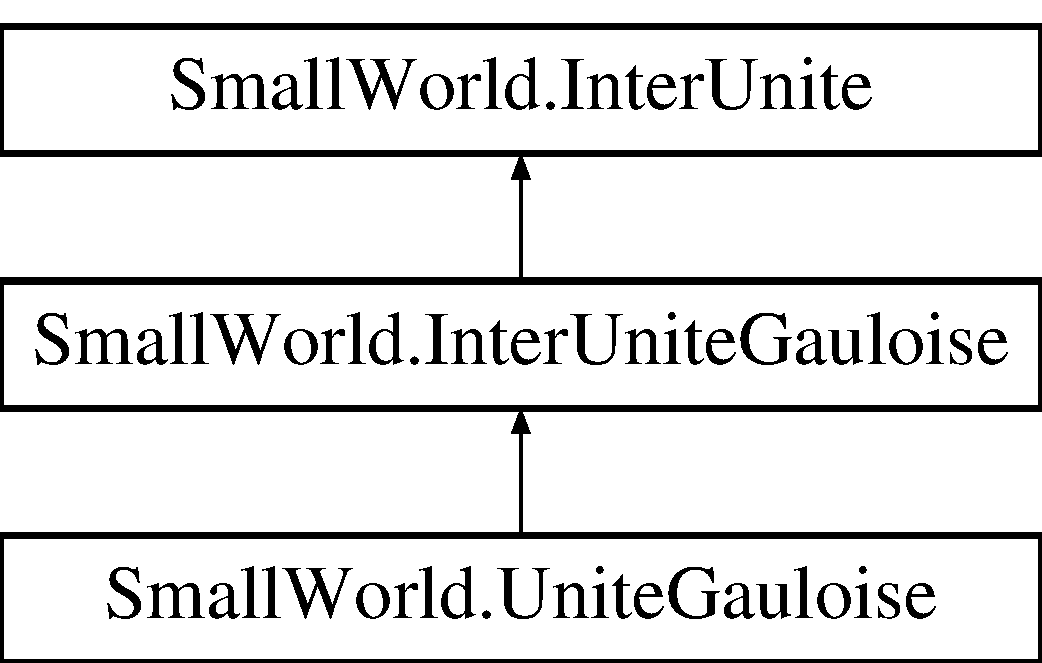
\includegraphics[height=3.000000cm]{interface_small_world_1_1_inter_unite_gauloise}
\end{center}
\end{figure}
\subsection*{Additional Inherited Members}


\subsection{Detailed Description}
Interface pour les unités gauloises. 

The documentation for this interface was generated from the following file\-:\begin{DoxyCompactItemize}
\item 
C\-:/\-Users/damienc/\-Documents/\-Git\-Hub/\-Small\-World/\-Visual\-Studio/\-Projet\-P\-O\-O/\hyperlink{_unite_8cs}{Unite.\-cs}\end{DoxyCompactItemize}

\hypertarget{interface_small_world_1_1_inter_unite_naine}{\section{Small\-World.\-Inter\-Unite\-Naine Interface Reference}
\label{interface_small_world_1_1_inter_unite_naine}\index{Small\-World.\-Inter\-Unite\-Naine@{Small\-World.\-Inter\-Unite\-Naine}}
}


Interface pour les unités naines.  


Inheritance diagram for Small\-World.\-Inter\-Unite\-Naine\-:\begin{figure}[H]
\begin{center}
\leavevmode
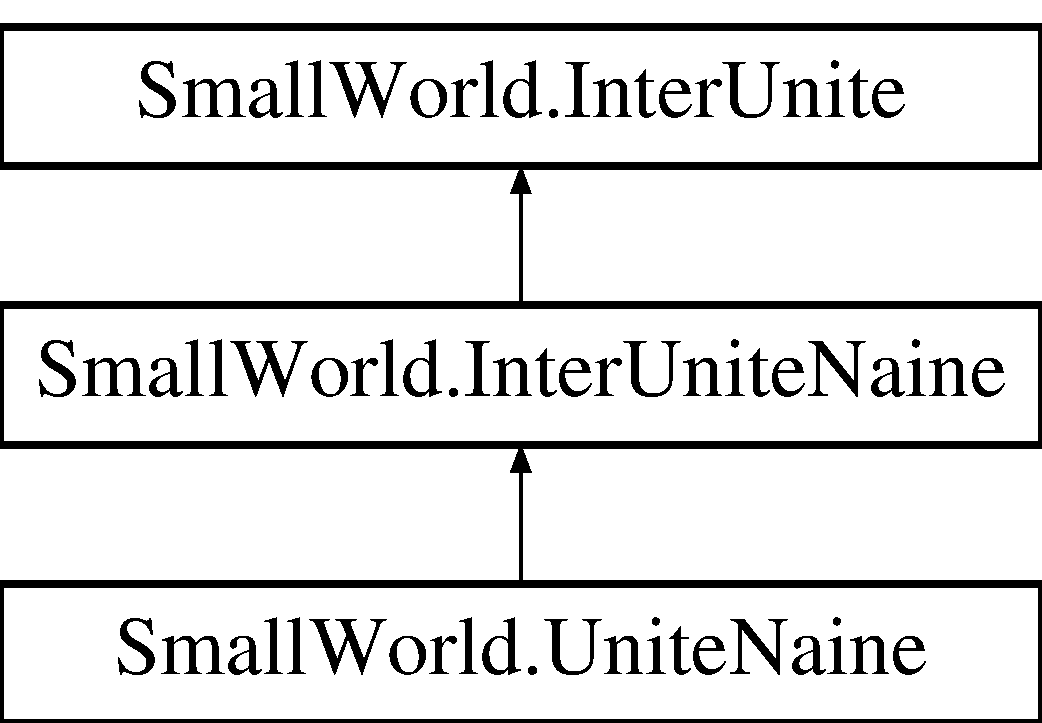
\includegraphics[height=3.000000cm]{interface_small_world_1_1_inter_unite_naine}
\end{center}
\end{figure}
\subsection*{Additional Inherited Members}


\subsection{Detailed Description}
Interface pour les unités naines. 

The documentation for this interface was generated from the following file\-:\begin{DoxyCompactItemize}
\item 
C\-:/\-Users/damienc/\-Documents/\-Git\-Hub/\-Small\-World/\-Visual\-Studio/\-Projet\-P\-O\-O/\hyperlink{_unite_8cs}{Unite.\-cs}\end{DoxyCompactItemize}

\hypertarget{interface_small_world_1_1_inter_unite_viking}{\section{Small\-World.\-Inter\-Unite\-Viking Interface Reference}
\label{interface_small_world_1_1_inter_unite_viking}\index{Small\-World.\-Inter\-Unite\-Viking@{Small\-World.\-Inter\-Unite\-Viking}}
}


Interface pour les unités viking.  


Inheritance diagram for Small\-World.\-Inter\-Unite\-Viking\-:\begin{figure}[H]
\begin{center}
\leavevmode
\includegraphics[height=3.000000cm]{interface_small_world_1_1_inter_unite_viking}
\end{center}
\end{figure}
\subsection*{Additional Inherited Members}


\subsection{Detailed Description}
Interface pour les unités viking. 

The documentation for this interface was generated from the following file\-:\begin{DoxyCompactItemize}
\item 
C\-:/\-Users/damienc/\-Documents/\-Git\-Hub/\-Small\-World/\-Visual\-Studio/\-Projet\-P\-O\-O/\hyperlink{_unite_8cs}{Unite.\-cs}\end{DoxyCompactItemize}

\hypertarget{class_small_world_1_1_joueur}{\section{Small\-World.\-Joueur Class Reference}
\label{class_small_world_1_1_joueur}\index{Small\-World.\-Joueur@{Small\-World.\-Joueur}}
}
Inheritance diagram for Small\-World.\-Joueur\-:\begin{figure}[H]
\begin{center}
\leavevmode
\includegraphics[height=2.000000cm]{class_small_world_1_1_joueur}
\end{center}
\end{figure}
\subsection*{Public Member Functions}
\begin{DoxyCompactItemize}
\item 
\hypertarget{class_small_world_1_1_joueur_a7e0f92b4b3a20dd86dabb9a2c986dcc0}{void {\bfseries calculer\-Point\-Victoire} ()}\label{class_small_world_1_1_joueur_a7e0f92b4b3a20dd86dabb9a2c986dcc0}

\item 
\hypertarget{class_small_world_1_1_joueur_a9fa34909f3b3614fe95a6e9e658f326d}{void {\bfseries creer\-Joueur} ()}\label{class_small_world_1_1_joueur_a9fa34909f3b3614fe95a6e9e658f326d}

\end{DoxyCompactItemize}
\subsection*{Properties}
\begin{DoxyCompactItemize}
\item 
\hypertarget{class_small_world_1_1_joueur_aa067290a5f303e61a281cef9be45616e}{\hyperlink{class_small_world_1_1_unite}{Unite} {\bfseries unite}\hspace{0.3cm}{\ttfamily  \mbox{[}get, set\mbox{]}}}\label{class_small_world_1_1_joueur_aa067290a5f303e61a281cef9be45616e}

\item 
\hypertarget{class_small_world_1_1_joueur_aaedc71c4e752242d027683df8f7d4ec1}{\hyperlink{class_small_world_1_1_peuple}{Peuple} {\bfseries peuple}\hspace{0.3cm}{\ttfamily  \mbox{[}get, set\mbox{]}}}\label{class_small_world_1_1_joueur_aaedc71c4e752242d027683df8f7d4ec1}

\item 
\hypertarget{class_small_world_1_1_joueur_a90b37fe50d88159251b64d456c8998f0}{int {\bfseries point\-Victoire}\hspace{0.3cm}{\ttfamily  \mbox{[}get, set\mbox{]}}}\label{class_small_world_1_1_joueur_a90b37fe50d88159251b64d456c8998f0}

\end{DoxyCompactItemize}


The documentation for this class was generated from the following file\-:\begin{DoxyCompactItemize}
\item 
C\-:/\-Users/damienc/\-Documents/\-Git\-Hub/\-Small\-World/\-Visual\-Studio/\-Projet\-P\-O\-O/Joueur.\-cs\end{DoxyCompactItemize}

\hypertarget{class_small_world_1_1_montagne}{\section{Small\-World.\-Montagne Class Reference}
\label{class_small_world_1_1_montagne}\index{Small\-World.\-Montagne@{Small\-World.\-Montagne}}
}
Inheritance diagram for Small\-World.\-Montagne\-:\begin{figure}[H]
\begin{center}
\leavevmode
\includegraphics[height=3.000000cm]{class_small_world_1_1_montagne}
\end{center}
\end{figure}
\subsection*{Additional Inherited Members}


The documentation for this class was generated from the following file\-:\begin{DoxyCompactItemize}
\item 
C\-:/\-Users/damienc/\-Documents/\-Git\-Hub/\-Small\-World/\-Visual\-Studio/\-Projet\-P\-O\-O/Case.\-cs\end{DoxyCompactItemize}

\hypertarget{class_small_world_1_1_monteur_partie}{\section{Small\-World.\-Monteur\-Partie Class Reference}
\label{class_small_world_1_1_monteur_partie}\index{Small\-World.\-Monteur\-Partie@{Small\-World.\-Monteur\-Partie}}
}


Classe abstraite implémentant Inter\-Monteur \hyperlink{interface_small_world_1_1_inter_partie}{Inter\-Partie}.  


Inheritance diagram for Small\-World.\-Monteur\-Partie\-:\begin{figure}[H]
\begin{center}
\leavevmode
\includegraphics[height=2.616822cm]{class_small_world_1_1_monteur_partie}
\end{center}
\end{figure}
\subsection*{Public Member Functions}
\begin{DoxyCompactItemize}
\item 
void \hyperlink{class_small_world_1_1_monteur_partie_ad8cedb326193c0f0ff5f2d6705867156}{ajouter\-Carte} ()
\begin{DoxyCompactList}\small\item\em Ajout de la carte pour la construction d'une partie. \end{DoxyCompactList}\item 
void \hyperlink{class_small_world_1_1_monteur_partie_ac1e20f04d1ca796c1aa0ab504ecb1d2a}{ajouter\-Joueur} (string nom\-Joueur, string peuple)
\begin{DoxyCompactList}\small\item\em Ajout d'un joueur. \end{DoxyCompactList}\item 
\hyperlink{class_small_world_1_1_partie}{Partie} \hyperlink{class_small_world_1_1_monteur_partie_a76b953c2a45b0c3355d764355d85e225}{creer\-Partie} (string nom\-Joueur\-A, string peuple\-A, string nom\-Joueur\-B, string peuple\-B)
\begin{DoxyCompactList}\small\item\em Création de la partie. \end{DoxyCompactList}\item 
void \hyperlink{class_small_world_1_1_monteur_partie_a8bfe459f9efcb0561a7612e720e0a373}{initialiser\-Nombre\-Tour} ()
\begin{DoxyCompactList}\small\item\em initialise le nombre de tour d'un partie \end{DoxyCompactList}\item 
unsafe void \hyperlink{class_small_world_1_1_monteur_partie_a5cba1ab3dd04f490331bf22e540cc80e}{placer\-Unites} ()
\begin{DoxyCompactList}\small\item\em Place le nombre d'unité nécessaire au début de la partie. \end{DoxyCompactList}\end{DoxyCompactItemize}
\subsection*{Protected Attributes}
\begin{DoxyCompactItemize}
\item 
\hypertarget{class_small_world_1_1_monteur_partie_a44a0c5d06ba0529da7ded15eeae110b0}{int \hyperlink{class_small_world_1_1_monteur_partie_a44a0c5d06ba0529da7ded15eeae110b0}{nb\-\_\-case}}\label{class_small_world_1_1_monteur_partie_a44a0c5d06ba0529da7ded15eeae110b0}

\begin{DoxyCompactList}\small\item\em constante {\bfseries nb\-\_\-case} le nombre initial de tour \end{DoxyCompactList}\item 
\hypertarget{class_small_world_1_1_monteur_partie_a063951c1b42071c88f4354541ac31dfc}{int \hyperlink{class_small_world_1_1_monteur_partie_a063951c1b42071c88f4354541ac31dfc}{nb\-\_\-tour}}\label{class_small_world_1_1_monteur_partie_a063951c1b42071c88f4354541ac31dfc}

\begin{DoxyCompactList}\small\item\em constante {\bfseries nb\-\_\-tour} le nombre initial de tour \end{DoxyCompactList}\item 
\hypertarget{class_small_world_1_1_monteur_partie_a051496e5be6c5f21de6519605ea4c5a7}{int \hyperlink{class_small_world_1_1_monteur_partie_a051496e5be6c5f21de6519605ea4c5a7}{nb\-\_\-unite}}\label{class_small_world_1_1_monteur_partie_a051496e5be6c5f21de6519605ea4c5a7}

\begin{DoxyCompactList}\small\item\em constante {\bfseries nb\-\_\-unite} le nombre initial d'unité par joueur \end{DoxyCompactList}\end{DoxyCompactItemize}
\subsection*{Properties}
\begin{DoxyCompactItemize}
\item 
\hypertarget{class_small_world_1_1_monteur_partie_a1ec639225ca9a5bb10cd3ea3d76820c7}{int {\bfseries Nb\-\_\-case}\hspace{0.3cm}{\ttfamily  \mbox{[}get\mbox{]}}}\label{class_small_world_1_1_monteur_partie_a1ec639225ca9a5bb10cd3ea3d76820c7}

\item 
\hypertarget{class_small_world_1_1_monteur_partie_af44a6f3594947ce5647ecb63991e1088}{int \hyperlink{class_small_world_1_1_monteur_partie_af44a6f3594947ce5647ecb63991e1088}{Nb\-\_\-tour}\hspace{0.3cm}{\ttfamily  \mbox{[}get\mbox{]}}}\label{class_small_world_1_1_monteur_partie_af44a6f3594947ce5647ecb63991e1088}

\begin{DoxyCompactList}\small\item\em \hyperlink{namespace_small_world_1_1_properties}{Properties} pour l'attribut nb\-\_\-tour. \end{DoxyCompactList}\item 
\hypertarget{class_small_world_1_1_monteur_partie_a5469de7a7a7e109b9ef8d2663d2f1f04}{int \hyperlink{class_small_world_1_1_monteur_partie_a5469de7a7a7e109b9ef8d2663d2f1f04}{Nb\-\_\-unite}\hspace{0.3cm}{\ttfamily  \mbox{[}get\mbox{]}}}\label{class_small_world_1_1_monteur_partie_a5469de7a7a7e109b9ef8d2663d2f1f04}

\begin{DoxyCompactList}\small\item\em \hyperlink{namespace_small_world_1_1_properties}{Properties} pour l'attribut nb\-\_\-unite. \end{DoxyCompactList}\item 
\hypertarget{class_small_world_1_1_monteur_partie_abf37bc99734d517060ee5a86f41abc96}{\hyperlink{class_small_world_1_1_fabrique_peuple}{Fabrique\-Peuple} \hyperlink{class_small_world_1_1_monteur_partie_abf37bc99734d517060ee5a86f41abc96}{Fabrique\-Peuple}\hspace{0.3cm}{\ttfamily  \mbox{[}get, set\mbox{]}}}\label{class_small_world_1_1_monteur_partie_abf37bc99734d517060ee5a86f41abc96}

\begin{DoxyCompactList}\small\item\em \hyperlink{namespace_small_world_1_1_properties}{Properties} pour l'attribut fabrique\-Peuple. \end{DoxyCompactList}\item 
\hypertarget{class_small_world_1_1_monteur_partie_a9591641b71bf77ba0c67110989202da0}{\hyperlink{class_small_world_1_1_partie}{Partie} \hyperlink{class_small_world_1_1_monteur_partie_a9591641b71bf77ba0c67110989202da0}{Partie}\hspace{0.3cm}{\ttfamily  \mbox{[}get, set\mbox{]}}}\label{class_small_world_1_1_monteur_partie_a9591641b71bf77ba0c67110989202da0}

\begin{DoxyCompactList}\small\item\em \hyperlink{namespace_small_world_1_1_properties}{Properties} pour l'attribut partie. \end{DoxyCompactList}\item 
\hypertarget{class_small_world_1_1_monteur_partie_a4fa6b0de5f3b2ff1e10756300e6b1654}{\hyperlink{class_small_world_1_1_carte}{Carte} \hyperlink{class_small_world_1_1_monteur_partie_a4fa6b0de5f3b2ff1e10756300e6b1654}{Carte}\hspace{0.3cm}{\ttfamily  \mbox{[}get, set\mbox{]}}}\label{class_small_world_1_1_monteur_partie_a4fa6b0de5f3b2ff1e10756300e6b1654}

\begin{DoxyCompactList}\small\item\em \hyperlink{namespace_small_world_1_1_properties}{Properties} pour l'attribut carte. \end{DoxyCompactList}\item 
\hypertarget{class_small_world_1_1_monteur_partie_ac7f1bc160be378d8dcae1cb00d86f312}{\hyperlink{class_small_world_1_1_strategie_carte}{Strategie\-Carte} \hyperlink{class_small_world_1_1_monteur_partie_ac7f1bc160be378d8dcae1cb00d86f312}{Strategie}\hspace{0.3cm}{\ttfamily  \mbox{[}get, set\mbox{]}}}\label{class_small_world_1_1_monteur_partie_ac7f1bc160be378d8dcae1cb00d86f312}

\begin{DoxyCompactList}\small\item\em \hyperlink{namespace_small_world_1_1_properties}{Properties} pour l'attribut strategie. \end{DoxyCompactList}\end{DoxyCompactItemize}


\subsection{Detailed Description}
Classe abstraite implémentant Inter\-Monteur \hyperlink{interface_small_world_1_1_inter_partie}{Inter\-Partie}. 

\subsection{Member Function Documentation}
\hypertarget{class_small_world_1_1_monteur_partie_ad8cedb326193c0f0ff5f2d6705867156}{\index{Small\-World\-::\-Monteur\-Partie@{Small\-World\-::\-Monteur\-Partie}!ajouter\-Carte@{ajouter\-Carte}}
\index{ajouter\-Carte@{ajouter\-Carte}!SmallWorld::MonteurPartie@{Small\-World\-::\-Monteur\-Partie}}
\subsubsection[{ajouter\-Carte}]{\setlength{\rightskip}{0pt plus 5cm}Small\-World.\-Monteur\-Partie.\-ajouter\-Carte (
\begin{DoxyParamCaption}
{}
\end{DoxyParamCaption}
)}}\label{class_small_world_1_1_monteur_partie_ad8cedb326193c0f0ff5f2d6705867156}


Ajout de la carte pour la construction d'une partie. 

\begin{DoxyReturn}{Returns}
void 
\end{DoxyReturn}


Implements \hyperlink{interface_small_world_1_1_inter_monteur_partie_a473c91ad26ee485f07261df1fcae0e8b}{Small\-World.\-Inter\-Monteur\-Partie}.

\hypertarget{class_small_world_1_1_monteur_partie_ac1e20f04d1ca796c1aa0ab504ecb1d2a}{\index{Small\-World\-::\-Monteur\-Partie@{Small\-World\-::\-Monteur\-Partie}!ajouter\-Joueur@{ajouter\-Joueur}}
\index{ajouter\-Joueur@{ajouter\-Joueur}!SmallWorld::MonteurPartie@{Small\-World\-::\-Monteur\-Partie}}
\subsubsection[{ajouter\-Joueur}]{\setlength{\rightskip}{0pt plus 5cm}Small\-World.\-Monteur\-Partie.\-ajouter\-Joueur (
\begin{DoxyParamCaption}
\item[{string}]{nom\-Joueur, }
\item[{string}]{peuple}
\end{DoxyParamCaption}
)}}\label{class_small_world_1_1_monteur_partie_ac1e20f04d1ca796c1aa0ab504ecb1d2a}


Ajout d'un joueur. 


\begin{DoxyParams}{Parameters}
{\em string} & {\bfseries nom\-Joueur} le nom du joueur \\
\hline
{\em string} & {\bfseries peuple} le type de peuple \\
\hline
\end{DoxyParams}
\begin{DoxyReturn}{Returns}
void 
\end{DoxyReturn}


Implements \hyperlink{interface_small_world_1_1_inter_monteur_partie_ae52498262dd36230b0c0d090cb59ff07}{Small\-World.\-Inter\-Monteur\-Partie}.

\hypertarget{class_small_world_1_1_monteur_partie_a76b953c2a45b0c3355d764355d85e225}{\index{Small\-World\-::\-Monteur\-Partie@{Small\-World\-::\-Monteur\-Partie}!creer\-Partie@{creer\-Partie}}
\index{creer\-Partie@{creer\-Partie}!SmallWorld::MonteurPartie@{Small\-World\-::\-Monteur\-Partie}}
\subsubsection[{creer\-Partie}]{\setlength{\rightskip}{0pt plus 5cm}Small\-World.\-Monteur\-Partie.\-creer\-Partie (
\begin{DoxyParamCaption}
\item[{string}]{nom\-Joueur\-A, }
\item[{string}]{peuple\-A, }
\item[{string}]{nom\-Joueur\-B, }
\item[{string}]{peuple\-B}
\end{DoxyParamCaption}
)}}\label{class_small_world_1_1_monteur_partie_a76b953c2a45b0c3355d764355d85e225}


Création de la partie. 


\begin{DoxyParams}{Parameters}
{\em string} & {\bfseries nom\-Joueur\-A} le nom du premier joueur \\
\hline
{\em string} & {\bfseries peuple\-A} le peuple du premier joueur \\
\hline
{\em string} & {\bfseries nom\-Joueur\-B} le nom du deuxième joueur \\
\hline
{\em string} & {\bfseries peuple\-B} le peuple du deuxième joueur \\
\hline
\end{DoxyParams}
\begin{DoxyReturn}{Returns}
\hyperlink{class_small_world_1_1_partie}{Partie} la nouvelle partie 
\end{DoxyReturn}


Implements \hyperlink{interface_small_world_1_1_inter_monteur_partie_ad471ab6610aaa1664fb3d0bd93f00be3}{Small\-World.\-Inter\-Monteur\-Partie}.

\hypertarget{class_small_world_1_1_monteur_partie_a8bfe459f9efcb0561a7612e720e0a373}{\index{Small\-World\-::\-Monteur\-Partie@{Small\-World\-::\-Monteur\-Partie}!initialiser\-Nombre\-Tour@{initialiser\-Nombre\-Tour}}
\index{initialiser\-Nombre\-Tour@{initialiser\-Nombre\-Tour}!SmallWorld::MonteurPartie@{Small\-World\-::\-Monteur\-Partie}}
\subsubsection[{initialiser\-Nombre\-Tour}]{\setlength{\rightskip}{0pt plus 5cm}Small\-World.\-Monteur\-Partie.\-initialiser\-Nombre\-Tour (
\begin{DoxyParamCaption}
{}
\end{DoxyParamCaption}
)}}\label{class_small_world_1_1_monteur_partie_a8bfe459f9efcb0561a7612e720e0a373}


initialise le nombre de tour d'un partie 

\begin{DoxyReturn}{Returns}
void 
\end{DoxyReturn}


Implements \hyperlink{interface_small_world_1_1_inter_monteur_partie_afa1b718338a15b4dd0deb5d817f3484c}{Small\-World.\-Inter\-Monteur\-Partie}.

\hypertarget{class_small_world_1_1_monteur_partie_a5cba1ab3dd04f490331bf22e540cc80e}{\index{Small\-World\-::\-Monteur\-Partie@{Small\-World\-::\-Monteur\-Partie}!placer\-Unites@{placer\-Unites}}
\index{placer\-Unites@{placer\-Unites}!SmallWorld::MonteurPartie@{Small\-World\-::\-Monteur\-Partie}}
\subsubsection[{placer\-Unites}]{\setlength{\rightskip}{0pt plus 5cm}Small\-World.\-Monteur\-Partie.\-placer\-Unites (
\begin{DoxyParamCaption}
{}
\end{DoxyParamCaption}
)}}\label{class_small_world_1_1_monteur_partie_a5cba1ab3dd04f490331bf22e540cc80e}


Place le nombre d'unité nécessaire au début de la partie. 

\begin{DoxyReturn}{Returns}
void 
\end{DoxyReturn}


Implements \hyperlink{interface_small_world_1_1_inter_monteur_partie_a4ea7442b592d23a0f31e0d0020f124de}{Small\-World.\-Inter\-Monteur\-Partie}.



The documentation for this class was generated from the following file\-:\begin{DoxyCompactItemize}
\item 
C\-:/\-Users/damienc/\-Documents/\-Git\-Hub/\-Small\-World/\-Visual\-Studio/\-Projet\-P\-O\-O/\hyperlink{_monteur_partie_8cs}{Monteur\-Partie.\-cs}\end{DoxyCompactItemize}

\hypertarget{class_small_world_1_1_monteur_partie_demo}{\section{Small\-World.\-Monteur\-Partie\-Demo Class Reference}
\label{class_small_world_1_1_monteur_partie_demo}\index{Small\-World.\-Monteur\-Partie\-Demo@{Small\-World.\-Monteur\-Partie\-Demo}}
}


classe pour un monteur d'une partie démo  


Inheritance diagram for Small\-World.\-Monteur\-Partie\-Demo\-:\begin{figure}[H]
\begin{center}
\leavevmode
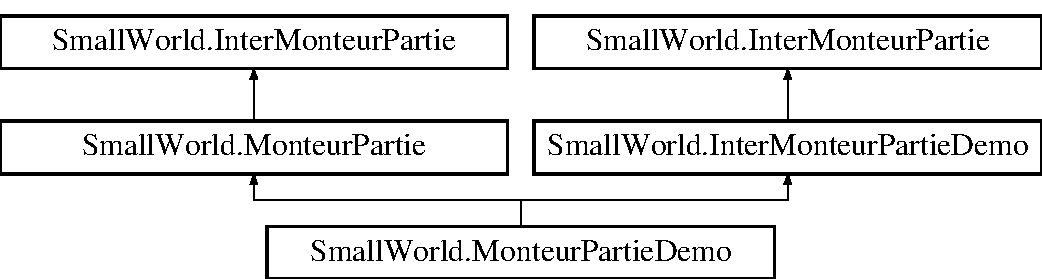
\includegraphics[height=3.000000cm]{class_small_world_1_1_monteur_partie_demo}
\end{center}
\end{figure}
\subsection*{Public Member Functions}
\begin{DoxyCompactItemize}
\item 
\hypertarget{class_small_world_1_1_monteur_partie_demo_aad8fb3b06db6f02910dbb256d2233a0a}{\hyperlink{class_small_world_1_1_monteur_partie_demo_aad8fb3b06db6f02910dbb256d2233a0a}{Monteur\-Partie\-Demo} ()}\label{class_small_world_1_1_monteur_partie_demo_aad8fb3b06db6f02910dbb256d2233a0a}

\begin{DoxyCompactList}\small\item\em Constructeur d'un \hyperlink{class_small_world_1_1_monteur_partie_demo}{Monteur\-Partie\-Demo}. \end{DoxyCompactList}\end{DoxyCompactItemize}
\subsection*{Additional Inherited Members}


\subsection{Detailed Description}
classe pour un monteur d'une partie démo 

The documentation for this class was generated from the following file\-:\begin{DoxyCompactItemize}
\item 
C\-:/\-Users/damienc/\-Documents/\-Git\-Hub/\-Small\-World/\-Visual\-Studio/\-Projet\-P\-O\-O/\hyperlink{_monteur_partie_8cs}{Monteur\-Partie.\-cs}\end{DoxyCompactItemize}

\hypertarget{class_small_world_1_1_monteur_partie_normale}{\section{Small\-World.\-Monteur\-Partie\-Normale Class Reference}
\label{class_small_world_1_1_monteur_partie_normale}\index{Small\-World.\-Monteur\-Partie\-Normale@{Small\-World.\-Monteur\-Partie\-Normale}}
}
Inheritance diagram for Small\-World.\-Monteur\-Partie\-Normale\-:\begin{figure}[H]
\begin{center}
\leavevmode
\includegraphics[height=2.343096cm]{class_small_world_1_1_monteur_partie_normale}
\end{center}
\end{figure}
\subsection*{Public Member Functions}
\begin{DoxyCompactItemize}
\item 
\hypertarget{class_small_world_1_1_monteur_partie_normale_a095529a4b08f7227415e960e7edf4be4}{void {\bfseries ajouter\-Peuple} ()}\label{class_small_world_1_1_monteur_partie_normale_a095529a4b08f7227415e960e7edf4be4}

\item 
\hypertarget{class_small_world_1_1_monteur_partie_normale_a27f7e7f429852ea6f543593d09b31f93}{\hyperlink{interface_small_world_1_1_partie}{Small\-World.\-Partie} \hyperlink{class_small_world_1_1_monteur_partie_normale_a27f7e7f429852ea6f543593d09b31f93}{creer\-Partie} ()}\label{class_small_world_1_1_monteur_partie_normale_a27f7e7f429852ea6f543593d09b31f93}

\begin{DoxyCompactList}\small\item\em Création la partie. \end{DoxyCompactList}\item 
\hypertarget{class_small_world_1_1_monteur_partie_normale_a9f6a6e1e348fa3d971ee8a409e986c55}{void {\bfseries ajouter\-Carte} ()}\label{class_small_world_1_1_monteur_partie_normale_a9f6a6e1e348fa3d971ee8a409e986c55}

\item 
\hypertarget{class_small_world_1_1_monteur_partie_normale_a6ba30a3502a862c7943ba991eacc2fb0}{void {\bfseries ajouter\-Joueur} ()}\label{class_small_world_1_1_monteur_partie_normale_a6ba30a3502a862c7943ba991eacc2fb0}

\item 
\hypertarget{class_small_world_1_1_monteur_partie_normale_a79b156ac66696c5bce20cb025a39f1ce}{void \hyperlink{class_small_world_1_1_monteur_partie_normale_a79b156ac66696c5bce20cb025a39f1ce}{placer\-Unites} ()}\label{class_small_world_1_1_monteur_partie_normale_a79b156ac66696c5bce20cb025a39f1ce}

\begin{DoxyCompactList}\small\item\em Placement des unités avant le début de la partie. \end{DoxyCompactList}\end{DoxyCompactItemize}


The documentation for this class was generated from the following file\-:\begin{DoxyCompactItemize}
\item 
C\-:/\-Users/damienc/\-Documents/\-Git\-Hub/\-Small\-World/\-Visual\-Studio/\-Projet\-P\-O\-O/\hyperlink{_monteur_partie_8cs}{Monteur\-Partie.\-cs}\end{DoxyCompactItemize}

\hypertarget{class_small_world_1_1_monteur_partie_petite}{\section{Small\-World.\-Monteur\-Partie\-Petite Class Reference}
\label{class_small_world_1_1_monteur_partie_petite}\index{Small\-World.\-Monteur\-Partie\-Petite@{Small\-World.\-Monteur\-Partie\-Petite}}
}


classe pour un monteur d'une partie petite  


Inheritance diagram for Small\-World.\-Monteur\-Partie\-Petite\-:\begin{figure}[H]
\begin{center}
\leavevmode
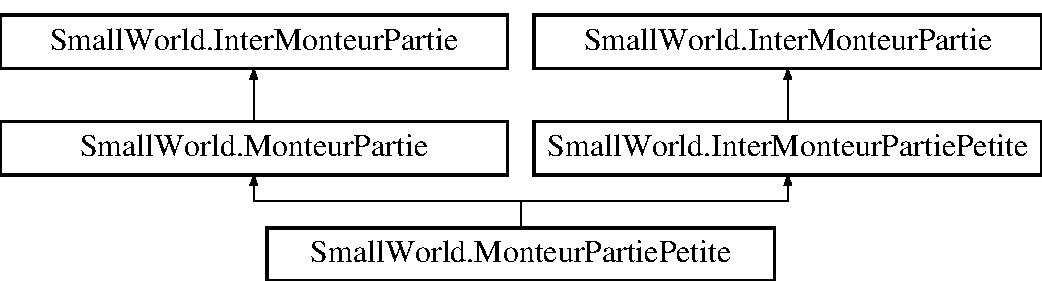
\includegraphics[height=3.000000cm]{class_small_world_1_1_monteur_partie_petite}
\end{center}
\end{figure}
\subsection*{Public Member Functions}
\begin{DoxyCompactItemize}
\item 
\hypertarget{class_small_world_1_1_monteur_partie_petite_a9241a473b8a823da6141e9be321216a8}{\hyperlink{class_small_world_1_1_monteur_partie_petite_a9241a473b8a823da6141e9be321216a8}{Monteur\-Partie\-Petite} ()}\label{class_small_world_1_1_monteur_partie_petite_a9241a473b8a823da6141e9be321216a8}

\begin{DoxyCompactList}\small\item\em Constructeur d'un \hyperlink{class_small_world_1_1_monteur_partie_petite}{Monteur\-Partie\-Petite}. \end{DoxyCompactList}\end{DoxyCompactItemize}
\subsection*{Additional Inherited Members}


\subsection{Detailed Description}
classe pour un monteur d'une partie petite 

The documentation for this class was generated from the following file\-:\begin{DoxyCompactItemize}
\item 
C\-:/\-Users/damienc/\-Documents/\-Git\-Hub/\-Small\-World/\-Visual\-Studio/\-Projet\-P\-O\-O/\hyperlink{_monteur_partie_8cs}{Monteur\-Partie.\-cs}\end{DoxyCompactItemize}

\hypertarget{interface_small_world_1_1_nain}{\section{Small\-World.\-Nain Interface Reference}
\label{interface_small_world_1_1_nain}\index{Small\-World.\-Nain@{Small\-World.\-Nain}}
}


The documentation for this interface was generated from the following file\-:\begin{DoxyCompactItemize}
\item 
C\-:/\-Users/damienc/\-Documents/\-Git\-Hub/\-Small\-World/\-Visual\-Studio/\-Projet\-P\-O\-O/Nain.\-cs\end{DoxyCompactItemize}

\hypertarget{class_small_world_1_1_partie}{\section{Small\-World.\-Partie Class Reference}
\label{class_small_world_1_1_partie}\index{Small\-World.\-Partie@{Small\-World.\-Partie}}
}
Inheritance diagram for Small\-World.\-Partie\-:\begin{figure}[H]
\begin{center}
\leavevmode
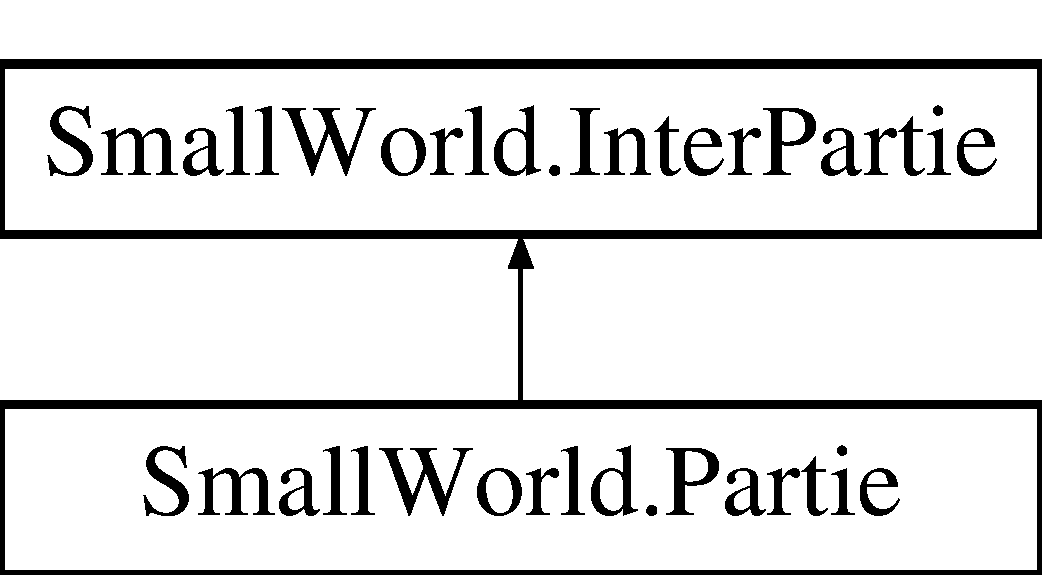
\includegraphics[height=2.000000cm]{class_small_world_1_1_partie}
\end{center}
\end{figure}
\subsection*{Public Member Functions}
\begin{DoxyCompactItemize}
\item 
\hypertarget{class_small_world_1_1_partie_a6123fa8d79551c91a92c7832649225b9}{void {\bfseries nouveau\-Tour} ()}\label{class_small_world_1_1_partie_a6123fa8d79551c91a92c7832649225b9}

\item 
\hypertarget{class_small_world_1_1_partie_aa76d3d1509ecdcb35fed3621455bab9f}{void {\bfseries selectionner\-Unite} ()}\label{class_small_world_1_1_partie_aa76d3d1509ecdcb35fed3621455bab9f}

\item 
\hypertarget{class_small_world_1_1_partie_abc458c09d880b2b16502bfe695439195}{void {\bfseries demander\-Deplacement} ()}\label{class_small_world_1_1_partie_abc458c09d880b2b16502bfe695439195}

\item 
\hypertarget{class_small_world_1_1_partie_a7ddc97d7833d234e06f18f0a97c6c15e}{void {\bfseries valider\-Tour} ()}\label{class_small_world_1_1_partie_a7ddc97d7833d234e06f18f0a97c6c15e}

\end{DoxyCompactItemize}
\subsection*{Properties}
\begin{DoxyCompactItemize}
\item 
\hypertarget{class_small_world_1_1_partie_a204fb33757e7ab7d0427a3c37f938062}{\hyperlink{class_small_world_1_1_joueur}{Joueur} {\bfseries Joueur}\hspace{0.3cm}{\ttfamily  \mbox{[}get, set\mbox{]}}}\label{class_small_world_1_1_partie_a204fb33757e7ab7d0427a3c37f938062}

\item 
\hypertarget{class_small_world_1_1_partie_a62ae701f7e4fa523001a6326c0033e6b}{\hyperlink{class_small_world_1_1_carte}{Carte} {\bfseries Carte}\hspace{0.3cm}{\ttfamily  \mbox{[}get, set\mbox{]}}}\label{class_small_world_1_1_partie_a62ae701f7e4fa523001a6326c0033e6b}

\item 
\hypertarget{class_small_world_1_1_partie_a76f9f56c84f30004462e65de85cbd1e3}{int {\bfseries nb\-Tour\-Restant}\hspace{0.3cm}{\ttfamily  \mbox{[}get, set\mbox{]}}}\label{class_small_world_1_1_partie_a76f9f56c84f30004462e65de85cbd1e3}

\end{DoxyCompactItemize}


The documentation for this class was generated from the following file\-:\begin{DoxyCompactItemize}
\item 
C\-:/\-Users/damienc/\-Documents/\-Git\-Hub/\-Small\-World/\-Visual\-Studio/\-Projet\-P\-O\-O/Partie.\-cs\end{DoxyCompactItemize}

\hypertarget{class_small_world_1_1_peuple}{\section{Small\-World.\-Peuple Class Reference}
\label{class_small_world_1_1_peuple}\index{Small\-World.\-Peuple@{Small\-World.\-Peuple}}
}
Inheritance diagram for Small\-World.\-Peuple\-:\begin{figure}[H]
\begin{center}
\leavevmode
\includegraphics[height=3.000000cm]{class_small_world_1_1_peuple}
\end{center}
\end{figure}
\subsection*{Public Member Functions}
\begin{DoxyCompactItemize}
\item 
\hypertarget{class_small_world_1_1_peuple_ae780348f6362ec2b371f58f0a2f696a1}{\hyperlink{interface_small_world_1_1_inter_unite}{Inter\-Unite} {\bfseries creer\-Unite} ()}\label{class_small_world_1_1_peuple_ae780348f6362ec2b371f58f0a2f696a1}

\end{DoxyCompactItemize}


The documentation for this class was generated from the following file\-:\begin{DoxyCompactItemize}
\item 
C\-:/\-Users/damienc/\-Documents/\-Git\-Hub/\-Small\-World/\-Visual\-Studio/\-Projet\-P\-O\-O/Peuple.\-cs\end{DoxyCompactItemize}

\hypertarget{class_small_world_1_1_peuple_gaulois}{\section{Small\-World.\-Peuple\-Gaulois Class Reference}
\label{class_small_world_1_1_peuple_gaulois}\index{Small\-World.\-Peuple\-Gaulois@{Small\-World.\-Peuple\-Gaulois}}
}
Inheritance diagram for Small\-World.\-Peuple\-Gaulois\-:\begin{figure}[H]
\begin{center}
\leavevmode
\includegraphics[height=3.000000cm]{class_small_world_1_1_peuple_gaulois}
\end{center}
\end{figure}
\subsection*{Public Member Functions}
\begin{DoxyCompactItemize}
\item 
\hypertarget{class_small_world_1_1_peuple_gaulois_a7c83ef827cd0a3202425487f8911776e}{\hyperlink{interface_small_world_1_1_inter_unite}{Inter\-Unite} {\bfseries creer\-Unite} ()}\label{class_small_world_1_1_peuple_gaulois_a7c83ef827cd0a3202425487f8911776e}

\end{DoxyCompactItemize}


The documentation for this class was generated from the following file\-:\begin{DoxyCompactItemize}
\item 
C\-:/\-Users/damienc/\-Documents/\-Git\-Hub/\-Small\-World/\-Visual\-Studio/\-Projet\-P\-O\-O/Peuple\-Gaulois.\-cs\end{DoxyCompactItemize}

\hypertarget{class_small_world_1_1_peuple_nain}{\section{Small\-World.\-Peuple\-Nain Class Reference}
\label{class_small_world_1_1_peuple_nain}\index{Small\-World.\-Peuple\-Nain@{Small\-World.\-Peuple\-Nain}}
}
Inheritance diagram for Small\-World.\-Peuple\-Nain\-:\begin{figure}[H]
\begin{center}
\leavevmode
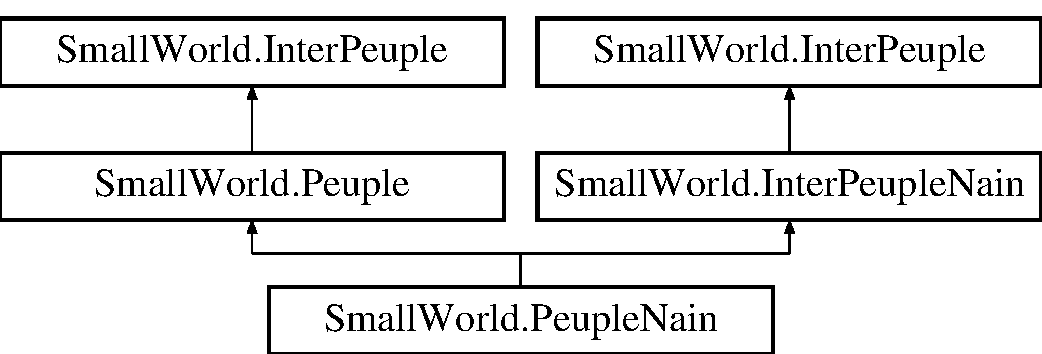
\includegraphics[height=3.000000cm]{class_small_world_1_1_peuple_nain}
\end{center}
\end{figure}
\subsection*{Public Member Functions}
\begin{DoxyCompactItemize}
\item 
\hypertarget{class_small_world_1_1_peuple_nain_ad200f4e7930232ab7ab89317795b8ee2}{new \hyperlink{interface_small_world_1_1_inter_unite}{Inter\-Unite} {\bfseries creer\-Unite} ()}\label{class_small_world_1_1_peuple_nain_ad200f4e7930232ab7ab89317795b8ee2}

\end{DoxyCompactItemize}


The documentation for this class was generated from the following file\-:\begin{DoxyCompactItemize}
\item 
C\-:/\-Users/damienc/\-Documents/\-Git\-Hub/\-Small\-World/\-Visual\-Studio/\-Projet\-P\-O\-O/Peuple\-Nain.\-cs\end{DoxyCompactItemize}

\hypertarget{class_small_world_1_1_peuple_viking}{\section{Small\-World.\-Peuple\-Viking Class Reference}
\label{class_small_world_1_1_peuple_viking}\index{Small\-World.\-Peuple\-Viking@{Small\-World.\-Peuple\-Viking}}
}


classe pour le peuple viking  


Inheritance diagram for Small\-World.\-Peuple\-Viking\-:\begin{figure}[H]
\begin{center}
\leavevmode
\includegraphics[height=3.000000cm]{class_small_world_1_1_peuple_viking}
\end{center}
\end{figure}
\subsection*{Public Member Functions}
\begin{DoxyCompactItemize}
\item 
\hyperlink{class_small_world_1_1_peuple_viking_aed3d04f06df7dadd594ede3f986d9ab1}{Peuple\-Viking} ()
\begin{DoxyCompactList}\small\item\em Constructeur d'un peuple viking. \end{DoxyCompactList}\item 
override \hyperlink{class_small_world_1_1_unite}{Unite} \hyperlink{class_small_world_1_1_peuple_viking_a28216d67245dc1c8db45b4c9d763923f}{creer\-Unite} ()
\begin{DoxyCompactList}\small\item\em création d'une unité viking \end{DoxyCompactList}\end{DoxyCompactItemize}


\subsection{Detailed Description}
classe pour le peuple viking 

\subsection{Constructor \& Destructor Documentation}
\hypertarget{class_small_world_1_1_peuple_viking_aed3d04f06df7dadd594ede3f986d9ab1}{\index{Small\-World\-::\-Peuple\-Viking@{Small\-World\-::\-Peuple\-Viking}!Peuple\-Viking@{Peuple\-Viking}}
\index{Peuple\-Viking@{Peuple\-Viking}!SmallWorld::PeupleViking@{Small\-World\-::\-Peuple\-Viking}}
\subsubsection[{Peuple\-Viking}]{\setlength{\rightskip}{0pt plus 5cm}Small\-World.\-Peuple\-Viking.\-Peuple\-Viking (
\begin{DoxyParamCaption}
{}
\end{DoxyParamCaption}
)}}\label{class_small_world_1_1_peuple_viking_aed3d04f06df7dadd594ede3f986d9ab1}


Constructeur d'un peuple viking. 

\begin{DoxyReturn}{Returns}
\hyperlink{class_small_world_1_1_peuple_viking}{Peuple\-Viking} un peuple viking 
\end{DoxyReturn}


\subsection{Member Function Documentation}
\hypertarget{class_small_world_1_1_peuple_viking_a28216d67245dc1c8db45b4c9d763923f}{\index{Small\-World\-::\-Peuple\-Viking@{Small\-World\-::\-Peuple\-Viking}!creer\-Unite@{creer\-Unite}}
\index{creer\-Unite@{creer\-Unite}!SmallWorld::PeupleViking@{Small\-World\-::\-Peuple\-Viking}}
\subsubsection[{creer\-Unite}]{\setlength{\rightskip}{0pt plus 5cm}Small\-World.\-Peuple\-Viking.\-creer\-Unite (
\begin{DoxyParamCaption}
{}
\end{DoxyParamCaption}
)\hspace{0.3cm}{\ttfamily [virtual]}}}\label{class_small_world_1_1_peuple_viking_a28216d67245dc1c8db45b4c9d763923f}


création d'une unité viking 

\begin{DoxyReturn}{Returns}
\hyperlink{class_small_world_1_1_unite}{Unite} une nouvelle unité 
\end{DoxyReturn}


Implements \hyperlink{class_small_world_1_1_peuple_a9d7edd46744bf12c7592b93342835a9b}{Small\-World.\-Peuple}.



The documentation for this class was generated from the following file\-:\begin{DoxyCompactItemize}
\item 
C\-:/\-Users/damienc/\-Documents/\-Git\-Hub/\-Small\-World/\-Visual\-Studio/\-Projet\-P\-O\-O/\hyperlink{_peuple_8cs}{Peuple.\-cs}\end{DoxyCompactItemize}

\hypertarget{class_small_world_1_1_plaine}{\section{Small\-World.\-Plaine Class Reference}
\label{class_small_world_1_1_plaine}\index{Small\-World.\-Plaine@{Small\-World.\-Plaine}}
}


class pour \hyperlink{class_small_world_1_1_case}{Case} de type plaine  


Inheritance diagram for Small\-World.\-Plaine\-:\begin{figure}[H]
\begin{center}
\leavevmode
\includegraphics[height=3.000000cm]{class_small_world_1_1_plaine}
\end{center}
\end{figure}


\subsection{Detailed Description}
class pour \hyperlink{class_small_world_1_1_case}{Case} de type plaine 

The documentation for this class was generated from the following file\-:\begin{DoxyCompactItemize}
\item 
C\-:/\-Users/damienc/\-Documents/\-Git\-Hub/\-Small\-World/\-Visual\-Studio/\-Projet\-P\-O\-O/\hyperlink{_case_8cs}{Case.\-cs}\end{DoxyCompactItemize}

\hypertarget{interface_small_world_1_1_sauvegarde}{\section{Small\-World.\-Sauvegarde Interface Reference}
\label{interface_small_world_1_1_sauvegarde}\index{Small\-World.\-Sauvegarde@{Small\-World.\-Sauvegarde}}
}
\subsection*{Public Member Functions}
\begin{DoxyCompactItemize}
\item 
\hypertarget{interface_small_world_1_1_sauvegarde_ac7bb1123afba8099288cab74e6a481cc}{void {\bfseries charge} ()}\label{interface_small_world_1_1_sauvegarde_ac7bb1123afba8099288cab74e6a481cc}

\item 
\hypertarget{interface_small_world_1_1_sauvegarde_a18e071e5ec26c588ca4d93f0e9f6acfb}{void {\bfseries enregistrer} ()}\label{interface_small_world_1_1_sauvegarde_a18e071e5ec26c588ca4d93f0e9f6acfb}

\end{DoxyCompactItemize}


The documentation for this interface was generated from the following file\-:\begin{DoxyCompactItemize}
\item 
C\-:/\-Users/damienc/\-Documents/\-Git\-Hub/\-Small\-World/\-Visual\-Studio/\-Projet\-P\-O\-O/Sauvegarder.\-cs\end{DoxyCompactItemize}

\hypertarget{class_small_world_1_1_strategie_carte}{\section{Small\-World.\-Strategie\-Carte Class Reference}
\label{class_small_world_1_1_strategie_carte}\index{Small\-World.\-Strategie\-Carte@{Small\-World.\-Strategie\-Carte}}
}
Inheritance diagram for Small\-World.\-Strategie\-Carte\-:\begin{figure}[H]
\begin{center}
\leavevmode
\includegraphics[height=2.901554cm]{class_small_world_1_1_strategie_carte}
\end{center}
\end{figure}
\subsection*{Public Member Functions}
\begin{DoxyCompactItemize}
\item 
void \hyperlink{class_small_world_1_1_strategie_carte_a451fff74bf423f6e225fd4816a7d1868}{construire} ()
\end{DoxyCompactItemize}


\subsection{Member Function Documentation}
\hypertarget{class_small_world_1_1_strategie_carte_a451fff74bf423f6e225fd4816a7d1868}{\index{Small\-World\-::\-Strategie\-Carte@{Small\-World\-::\-Strategie\-Carte}!construire@{construire}}
\index{construire@{construire}!SmallWorld::StrategieCarte@{Small\-World\-::\-Strategie\-Carte}}
\subsubsection[{construire}]{\setlength{\rightskip}{0pt plus 5cm}void Small\-World.\-Strategie\-Carte.\-construire (
\begin{DoxyParamCaption}
{}
\end{DoxyParamCaption}
)}}\label{class_small_world_1_1_strategie_carte_a451fff74bf423f6e225fd4816a7d1868}


Implements \hyperlink{interface_small_world_1_1_inter_strategie_carte_aa3f0d1267ad71756dc3b134d13733085}{Small\-World.\-Inter\-Strategie\-Carte}.



The documentation for this class was generated from the following file\-:\begin{DoxyCompactItemize}
\item 
C\-:/\-Users/damienc/\-Documents/\-Git\-Hub/\-Small\-World/\-Visual\-Studio/\-Projet\-P\-O\-O/Strategie\-Carte.\-cs\end{DoxyCompactItemize}

\hypertarget{class_small_world_1_1_strategie_demo}{\section{Small\-World.\-Strategie\-Demo Class Reference}
\label{class_small_world_1_1_strategie_demo}\index{Small\-World.\-Strategie\-Demo@{Small\-World.\-Strategie\-Demo}}
}
Inheritance diagram for Small\-World.\-Strategie\-Demo\-:\begin{figure}[H]
\begin{center}
\leavevmode
\includegraphics[height=3.000000cm]{class_small_world_1_1_strategie_demo}
\end{center}
\end{figure}
\subsection*{Public Member Functions}
\begin{DoxyCompactItemize}
\item 
void \hyperlink{class_small_world_1_1_strategie_demo_a6a9bbb801d3f894d735dc21d9029c2ee}{construire} ()
\end{DoxyCompactItemize}


\subsection{Member Function Documentation}
\hypertarget{class_small_world_1_1_strategie_demo_a6a9bbb801d3f894d735dc21d9029c2ee}{\index{Small\-World\-::\-Strategie\-Demo@{Small\-World\-::\-Strategie\-Demo}!construire@{construire}}
\index{construire@{construire}!SmallWorld::StrategieDemo@{Small\-World\-::\-Strategie\-Demo}}
\subsubsection[{construire}]{\setlength{\rightskip}{0pt plus 5cm}void Small\-World.\-Strategie\-Demo.\-construire (
\begin{DoxyParamCaption}
{}
\end{DoxyParamCaption}
)}}\label{class_small_world_1_1_strategie_demo_a6a9bbb801d3f894d735dc21d9029c2ee}


Implements \hyperlink{interface_small_world_1_1_inter_strategie_demo_a58c028866f521ee3e50ea0d7e94268e7}{Small\-World.\-Inter\-Strategie\-Demo}.



The documentation for this class was generated from the following file\-:\begin{DoxyCompactItemize}
\item 
C\-:/\-Users/damienc/\-Documents/\-Git\-Hub/\-Small\-World/\-Visual\-Studio/\-Projet\-P\-O\-O/Strategie\-Demo.\-cs\end{DoxyCompactItemize}

\hypertarget{class_small_world_1_1_strategie_normale}{\section{Small\-World.\-Strategie\-Normale Class Reference}
\label{class_small_world_1_1_strategie_normale}\index{Small\-World.\-Strategie\-Normale@{Small\-World.\-Strategie\-Normale}}
}
Inheritance diagram for Small\-World.\-Strategie\-Normale\-:\begin{figure}[H]
\begin{center}
\leavevmode
\includegraphics[height=3.000000cm]{class_small_world_1_1_strategie_normale}
\end{center}
\end{figure}
\subsection*{Public Member Functions}
\begin{DoxyCompactItemize}
\item 
void \hyperlink{class_small_world_1_1_strategie_normale_a7f3732b81d0b4b1e11dae277d6db219c}{construire} ()
\end{DoxyCompactItemize}


\subsection{Member Function Documentation}
\hypertarget{class_small_world_1_1_strategie_normale_a7f3732b81d0b4b1e11dae277d6db219c}{\index{Small\-World\-::\-Strategie\-Normale@{Small\-World\-::\-Strategie\-Normale}!construire@{construire}}
\index{construire@{construire}!SmallWorld::StrategieNormale@{Small\-World\-::\-Strategie\-Normale}}
\subsubsection[{construire}]{\setlength{\rightskip}{0pt plus 5cm}void Small\-World.\-Strategie\-Normale.\-construire (
\begin{DoxyParamCaption}
{}
\end{DoxyParamCaption}
)}}\label{class_small_world_1_1_strategie_normale_a7f3732b81d0b4b1e11dae277d6db219c}


Implements \hyperlink{interface_small_world_1_1_inter_strategie_normale_a6488d973a40d587a3357b6e690104258}{Small\-World.\-Inter\-Strategie\-Normale}.



The documentation for this class was generated from the following file\-:\begin{DoxyCompactItemize}
\item 
C\-:/\-Users/damienc/\-Documents/\-Git\-Hub/\-Small\-World/\-Visual\-Studio/\-Projet\-P\-O\-O/Strategie\-Normale.\-cs\end{DoxyCompactItemize}

\hypertarget{class_small_world_1_1_strategie_petite}{\section{Small\-World.\-Strategie\-Petite Class Reference}
\label{class_small_world_1_1_strategie_petite}\index{Small\-World.\-Strategie\-Petite@{Small\-World.\-Strategie\-Petite}}
}
Inheritance diagram for Small\-World.\-Strategie\-Petite\-:\begin{figure}[H]
\begin{center}
\leavevmode
\includegraphics[height=3.000000cm]{class_small_world_1_1_strategie_petite}
\end{center}
\end{figure}
\subsection*{Public Member Functions}
\begin{DoxyCompactItemize}
\item 
override void \hyperlink{class_small_world_1_1_strategie_petite_a19e5824d046b8dc0e982465195458192}{construire} ()
\end{DoxyCompactItemize}
\subsection*{Additional Inherited Members}


\subsection{Member Function Documentation}
\hypertarget{class_small_world_1_1_strategie_petite_a19e5824d046b8dc0e982465195458192}{\index{Small\-World\-::\-Strategie\-Petite@{Small\-World\-::\-Strategie\-Petite}!construire@{construire}}
\index{construire@{construire}!SmallWorld::StrategiePetite@{Small\-World\-::\-Strategie\-Petite}}
\subsubsection[{construire}]{\setlength{\rightskip}{0pt plus 5cm}override void Small\-World.\-Strategie\-Petite.\-construire (
\begin{DoxyParamCaption}
{}
\end{DoxyParamCaption}
)\hspace{0.3cm}{\ttfamily [virtual]}}}\label{class_small_world_1_1_strategie_petite_a19e5824d046b8dc0e982465195458192}


Implements \hyperlink{class_small_world_1_1_strategie_carte_a705ec27550d4dd65ec9295a851580c63}{Small\-World.\-Strategie\-Carte}.



The documentation for this class was generated from the following file\-:\begin{DoxyCompactItemize}
\item 
C\-:/\-Users/damienc/\-Documents/\-Git\-Hub/\-Small\-World/\-Visual\-Studio/\-Projet\-P\-O\-O/Strategie.\-cs\end{DoxyCompactItemize}

\hypertarget{class_small_world_1_1_unite}{\section{Small\-World.\-Unite Class Reference}
\label{class_small_world_1_1_unite}\index{Small\-World.\-Unite@{Small\-World.\-Unite}}
}
Inheritance diagram for Small\-World.\-Unite\-:\begin{figure}[H]
\begin{center}
\leavevmode
\includegraphics[height=3.000000cm]{class_small_world_1_1_unite}
\end{center}
\end{figure}
\subsection*{Public Member Functions}
\begin{DoxyCompactItemize}
\item 
\hypertarget{class_small_world_1_1_unite_a5e792891c8194bd5344cf1d3a897226a}{void {\bfseries attaquer} ()}\label{class_small_world_1_1_unite_a5e792891c8194bd5344cf1d3a897226a}

\item 
\hypertarget{class_small_world_1_1_unite_a51ba4ffd6b0029b1cc7be453f47730c5}{void {\bfseries deplacer} ()}\label{class_small_world_1_1_unite_a51ba4ffd6b0029b1cc7be453f47730c5}

\end{DoxyCompactItemize}


The documentation for this class was generated from the following file\-:\begin{DoxyCompactItemize}
\item 
C\-:/\-Users/damienc/\-Documents/\-Git\-Hub/\-Small\-World/\-Visual\-Studio/\-Projet\-P\-O\-O/Unite.\-cs\end{DoxyCompactItemize}

\hypertarget{class_small_world_1_1_unite_gauloise}{\section{Small\-World.\-Unite\-Gauloise Class Reference}
\label{class_small_world_1_1_unite_gauloise}\index{Small\-World.\-Unite\-Gauloise@{Small\-World.\-Unite\-Gauloise}}
}
Inheritance diagram for Small\-World.\-Unite\-Gauloise\-:\begin{figure}[H]
\begin{center}
\leavevmode
\includegraphics[height=3.000000cm]{class_small_world_1_1_unite_gauloise}
\end{center}
\end{figure}
\subsection*{Public Member Functions}
\begin{DoxyCompactItemize}
\item 
\hypertarget{class_small_world_1_1_unite_gauloise_a720db2403789106f4439a0601bbba9c5}{void {\bfseries attaquer} ()}\label{class_small_world_1_1_unite_gauloise_a720db2403789106f4439a0601bbba9c5}

\item 
\hypertarget{class_small_world_1_1_unite_gauloise_a1b925bc9484a883159a749c6ce8ceac4}{void {\bfseries deplacer} ()}\label{class_small_world_1_1_unite_gauloise_a1b925bc9484a883159a749c6ce8ceac4}

\end{DoxyCompactItemize}


The documentation for this class was generated from the following file\-:\begin{DoxyCompactItemize}
\item 
C\-:/\-Users/damienc/\-Documents/\-Git\-Hub/\-Small\-World/\-Visual\-Studio/\-Projet\-P\-O\-O/Unite\-Gauloise.\-cs\end{DoxyCompactItemize}

\hypertarget{class_small_world_1_1_unite_naine}{\section{Small\-World.\-Unite\-Naine Class Reference}
\label{class_small_world_1_1_unite_naine}\index{Small\-World.\-Unite\-Naine@{Small\-World.\-Unite\-Naine}}
}


Classe pour les unités naines.  


Inheritance diagram for Small\-World.\-Unite\-Naine\-:\begin{figure}[H]
\begin{center}
\leavevmode
\includegraphics[height=3.000000cm]{class_small_world_1_1_unite_naine}
\end{center}
\end{figure}
\subsection*{Public Member Functions}
\begin{DoxyCompactItemize}
\item 
\hyperlink{class_small_world_1_1_unite_naine_ae032047791cee62b77c1b7aed2e6f3da}{Unite\-Naine} ()
\begin{DoxyCompactList}\small\item\em Constructeur d'une unité naine. \end{DoxyCompactList}\item 
\hypertarget{class_small_world_1_1_unite_naine_aceabdf1ae46c14b18a9acfebe821a07b}{override void \hyperlink{class_small_world_1_1_unite_naine_aceabdf1ae46c14b18a9acfebe821a07b}{calcul\-Point\-Victoire} ()}\label{class_small_world_1_1_unite_naine_aceabdf1ae46c14b18a9acfebe821a07b}

\begin{DoxyCompactList}\small\item\em Met à jour les points de victoire apportés par l'unité \end{DoxyCompactList}\item 
override void \hyperlink{class_small_world_1_1_unite_naine_a487e42750e74fbf551d1e55b48101c72}{calculer\-Deplacement} ()
\begin{DoxyCompactList}\small\item\em met à jour les déplacements possibles \end{DoxyCompactList}\end{DoxyCompactItemize}
\subsection*{Additional Inherited Members}


\subsection{Detailed Description}
Classe pour les unités naines. 

\subsection{Constructor \& Destructor Documentation}
\hypertarget{class_small_world_1_1_unite_naine_ae032047791cee62b77c1b7aed2e6f3da}{\index{Small\-World\-::\-Unite\-Naine@{Small\-World\-::\-Unite\-Naine}!Unite\-Naine@{Unite\-Naine}}
\index{Unite\-Naine@{Unite\-Naine}!SmallWorld::UniteNaine@{Small\-World\-::\-Unite\-Naine}}
\subsubsection[{Unite\-Naine}]{\setlength{\rightskip}{0pt plus 5cm}Small\-World.\-Unite\-Naine.\-Unite\-Naine (
\begin{DoxyParamCaption}
{}
\end{DoxyParamCaption}
)}}\label{class_small_world_1_1_unite_naine_ae032047791cee62b77c1b7aed2e6f3da}


Constructeur d'une unité naine. 

\begin{DoxyReturn}{Returns}
une unité naine 
\end{DoxyReturn}


\subsection{Member Function Documentation}
\hypertarget{class_small_world_1_1_unite_naine_a487e42750e74fbf551d1e55b48101c72}{\index{Small\-World\-::\-Unite\-Naine@{Small\-World\-::\-Unite\-Naine}!calculer\-Deplacement@{calculer\-Deplacement}}
\index{calculer\-Deplacement@{calculer\-Deplacement}!SmallWorld::UniteNaine@{Small\-World\-::\-Unite\-Naine}}
\subsubsection[{calculer\-Deplacement}]{\setlength{\rightskip}{0pt plus 5cm}Small\-World.\-Unite\-Naine.\-calculer\-Deplacement (
\begin{DoxyParamCaption}
{}
\end{DoxyParamCaption}
)\hspace{0.3cm}{\ttfamily [virtual]}}}\label{class_small_world_1_1_unite_naine_a487e42750e74fbf551d1e55b48101c72}


met à jour les déplacements possibles 

\begin{DoxyReturn}{Returns}
void 
\end{DoxyReturn}


Implements \hyperlink{class_small_world_1_1_unite_a88ea1d2d5962c08ffc15422a2f2c7bbf}{Small\-World.\-Unite}.



The documentation for this class was generated from the following file\-:\begin{DoxyCompactItemize}
\item 
C\-:/\-Users/damienc/\-Documents/\-Git\-Hub/\-Small\-World/\-Visual\-Studio/\-Projet\-P\-O\-O/\hyperlink{_unite_8cs}{Unite.\-cs}\end{DoxyCompactItemize}

\hypertarget{class_small_world_1_1_unite_viking}{\section{Small\-World.\-Unite\-Viking Class Reference}
\label{class_small_world_1_1_unite_viking}\index{Small\-World.\-Unite\-Viking@{Small\-World.\-Unite\-Viking}}
}
Inheritance diagram for Small\-World.\-Unite\-Viking\-:\begin{figure}[H]
\begin{center}
\leavevmode
\includegraphics[height=3.000000cm]{class_small_world_1_1_unite_viking}
\end{center}
\end{figure}
\subsection*{Additional Inherited Members}


The documentation for this class was generated from the following file\-:\begin{DoxyCompactItemize}
\item 
C\-:/\-Users/damienc/\-Documents/\-Git\-Hub/\-Small\-World/\-Visual\-Studio/\-Projet\-P\-O\-O/Unite\-Viking.\-cs\end{DoxyCompactItemize}

\hypertarget{interface_small_world_1_1_viking}{\section{Small\-World.\-Viking Interface Reference}
\label{interface_small_world_1_1_viking}\index{Small\-World.\-Viking@{Small\-World.\-Viking}}
}


The documentation for this interface was generated from the following file\-:\begin{DoxyCompactItemize}
\item 
C\-:/\-Users/damienc/\-Documents/\-Git\-Hub/\-Small\-World/\-Visual\-Studio/\-Projet\-P\-O\-O/Viking.\-cs\end{DoxyCompactItemize}

\chapter{File Documentation}
\hypertarget{_carte_8cs}{\section{C\-:/\-Users/damienc/\-Documents/\-Git\-Hub/\-Small\-World/\-Visual\-Studio/\-Projet\-P\-O\-O/\-Carte.cs File Reference}
\label{_carte_8cs}\index{C\-:/\-Users/damienc/\-Documents/\-Git\-Hub/\-Small\-World/\-Visual\-Studio/\-Projet\-P\-O\-O/\-Carte.\-cs@{C\-:/\-Users/damienc/\-Documents/\-Git\-Hub/\-Small\-World/\-Visual\-Studio/\-Projet\-P\-O\-O/\-Carte.\-cs}}
}


Interface et classe de la Carte.  


\subsection*{Classes}
\begin{DoxyCompactItemize}
\item 
interface \hyperlink{interface_small_world_1_1_inter_carte}{Small\-World.\-Inter\-Carte}
\begin{DoxyCompactList}\small\item\em Interface pour \hyperlink{class_small_world_1_1_carte}{Carte}. \end{DoxyCompactList}\item 
class \hyperlink{class_small_world_1_1_carte}{Small\-World.\-Carte}
\begin{DoxyCompactList}\small\item\em Classe \hyperlink{class_small_world_1_1_carte}{Carte} Représente la carte du monde. \end{DoxyCompactList}\end{DoxyCompactItemize}
\subsection*{Namespaces}
\begin{DoxyCompactItemize}
\item 
package \hyperlink{namespace_small_world}{Small\-World}
\end{DoxyCompactItemize}


\subsection{Detailed Description}
Interface et classe de la Carte. Une Carte représente le plateau de jeu et se compose d'un ensemble de Case, de type différent

\begin{DoxyAuthor}{Author}
\href{mailto:damien.cremilleux@insa-rennes.fr}{\tt Damien Crémilleux} 

\href{mailto:lauriane.holy@insa-rennes.fr}{\tt Lauriane Holy}
\end{DoxyAuthor}
\begin{DoxyDate}{Date}
15/12/2013 
\end{DoxyDate}
\begin{DoxyVersion}{Version}
0.\-1 
\end{DoxyVersion}

\hypertarget{_createur_partie_8cs}{\section{C\-:/\-Users/damienc/\-Documents/\-Git\-Hub/\-Small\-World/\-Visual\-Studio/\-Projet\-P\-O\-O/\-Createur\-Partie.cs File Reference}
\label{_createur_partie_8cs}\index{C\-:/\-Users/damienc/\-Documents/\-Git\-Hub/\-Small\-World/\-Visual\-Studio/\-Projet\-P\-O\-O/\-Createur\-Partie.\-cs@{C\-:/\-Users/damienc/\-Documents/\-Git\-Hub/\-Small\-World/\-Visual\-Studio/\-Projet\-P\-O\-O/\-Createur\-Partie.\-cs}}
}


Interface et classe du créateur de partie.  


\subsection*{Classes}
\begin{DoxyCompactItemize}
\item 
interface \hyperlink{interface_small_world_1_1_inter_createur_partie}{Small\-World.\-Inter\-Createur\-Partie}
\begin{DoxyCompactList}\small\item\em Interface du créateur de partie. \end{DoxyCompactList}\item 
class \hyperlink{class_small_world_1_1_createur_partie}{Small\-World.\-Createur\-Partie}
\begin{DoxyCompactList}\small\item\em Classe du créateur de partie. \end{DoxyCompactList}\end{DoxyCompactItemize}
\subsection*{Namespaces}
\begin{DoxyCompactItemize}
\item 
package \hyperlink{namespace_small_world}{Small\-World}
\end{DoxyCompactItemize}


\subsection{Detailed Description}
Interface et classe du créateur de partie. Directeur du patron de conception Monteur, contient le processus de création

\begin{DoxyAuthor}{Author}
\href{mailto:damien.cremilleux@insa-rennes.fr}{\tt Damien Crémilleux} 

\href{mailto:lauriane.holy@insa-rennes.fr}{\tt Lauriane Holy}
\end{DoxyAuthor}
\begin{DoxyDate}{Date}
15/01/2014 
\end{DoxyDate}
\begin{DoxyVersion}{Version}
0.\-1 
\end{DoxyVersion}

\hypertarget{_monteur_partie_8cs}{\section{C\-:/\-Users/damienc/\-Documents/\-Git\-Hub/\-Small\-World/\-Visual\-Studio/\-Projet\-P\-O\-O/\-Monteur\-Partie.cs File Reference}
\label{_monteur_partie_8cs}\index{C\-:/\-Users/damienc/\-Documents/\-Git\-Hub/\-Small\-World/\-Visual\-Studio/\-Projet\-P\-O\-O/\-Monteur\-Partie.\-cs@{C\-:/\-Users/damienc/\-Documents/\-Git\-Hub/\-Small\-World/\-Visual\-Studio/\-Projet\-P\-O\-O/\-Monteur\-Partie.\-cs}}
}


Interfaces et classes du monteur de partie.  


\subsection*{Classes}
\begin{DoxyCompactItemize}
\item 
interface \hyperlink{interface_small_world_1_1_inter_monteur_partie}{Small\-World.\-Inter\-Monteur\-Partie}
\begin{DoxyCompactList}\small\item\em Interface globale du monteur. \end{DoxyCompactList}\item 
interface \hyperlink{interface_small_world_1_1_inter_monteur_partie_demo}{Small\-World.\-Inter\-Monteur\-Partie\-Demo}
\begin{DoxyCompactList}\small\item\em Interface du monteur de partie démo. \end{DoxyCompactList}\item 
interface \hyperlink{interface_small_world_1_1_inter_monteur_partie_petite}{Small\-World.\-Inter\-Monteur\-Partie\-Petite}
\begin{DoxyCompactList}\small\item\em Interface du monteur de partie petite. \end{DoxyCompactList}\item 
interface \hyperlink{interface_small_world_1_1_inter_monteur_partie_normale}{Small\-World.\-Inter\-Monteur\-Partie\-Normale}
\begin{DoxyCompactList}\small\item\em Interface du monteur de partie normale. \end{DoxyCompactList}\item 
class \hyperlink{class_small_world_1_1_monteur_partie}{Small\-World.\-Monteur\-Partie}
\begin{DoxyCompactList}\small\item\em Classe abstraite implémentant Inter\-Monteur \hyperlink{interface_small_world_1_1_inter_partie}{Inter\-Partie}. \end{DoxyCompactList}\item 
class \hyperlink{class_small_world_1_1_monteur_partie_demo}{Small\-World.\-Monteur\-Partie\-Demo}
\begin{DoxyCompactList}\small\item\em classe pour un monteur d'une partie démo \end{DoxyCompactList}\item 
class \hyperlink{class_small_world_1_1_monteur_partie_petite}{Small\-World.\-Monteur\-Partie\-Petite}
\begin{DoxyCompactList}\small\item\em classe pour un monteur d'une partie petite \end{DoxyCompactList}\item 
class \hyperlink{class_small_world_1_1_monteur_partie_normale}{Small\-World.\-Monteur\-Partie\-Normale}
\begin{DoxyCompactList}\small\item\em classe pour un monteur d'une partie normale \end{DoxyCompactList}\end{DoxyCompactItemize}
\subsection*{Namespaces}
\begin{DoxyCompactItemize}
\item 
package \hyperlink{namespace_small_world}{Small\-World}
\end{DoxyCompactItemize}


\subsection{Detailed Description}
Interfaces et classes du monteur de partie. Monteur du patron de conception monteur, contient les interfaces et les différentes implémentations pour le processus de création d'une partie

\begin{DoxyAuthor}{Author}
\href{mailto:damien.cremilleux@insa-rennes.fr}{\tt Damien Crémilleux} 

\href{mailto:lauriane.holy@insa-rennes.fr}{\tt Lauriane Holy}
\end{DoxyAuthor}
\begin{DoxyDate}{Date}
15/01/2014 
\end{DoxyDate}
\begin{DoxyVersion}{Version}
0.\-1 
\end{DoxyVersion}

%--- End generated contents ---

% Index
\newpage
\phantomsection
\addcontentsline{toc}{part}{Index}
\printindex

\end{document}
